

\begin{filecontents*}{\jobname.bib}

@case{keyabc,
  partya = {ABC}, 
  partyb = {XYZ*},
  caseyear = {2016},
  reportyear={2020},
  reportvolume = {3},
  volyearneeded = {true},
  reportseries = {WLR},
  reportpage = {123},
  courtname = {XYZCA},
  casenumber = {456},
	}

@case{case2,
  partya = {DDA}, 
  partyb = {MNO*},
  caseyear = {2019},
%  reportvolume = {3},
%  volyearneeded = {true},
%  reportseries = {WLR},
%  reportpage = {123},
  courtname = {HACCA},
  casenumber = {14},
	}
@case{case3,
  partya = {Efg}, 
  partyb = {Hij*},
  caseyear = {2018},
%  reportvolume = {3},
%  volyearneeded = {true},
%  reportseries = {WLR},
%  reportpage = {123},
  courtname = {VFC},
  casenumber = {1},
	}
@case{case4,
  partya = {Klm}, 
  partyb = {Nop*},
  caseyear = {2015},
  reportyear={2016},
  reportvolume = {2},
  volyearneeded = {true},
  reportseries = {WLR},
  reportpage = {25},
  courtname = {MBC},
  casenumber = {21},
	}
@case{case5,
  partya = {No MNC A}, 
  partyb = {No MNC B*},
  reportyear={1757},
  reportvolume = {1},
%  volyearneeded = {true},
  reportseries = {Co},
  reportpage = {25},
	}
@book{book1,
	title={A Title*},
	author={B Auctoritas},
	year={1828},
	publisher={Holmes and Sons},
	}



@case{becher,
  partya = {City of Columbus}, 
  partyb = {Becher},
%  reportyear={},
  reportvolume = {180},
%  volyearneeded = {true},
  reportseries = {NE 2d},
  reportpage = {836},
  year = {1962},
  note = {Ohio, Zimmerman J},
	}


@case{cassie,
  partya = {Cassie}, 
  partyb = {Koumans},
  caseshortname = {Cassie},
  caseyear = {2007},
%	  reportyear={2016},
%	  reportvolume = {2},
%	  volyearneeded = {true},
%	  reportseries = {WLR},
%	  reportpage = {25},
  courtname = {NSWSC},
  casenumber = {481},
	}


@case{becker,
  partya = {City of Marion}, 
  partyb = {Becker},
  caseshortname = {Becker},
%  caseyear = {2007},
  reportyear={1973},
  reportvolume = {6},
%  volyearneeded = {},
  reportseries = {SASR},
  reportpage = {13},
%  courtname = {NSWSC},
%  casenumber = {481},
	}

%R v Morgan [1970] 3 All ER 1053
@case{rmorgan,
  partya = {R}, 
  partyb = {Morgan},
  caseshortname = {Morgan},
  reportyear={1970},
  reportvolume = {3},
  volyearneeded = {true},
  reportseries = {All ER},
  reportpage = {1053},
	}


@book{eco,
author={Umberto Eco},
title={Come si fa una tesi di laurea},
subtitle={Le materie umanistiche},
title+an = {How to write a Thesis for an Arts Degree},
publisher={Bompiani},
date={2004},
origdate={1977},
edition={15},
options={skipbib=true},
%isbn={9788845246310},
}

@book{anncrimnsw,
author={Roderick N Howie and Peter A Johnson},
title={Annotated Criminal Legislation New South Wales},
publisher={LexisNexis Butterworths},
date={2015},
edition={2014-2015},
}

@case{columbus,
  partya = {City of Columbus},
  partyashortname = {Columbus}, 
  partyb = {Becher},
  caseshortname = {Becher},
  icaseyear = {1962},
  jurisdiction = {Ohio},
  courtfullname = {Supreme Court of Ohio},
  note = {Ohio SC, 1962},
	}
@case{columbussr,
  reportvolume = {173},
  reportseries = {Ohio St},
  reportpage = {197},
  crossref = {columbus},
}

@case{columbusne,
  reportvolume = {180},
  reportseries = {NE 2d},
  reportseriesseries = {2d},
  reportpage = {836},
  crossref = {columbus},
}
%%%%%%%%%%%%%

@xdata{xcolumbus,
  partya = {xCity of Columbus},
  partyashortname = {Columbus}, 
  partyb = {Becher},
  year = {1962},
  jurisdiction = {Ohio},
  courtfullname = {Supreme Court of Ohio},
  note = {Ohio SC, 1962},
	}
	
@case{xcolumbussr,
  reportvolume = {173},
  reportseries = {Ohio St},
  reportpage = {197},
  xdata = {xcolumbus},
}

@case{xcolumbusne,
  reportvolume = {180},
  reportseries = {NE 2d},
  reportseriesseries = {2d},
  reportpage = {836},
  xdata = {xcolumbus},
}


%%%%%%%%%%%%%
@case{thomas,
  partya = {Thomas},
  partyb = {Newton*},
  icaseyear = {1827},
	}

@case{thomascar,
  reportyear = {1827},
  reportvolume = {2},
  reportseries = {Car \& P},
  reportpage = {606},
  crossref = {thomas},
}

@case{thomaser,
  reportvolume = {?},
  reportseries = {ER},
  reportpage = {276},
  crossref = {thomas},
}

@case{thomasermnc,
  caseyear = {1827},
  courtname = {EngRep},
  casenumber = {503},
  crossref = {thomas},
}


@case{gitlow,
  partya = {Gitlow},
  partyb = {New York},%People of New York
  partyashortname = {New York}, 
  caseshortname = {Gitlow},
  icaseyear = {1925},
  note = {1925},
	}


@case{gitlowus,
  reportvolume = {268},
  reportseries = {US},
  reportpage = {652},
  crossref = {gitlow},
}


@case{gitlowsc,
  reportvolume = {45},
  reportseries = {SCt},
  reportpage = {625},
  crossref = {gitlow},
}

@case{armstrong,
  partya = {Adam Armstrong's Case},
  icaseyear = {1823},
  caseshortname = {Armstrong},
	}

@case{armstrongmnc,
  caseyear = {1823},
  courtname = {EngR},
  casenumber = {1},
  crossref = {armstrong},
}


@case{armstronglewin,
  reportyear = {1823},
  reportvolume = {1},
  reportseries = {Lewin},
  reportpage = {245},
  crossref = {armstrong},
}

@case{armstronger,
  reportvolume = {168},
  reportseries = {ER},
  reportpage = {1028},
  crossref = {armstrong},
}


%Adam Armstrong's Case [1823] EngR 1; (1823) 1 Lewin 245; 168 E.R. 1028 (1 January 1823)


@case{alexander,
  partya = {Alexander},
  partyb = {Brown},
  icaseyear = {1823},
  caseshortname = {Alexander},
	}

@case{alexandermnc,
  caseyear = {1823},
  courtname = {EngR},
  casenumber = {5},
  crossref = {alexander},
}


@case{alexandercp,
  reportyear = {1823-1825},
  reportvolume = {1},
  reportseries = {C \& P},
  reportpage = {288},
  crossref = {alexander},
}

@case{alexanderer,
  reportvolume = {171},
  reportseries = {ER},
  reportpage = {1199},
  crossref = {alexander},
  note = {A},
}



%Alexander v Brown [1823] EngR 5; (1823-1825) 1 Car & P 288; 171 E.R. 1199 (A) (1 January 1823)

@book{bishop,
author = {Joel Prentiss Bishop},
title = {The First Book of the Law},
date = {1868},
publisher = {Little, Brown, and Company},
location = {Boston},
}


@case{velocity,
  partya = {shipname Velocity},
  icaseyear = {1869},
  shipname = {Velocity},
	}

@case{velocitymnc,
  caseyear = {1869},
  courtname = {EngR},
  casenumber = {53},
  crossref = {velocity},
}


@case{velocitynr,
  reportyear = {1869},
  reportvolume = {6},
  reportseries = {Moo PC NS},
  reportpage = {263},
  crossref = {velocity},
}

@case{velocityer,
  reportvolume = {16},
  reportseries = {ER},
  reportpage = {725},
  crossref = {velocity},
}



%The "Velocity" [1869] EngR 53; (1869) 6 Moo PC NS 263; 16 E.R. 725


@case{snail,
  partya = {Donoghue}, 
  partyb = {Stevenson},
  icaseyear = {1932},
  reportyear={1932},
%  volyearneeded = {true},
  reportseries = {AC},
  reportpage = {562},
  casenickname = {snail in the bottle},
  note = {HL},
	}

%Commonwealth v Tasmania ("Tasmanian Dam case") [1983] HCA 21; (1983) 158 CLR 1

@case{tasdam,
  partya = {Commonwealth}, 
  partyb = {Tasmania},
  icaseyear = {1983},
  casenickname = {Tasmanian Dam},
  }
@case{tasdammnc,
  caseyear = {1983},
  courtname = {HCA},
  casenumber = {2},
  crossref = {tasdam},
  }
@case{tasdamclr,
  reportyear={1983},
%  volyearneeded = {true},
  reportvolume = {158},
  reportseries = {CLR},
  reportpage = {1},
  crossref = {tasdam},
  	}
@case{frame,
  partya = {Frame}, 
  partyb = {Smith},
  icaseyear = {1987},
  }
@case{framescr,
  reportyear = {1987},
  volyearneeded = {true},
  reportvolume = {2},
  reportseries = {SCR},
  reportpage = {99},
  crossref = {frame},
  }
@case{framedlr,
  reportvolume = {42},
  reportseries = {DLR (4th)},
  reportpage = {81},
  crossref = {frame},
  	}








%Dow Jones and Company Inc v Gutnick [2002] HCA 56; 210 CLR 575; 194 ALR 433; 77 ALJR 255 (10 December 2002)

@case{gutnick,
  partya = {Dow Jones and Company Inc}, 
  partyb = {Gutnick},
  icaseyear = {2002},
  }
@case{gutnickmnc,
  caseyear = {2002},
  courtname = {HCA},
  casenumber = {56},
  crossref = {gutnick},
  }
@case{gutnickclr,
%  reportyear={1983},
%  volyearneeded = {true},
  reportvolume = {210},
  reportseries = {CLR},
  reportpage = {575},
  crossref = {gutnick},
  	}
@case{gutnickalr,
%  reportyear={1983},
%  volyearneeded = {true},
  reportvolume = {194},
  reportseries = {ALR},
  reportpage = {433},
  crossref = {gutnick},
  	}
@case{gutnickaljr,
%  reportyear={1983},
%  volyearneeded = {true},
  reportvolume = {77},
  reportseries = {ALJR},
  reportpage = {255},
  crossref = {gutnick},
  	}




%Kerr v Baranow, 2011 SCC 10, [2011] 1 SCR 269

@case{kerr,
  partya = {Kerr}, 
  partyb = {Baranow},
  icaseyear = {2011},
  }
@case{kerrmnc,
  caseyear = {2011},
  courtname = {SCC},
  casenumber = {10},
  crossref = {kerr},
  }
@case{kerrscr,
  reportyear={2011},
  volyearneeded = {true},
  reportvolume = {1},
  reportseries = {SCR},
  reportpage = {269},
  crossref = {kerr},
  	}



%McLean v Pilon (1978), 7 BCLR 99, 1978 CanLII 237 (SC).


@case{mclean,
  partya = {McLean}, 
  partyb = {Pilon},
  icaseyear = {1978},
  decisionyear = {1978},
  note = {SC},
  }
@case{mcleanlii,
  caseyear = {1978},
  courtname = {CanLII},
  casenumber = {237},
  crossref = {mclean},
  }
@case{mcleanbclr,
%  reportyear={2011},
%  volyearneeded = {true},
  reportvolume = {7},
  reportseries = {BCLR},
  reportpage = {99},
  crossref = {mclean},
  	}








%Smyth, Russell --- "What do Intermediate Appellate Courts Cite? A Quantitative Study of the Citation Practice of Australian State Supreme Courts" [1999] AdelLawRw 3; (1999) 21 Adelaide Law Review 51

@article{smythsc,
author = {Russell Smyth},
title = {What do Intermediate Appellate Courts Cite? A Quantitative Study of the Citation Practice of Australian State Supreme Courts},
mncyear = {1999},
mncname = {AdelLawRw},
mncnumber = {3},
date = {1999},
volume = {21},
journaltitle = {Adelaide Law Review},
pages = {51},
keywords = {lj},
}



%=================== law journal articles


@ljarticle{ljart3,
options={year-required=true,},
author={given=qqq, family=rrr},
title ={A Third Legal Article yr req},
journaltitle={MNOLR},
date={2016},
volume={1},
pages={458},
}

@book{b2035,title ={Chitty on Contracts},edition ={26},publisher ={Sweet and Maxwell},date ={1989},}
@book{b2036,title ={Clerk and Lindsell on Torts},edition ={16},publisher ={Sweet and Maxwell},date ={1989},}

@periodical{j76,journaltitle={Modern Law Review},volume={54},number={1},month={1},date={1991},}

%b2035,
@article{a104,
author={Ewan McKendrick},
related={b2035,b2036},
relatedtype={reviewof},
crossref={j76},
pages={162},
keywords={otl, lj},
}


%Lawrence Friedman, Robert Kagan, Bliss Cartwright and Stanton
%Wheeler, 'State Supreme Courts: A Century of Style and Citation' (1981) 33 Stanford Law
%Review 773 (covering 16 state supreme courts in the period 1870-1970).


@article{friedman,
author = {Lawrence Friedman and Robert Kagan and Bliss Cartwright and Stanton Wheeler},
title = {State Supreme Courts},
subtitle = {A Century of Style and Citation},
%mncyear = {1999},
%mncname = {AdelLawRw},
%mncnumber = {3},
date = {1981},
volume = {33},
journaltitle = {Stanford Law Review},
pages = {773},
%---
%reportyear = {1981},
%repotrvolume = {33},
%reportname = {Stanford Law Review},
%reportpage = {773},
note = {covering 16 state supreme courts in the period 1870-1970},
keywords = {lj},
}



@book{butt,
author = {Peter Butt},
title={Legal Usage},
subtitle={A Modern Style Guide},
date={2018},
publisher={LexisNexis Butterworths},
}


@statute{crimnsw,
statutetitle = {Crimes Act},
%statutelongtitle = {},
%statuteshorttitle = {},
%statutenickname = {},
%statutevolume = {},
statutejurisdiction = {NSW},
%statuteregnalyear = {},
%statutechapter = {},
%statuteyear = {},%for the volume
statutetitleyear = {1900},%for the title
}

%Criminal Code, RSC 1985, c C-46, s 515

@statute{crimcan,
statutetitle = {Criminal Code},
%statutelongtitle = {},
%statuteshorttitle = {},
%statutenickname = {},
%statutevolume = {},
%statutejurisdiction = {NSW},
%statuteregnalyear = {},
%statutechapter = {},
%statuteyear = {},%for the volume
statutetitleyear = {RSC 1985, c C-46},%for the title
}


@statute{canreg,
statutetitle = {Maple Products Regulations},
%statutelongtitle = {},
statuteshorttitle = {CRC},
%statutenickname = {},
%statutevolume = {},
%statutejurisdiction = {NSW},
%statuteregnalyear = {},
statutechapter = {289},
%statuteyear = {},%for the volume
%statutetitleyear = {RSC 1985},%for the title
}

@statute{testregs,
statutetitle = {Test Regs},
statutetitleyear = {2020},%for the title
keywords = {regulations},
statutejurisdiction = {NSW},
}




@statute{crimcodecan,
citeref = {canleg},
title = {Criminal Code},
svjy = {RSC 1985},
chapter = {C-46},
}


@statute{oescheats,
citeref = {canleg},
title = {Escheats Act},
svjy = {RSO 1980},
chapter = {142},
}

@statute{canleg,
citeref = {canleg},
title = {Copyright Act},
chapter = {C-42},
svjy = {RSC 1985},
%year = {xxx},
%regnum = {xxx},
}

@statute{canregcrc,
citeref = {crcreg},
title = {Maple Products Regulations},
chapter = {289},
%year = {xxx},
%regnum = {xxx},
}


@statute{canregsor,
citeref = {sorreg},
title = {Regulations Amending the Food and Drug Regulations},
%chapter = {xxx},
year = {98},
regnum = {580},
}

@statute{canregalta,
citeref = {altareg},
%title = {xxx},
%chapter = {xxx},
year = {2009},
regnum = {62},
}

@statute{canregbc,
citeref = {bcreg},
%title = {xxx},
%chapter = {xxx},
year = {2008},
regnum = {278},
}

@statute{canregman,
citeref = {manreg},
%title = {xxx},
%chapter = {xxx},
year = {87},
regnum = {351},
}
@statute{canregnb,
citeref = {nbreg},
%title = {xxx},
%chapter = {xxx},
year = {2006},
regnum = {23},
}
@statute{canregnfld,
citeref = {nfldreg},
%title = {xxx},
%chapter = {xxx},
year = {97},
regnum = {19},
}
@statute{canregnlr,
citeref = {nlrreg},
%title = {xxx},
%chapter = {xxx},
year = {09},
regnum = {4},
}
@statute{canregnwt,
citeref = {nwtreg},
%title = {xxx},
%chapter = {xxx},
year = {2008},
regnum = {26},
}
@statute{canregns,
citeref = {nsreg},
%title = {xxx},
%chapter = {xxx},
year = {2007},
regnum = {235},
}
@statute{canregnu,
citeref = {nureg},
%title = {xxx},
%chapter = {xxx},
year = {040},
regnum = {99},
}
@statute{canrego,
citeref = {oreg},
%title = {xxx},
%chapter = {xxx},
year = {08},
regnum = {361},
}
@statute{canregpei,
citeref = {peireg},
%title = {xxx},
%chapter = {xxx},
year = {2002},
regnum = {249},
}

@statute{canregoc,
citeref = {ocreg},
%title = {xxx},
%chapter = {xxx},
year = {97},
regnum = {764},
fulldate = {25 June 1997},
gazette = {1997.II.2737},
}

@statute{canregsask,
citeref = {saskreg},
%title = {xxx},
%chapter = {xxx},
year = {67},
regnum = {444},
}

@statute{canregyoic,
citeref = {yoicreg},
%title = {xxx},
%chapter = {xxx},
year = {1995},
regnum = {87},
}







\end{filecontents*}




\begin{filecontents*}{lawcite.dbx}
%hyperref support for splitindex
%\NewDocumentCommand\boldhyperpage{ m } {\textbf{\hyperpage{#1}}
%\NewDocumentCommand\boldhyperpage{ m } {\hyperpage{#1}}

\DeclareDatamodelFields[type=field, datatype=verbatim]{thumbnail}
\DeclareDatamodelEntryfields{thumbnail}

\newcommand*{\insertbibimage}[1]{\includegraphics[width=1cm, keepaspectratio]{#1}}

%
\newtoggle{printregulations}
\toggletrue{printregulations}

%
\newtoggle{printxregulations}
\toggletrue{printxregulations}


%\newbibmacro{lctor}{%
\newcommand\lctor{%
%\ifkeyword{regulations}{\iftoggle{printregulations}{regulations}{legislation}}{legislation}%
\iftoggle{printxregulations}{regulations}{legislation}%
%legislation%
}




\DeclareDatamodelEntrytypes{case,statute}
\DeclareDatamodelFields[type=field, datatype=literal]{
% case fields
  partya, 
  partyb,
  partysep,
  shipname,
  caseyear, %will be a date
  icaseyear, %for the index
  decisionyear, %for the casename, when no report year
  reportyear, %will be a date
  reportvolume,
  volyearneeded, %will be a boolean
  reportseries,
  reportpage,
  courtname,
  casenumber,
  note,
  caseshortname,
  casenickname,
% statute
statutetitle,
statutelongtitle,
statuteshorttitle,
statutenickname,
statutevolume,
statutejurisdiction,
statuteregnalyear,
statutechapter,
statuteyear,%for the volume
statutetitleyear,%for the title
%reg2
title,
chapter,
year,
citeref,
regnum,
fulldate,
gazette,
%leg
svjy,
}

\DeclareDatamodelEntryfields[case]{%
partya,partyb,partysep,caseyear,reportyear,reportvolume,%
volyearneeded,reportseries,reportpage,courtname,casenumber,note,shipname,%
icaseyear,caseshortname,casenickname,decisionyear}


\DeclareDatamodelEntryfields[statute]{%
statutetitle,%
statutelongtitle,%
statuteshorttitle,%
statutenickname,%
statutevolume,%
statutejurisdiction,%
statuteregnalyear,%
statutechapter,%
statuteyear,%for the volume
statutetitleyear,%for the title
%reg2
title,%
chapter,%
year,%
citeref,%
regnum,%
fulldate,%
gazette,%
%
svjy,%
}


\DeclareLanguageMapping{english}{english-lawcite}


\endinput
\end{filecontents*}

\begin{filecontents*}{lawcite.bbx}
\ProvidesFile{lawcite.bbx}[2020/04/11 v1.0 biblatex bibliography style]
\RequireBibliographyStyle{ext-authortitle-ibid}
%%%%%%%%% case
\newtoggle{partysepitalic}
\toggletrue{partysepitalic}
%
\newtoggle{partysepdotted}
\togglefalse{partysepdotted}
%
\newtoggle{partynamesitalic}
\toggletrue{partynamesitalic}
%
\newcounter{reftypemode}
\setcounter{reftypemode}{3}%default: 3 allbelow
%
\newtoggle{mncbrackets}
\toggletrue{mncbrackets}
%
\newtoggle{multicitecomma}
\togglefalse{multicitecomma}
%
\newtoggle{printlegtoc}\toggletrue{printlegtoc}
%
\newtoggle{refintoc}\toggletrue{refintoc}
%
%%%%%%%%% statute
\newtoggle{statjurisdiction}
\togglefalse{statjurisdiction}
%
\newtoggle{stattycomma}
\togglefalse{stattycomma}
%
\newtoggle{stattyitalic}
\togglefalse{stattyitalic}
%
\newtoggle{lcindexing}
\toggletrue{lcindexing}

% statute
\DeclareBibliographyOption[boolean]{set-lawcite-indexing}[true]{%
\ifstrequal{#1}{true}
{\toggletrue{lcindexing}}
{\togglefalse{lcindexing}}%
}
%

% statute
\DeclareBibliographyOption[boolean]{regulations-as-tor}[true]{%
\ifstrequal{#1}{true}
{\toggletrue{printregulations}\toggletrue{printxregulations}}
{\togglefalse{printregulations}\togglefalse{printxregulations}}%
}
%
\DeclareBibliographyOption[boolean]{show-statute-jurisdiction}[false]{%
\ifstrequal{#1}{true}
{\toggletrue{statjurisdiction}}
{\togglefalse{statjurisdiction}}%
}
%
\DeclareBibliographyOption[boolean]{statute-title-year-comma}[false]{%
\ifstrequal{#1}{true}
{\toggletrue{stattycomma}}
{\togglefalse{stattycomma}}%
}
%
\DeclareBibliographyOption[boolean]{statute-title-year-italic}[false]{%
\ifstrequal{#1}{true}
{\toggletrue{stattyitalic}}
{\togglefalse{stattyitalic}}%
}

%
\newtoggle{indemomode}
\togglefalse{indemomode}
\DeclareBibliographyOption[boolean]{demo-mode}[false]{%
\ifstrequal{#1}{true}
{\toggletrue{indemomode}}
{\togglefalse{indemomode}}%
\iftoggle{indemomode}{\lcsetdemoon}{\lcsetdemooff}
}


% case
\DeclareBibliographyOption[boolean]{multi-comma-sep}[false]{%
\ifstrequal{#1}{true}
{\toggletrue{multicitecomma}}
{\togglefalse{multicitecomma}}%
}
%


\DeclareBibliographyOption[boolean]{caseref-in-toc}[true]{%
\ifstrequal{#1}{true}
{\toggletrue{refintoc}}
{\togglefalse{refintoc}}%
}
%
\DeclareBibliographyOption[boolean]{mnc-brackets}[true]{%
\ifstrequal{#1}{true}
{\toggletrue{mncbrackets}}
{\togglefalse{mncbrackets}}%
}
%
\DeclareBibliographyOption[boolean]{party-names-italic}[true]{%
\ifstrequal{#1}{true}
{\toggletrue{partynamesitalic}}
{\togglefalse{partynamesitalic}}%
}
%
\DeclareBibliographyOption[boolean]{party-separator-italic}[true]{%
\ifstrequal{#1}{true}
{\toggletrue{partysepitalic}}
{\togglefalse{partysepitalic}}
}
%
\DeclareBibliographyOption[boolean]{party-separator-dotted}[false]{%
\ifstrequal{#1}{true}
{\toggletrue{partysepdotted}}
{\togglefalse{partysepdotted}}
}
%
%
\DeclareBibliographyOption[boolean]{print-toc-tos}[true]{%
\ifstrequal{#1}{true}{\toggletrue{printlegtoc}}{\togglefalse{printlegtoc}}
}

%
\DeclareBibliographyOption[string]{lawrefstyle}[caseallbelow]{%
\ifstrempty{#1}{\setcounter{reftypemode}{3}}{}
\ifstrequal{#1}{caseallabove}{\setcounter{reftypemode}{1}}{}
\ifstrequal{#1}{caseabovebelow}{\setcounter{reftypemode}{2}}{}
\ifstrequal{#1}{caseallbelow}{\setcounter{reftypemode}{3}}{}
\ifstrequal{#1}{casetitleonly}{\setcounter{reftypemode}{4}}{}
\ifstrequal{#1}{caserefonly}{\setcounter{reftypemode}{5}}{}
}

%
\newtoggle{commainindex}
\togglefalse{commainindex}
\DeclareBibliographyOption[boolean]{comma-in-index}[true]{%
\ifstrequal{#1}{true}
{\toggletrue{commainindex}}
{\togglefalse{commainindex}}%
}


%
\newtoggle{casenamecomma}
\togglefalse{casenamecomma}
\DeclareBibliographyOption[boolean]{casename-comma}[false]{%
\ifstrequal{#1}{true}
{\toggletrue{casenamecomma}}
{\togglefalse{casenamecomma}}%
}


\newcommand\lcsetstyledefault{%
   \toggletrue{partynamesitalic}
   \toggletrue{partysepitalic}
   \togglefalse{partysepdotted}
   \toggletrue{mncbrackets}
   \setcounter{reftypemode}{3}
   \toggletrue{printlegtoc}
   \toggletrue{statjurisdiction}
   \togglefalse{stattycomma}
   \toggletrue{stattyitalic}
   \toggletrue{commainindex}
   \togglefalse{multicitecomma}
   \togglefalse{casenamecomma}
	\renewcommand\postnotedelim{,\ }
}

\newcommand\lcsetstylemlr{%
   \toggletrue{partysepdotted}
   \togglefalse{partysepitalic}
   \toggletrue{partynamesitalic}
   \toggletrue{mncbrackets}
   \setcounter{reftypemode}{2}
   \togglefalse{printlegtoc}
   \togglefalse{multicitecomma}
   \togglefalse{casenamecomma}
	\renewcommand\postnotedelim{,\ }
}

\newcommand\lcsetstylemcgill{%
   \togglefalse{partysepdotted}
   \toggletrue{partysepitalic}
   \toggletrue{partynamesitalic}
   \setcounter{reftypemode}{3}
   \togglefalse{mncbrackets}
   \toggletrue{stattycomma}%after the title
   \togglefalse{stattyitalic}
   \togglefalse{statjurisdiction}
%   \toggletrue{statutecomma}%after the title
	\toggletrue{commainindex}
	\toggletrue{multicitecomma}
	\toggletrue{casenamecomma}
	\renewcommand\postnotedelim{\ }
}


%
\DeclareBibliographyOption[string]{lawcitestyle}[mlr]{%
\ifstrempty{#1}{}{}
\ifstrequal{#1}{default}{%
   %xxx
   \lcsetstyledefault
}{}
\ifstrequal{#1}{mlr}{%
   %xxx
   \lcsetstylemlr
}{}
\ifstrequal{#1}{mcgill}{%
   %xxx
   \lcsetstylemcgill
}{}
}


%
\DeclareBibliographyDriver{case}{%
	\usebibmacro{begentry}
   \usebibmacro{getcasenameref}
	\usebibmacro{finentry}
}
%
\DeclareBibliographyDriver{statute}{%
	\usebibmacro{begentry}
   \usebibmacro{getstatutenameref}
	\usebibmacro{finentry}
}

\DeclareBibliographyDriver{ljarticle}{%
	\usebibmacro{begentry}
	\usebibmacro{ljb-generic}
	\usebibmacro{finentry}
}


\DeclareSortingTemplate{casesort}{
\sort{
	\field{partya}
	}
\sort{
	\field{partyb}
	}
\sort{
	\field{caseyear}
	}
\sort{
	\field{reportvolume}
	} 
\sort{
	\field{casenumber}
	} 
\sort{
	\field{reportseries}
	} 
\sort{
	\field{reportpage}
	} 
}
\endinput
\end{filecontents*}


\begin{filecontents*}{lawcite.cbx}
\ProvidesFile{lawcite.cbx}[2020-04-11 v1.0 biblatex citation lawcite style]
\RequireCitationStyle{ext-authortitle-ibid}

% commands
\newcommand\statutetitleyeardelim{\addspace}
\newcommand\statutejurisdictiondelim{\addspace}



%====================================================
%\DeclareListFormat{location}{%
%#1%
%\ifthenelse{\value{listcount}<\value{liststop}}
%{\addcomma\space}
%{}}

%\printlist[hformati][hstarti–hstopi]{hliteral listi}

%This command loops over all items in a hliteral listi, starting at item number hstarti
%and stopping at item number hstopi, including hstarti and hstopi (all lists are numbered
%starting at 1). Each item is printed using the formatting directive hformati,
%as defined with \DeclareListFormat. If a type-specific hformati has been
%declared, the type-specific formatting directive takes precedence over the generic
%one. If the hliteral listi is undefined, nothing is printed. If the hformati is omitted,
%\printlist tries using the name of the list as a format name.


%\DeclareListWrapperFormat[hentrytype, …i]{hformati}{hcodei}
%\DeclareListWrapperFormat*{hformati}{hcodei}
%
%Defines the list wrapper format hformati. This formatting directive is arbitrary hcodei
%to be executed once for the entire list processed by \printlist. The name of the
%literal list currently being processed is available to the hcodei as \currentlist.
%If an hentrytypei is specified, the format is specific to that type. The hentrytypei
%argument may be a comma-separated list of values. The starred variant of this
%command















% fieldformats: case
\DeclareFieldFormat{partya}{\iftoggle{partynamesitalic}{\mkbibemph{#1}}{#1}}
\DeclareFieldFormat{partyb}{\iftoggle{partynamesitalic}{\mkbibemph{#1}}{#1}}
\DeclareFieldFormat{shipname}{\mkbibemph{#1}}
\DeclareFieldFormat{caseshortname}{\iftoggle{partynamesitalic}{\mkbibemph{#1}}{#1}}
\DeclareFieldFormat{casenickname}{\mkbibquote{#1\addspace\bibstring{case}}}
\DeclareFieldFormat{decisionyear}{\mkbibparens{#1}}


\DeclareFieldFormat{partysep}
{\iftoggle{partysepitalic}
{%true
\mkbibemph{#1}{\iftoggle{partysepdotted}{\adddot}{}}%
}%end true
{%false
#1{\iftoggle{partysepdotted}{\adddot}{}}%
}%end false
}%end 

\DeclareFieldFormat{caseyear}{%
\iffieldundef{casenumber}{#1}{\iftoggle{mncbrackets}{\mkbibbrackets{#1}}{#1}}}%make option
\DeclareFieldFormat{courtname}{#1}
\DeclareFieldFormat{casenumber}{#1}

\DeclareFieldFormat{reportyear}{#1}
\DeclareFieldFormat{reportvolume}{#1}
\DeclareFieldFormat{reportseries}{#1}
\DeclareFieldFormat{reportpage}{#1}



% fieldformats: statute

\DeclareFieldFormat{statutetitle}{\mkbibemph{#1}}
\DeclareFieldFormat{statutelongtitle}{#1}
\DeclareFieldFormat{statuteshorttitle}{#1}
\DeclareFieldFormat{statutenickname}{\mkbibquote{#1\space\bibstring{act}}}
\DeclareFieldFormat{statutevolume}{#1}
\DeclareFieldFormat{statutejurisdiction}{\mkbibparens{#1}}
\DeclareFieldFormat{statuteregnalyear}{#1}
\DeclareFieldFormat{statutechapter}{#1}
\DeclareFieldFormat{statuteyear}{#1}
\DeclareFieldFormat{statutetitleyear}{\iftoggle{stattyitalic}{\mkbibemph{#1}}{#1}}




% bibmacros: case

%=========== partysep
\newbibmacro{getpartysep}{%
\iffieldundef{partysep}{%
	\iftoggle{partysepitalic}%
		{\mkbibemph{\bibstring{versus}}}%
		{\bibstring{versus}}%
	\iftoggle{partysepdotted}{\adddot}{}%
	}%
	{%
	\iftoggle{partysepitalic}%
		{\mkbibemph{\printfield{partysep}}}%
		{\printfield{partysep}}%
	\iftoggle{partysepdotted}{\adddot}{}%
	}%
}

%======= casename
\newbibmacro{getcasename}{%
\iffieldundef{shipname}{\printfield{partya}%
\iffieldundef{partyb}{}%
{\addspace\usebibmacro{getpartysep}\addspace%
\printfield{partyb}}%
}%no shipname
{The \printfield{shipname}}%
\iffieldundef{decisionyear}{}{\addspace\printfield{decisionyear}}%
}%


%======== caseshortname
\newbibmacro{getcaseshortname}{%
\iffieldundef{shipname}{\iffieldundef{caseshortname}{}{\printfield{caseshortname}}}%
{\printfield{shipname}}%
}

%======== casenickname
\newbibmacro{getcasenickname}{%
\iffieldundef{casenickname}{}{\printfield{casenickname}}%
}




%======== caseyear
\newbibmacro{getcaseyear}{%
\iffieldundef{caseyear}{}%
{\addspace\printfield{caseyear}}%
}

%======== courtname
\newbibmacro{getcourtname}{%
\iffieldundef{courtname}{}%
{\addspace\printfield{courtname}}%
}

%======== casenumber
\newbibmacro{getcasenumber}{%
\iffieldundef{casenumber}{}%
{\addspace\printfield{casenumber}}%
}

%
\newbibmacro{getreportyear}{%
\iffieldundef{reportyear}%
{\iffieldundef{caseyear}%if no report year
{}%if no case year
{\printfield{caseyear}}%
}%end if no reportyear
{\iffieldundef{volyearneeded}{%
\iffieldundef{reportvolume}{%
\printtext{\mkbibbrackets{\printfield{reportyear}}}%
}{\printtext{\mkbibparens{\printfield{reportyear}}}}%
}{%
\printtext{\mkbibbrackets{\printfield{reportyear}}}%
%
}}%
}

%  reportvolume = {3},
%  volyearneeded = {true},


%
\newbibmacro{getreportvolume}{%
\iffieldundef{reportvolume}{}%
{%
\addspace\printfield{reportvolume}%
}}

%
\newbibmacro{getreportseries}{%
\addspace\printfield{reportseries}%
}

%
\newbibmacro{getreportpage}{%
\addspace\printfield{reportpage}%
}

%======== getreportref
\newbibmacro{getreportref}{%
\iffieldundef{reportpage}{}%
{%
	\iffieldundef{casenumber}{}{\addsemicolon\addspace}%
	\usebibmacro{getreportyear}%
	\usebibmacro{getreportvolume}%
	\usebibmacro{getreportseries}%
	\usebibmacro{getreportpage}%
}}

%======== getnote
\newbibmacro{getnote}{%
\iffieldundef{note}{}%
{%false
	\addspace\printtext{\mkbibparens{%
%    \iffieldundef{year}{}{\thefield{year}\addcomma\space}%
	\printfield{note}%
	}}%
}}


%======= casexxx
\newbibmacro{casexxx}{%
xxx}%


%======== getcaseref
\newbibmacro{getcaseref}{%
	\usebibmacro{getcaseyear}%
	\usebibmacro{getcourtname}%
	\usebibmacro{getcasenumber}%
   \newblock
   \usebibmacro{getreportref}%
   \newunit
   \newblock
}

%====================================== toggle commands
%\newcommand\lcnamerefdelim{\addcomma\addspace}
\newcommand\lcnamerefdelim{\addspace}
\newcommand\lcnamerefcommadelim{\addcomma\addspace}
\newcommand\lcparentchilddelim{\addcomma}

\newcommand\setcasenamecommaon{\toggletrue{casenamecomma}}
\newcommand\setcasenamecommaoff{\togglefalse{casenamecomma}}

\newcommand\setpartysepitalicon{\settoggle{partysepitalic}{true}}
\newcommand\setpartysepitalicoff{\settoggle{partysepitalic}{false}}

\newcommand\setpartysepdottedon{\settoggle{partysepdotted}{true}}
\newcommand\setpartysepdottedoff{\settoggle{partysepdotted}{false}}


\newcommand\setpartynamesitalicon{\settoggle{partynamesitalic}{true}}
\newcommand\setpartynamesitalicoff{\settoggle{partynamesitalic}{false}}

\newcommand\lcconstallabove{1}
\newcommand\lcconstabovebelow{2}
\newcommand\lcconstallbelow{3}
\newcommand\lcconsttitleonly{4}

\newcommand\setallabove{\setcounter{reftypemode}{\lcconstallabove}}
\newcommand\setabovebelow{\setcounter{reftypemode}{\lcconstabovebelow}}
\newcommand\setallbelow{\setcounter{reftypemode}{\lcconstallbelow}}
\newcommand\settitleonly{\setcounter{reftypemode}{\lcconsttitleonly}}




\newcommand\setmncbracketson{\settoggle{mncbrackets}{true}}
\newcommand\setmncbracketsoff{\settoggle{mncbrackets}{false}}


\newcommand\setprintlegtocon{\settoggle{printlegtoc}{true}}
\newcommand\setprintlegtocoff{\settoggle{printlegtoc}{false}}


\newcommand\setrefintocon{\settoggle{refintoc}{true}}
\newcommand\setrefintocoff{\settoggle{refintoc}{false}}

\newcommand\setstatjurison{\settoggle{statjurisdiction}{true}}
\newcommand\setstatjurisoff{\settoggle{statjurisdiction}{false}}

\newcommand\setmulticitecommaon{\toggletrue{multicitecomma}}
\newcommand\setmulticitecommaoff{\togglefalse{multicitecomma}}

\newcommand\lcsetdemoon{%
\setlcinlinecolour{red}
\setlcinlinerrcolour{brown}
\setlcinlinerrcoloursc{blue}
}
\newcommand\lcsetdemooff{%
\setlcinlinecolour{black}
\setlcinlinerrcolour{black}
\setlcinlinerrcoloursc{black}
}


%vvvvvvvvvvvvvvvvvvvvvvvvvvvvvvvvvvvvvvvvvvvvvvvv


%===== casenameref
\newbibmacro{getcasenameref}{%
	\ifboolexpr{%
		test {\ifcitation}
		and
		test {\ifciteibid}
		}%
		{ibid\addspace}{%
	\usebibmacro{getcasename}%
	\ifboolexpr{%
		not test {\iffieldundef{casenumber}}
		or
		not test {\iffieldundef{reportpage}}
		}%
	{\iftoggle{casenamecomma}{\lcnamerefcommadelim}{\lcnamerefdelim}}%
	{\lcparentchilddelim}%
	\usebibmacro{getcaseref}%
%	   \finentry
	}%ifciteibid false
}


%bibmacros: statute  ========================
\newbibmacro{getstatutetitle}{%
\iffieldundef{statutetitle}{}%
{\printfield{statutetitle}{%
	\iffieldundef{statutetitleyear}{}{%
		\iftoggle{stattycomma}{\addcomma\addspace}{\addspace}%
		\usebibmacro{getstatutetitleyear}%
		}%
	}%
}%
}


\newbibmacro{getstatutelongtitle}{%
\iffieldundef{statutelongtitle}{}%
{\printfield{statutelongtitle}}%
}


\newbibmacro{getstatuteshorttitle}{%
\iffieldundef{statuteshorttitle}{}%
{\printfield{statuteshorttitle}}%
}


\newbibmacro{getstatutenickname}{%
\iffieldundef{statutenickname}{}%
{\printfield{statutenickname}}%
}


\newbibmacro{getstatutevolume}{%
\iffieldundef{statutevolume}{}%
{\printfield{statutevolume}}%
}


\newbibmacro{getstatutejurisdiction}{%
\iffieldundef{statutejurisdiction}{}%
{\statutejurisdictiondelim\printfield{statutejurisdiction}}%
}


\newbibmacro{getstatuteregnalyear}{%
\iffieldundef{statuteregnalyear}{}%
{\printfield{statuteregnalyear}}%
}


\newbibmacro{getstatutechapter}{%
\iffieldundef{statutechapter}{}%
{\printfield{statutechapter}}%
}


\newbibmacro{getstatuteyear}{%
\iffieldundef{statuteyear}{}%
{\printfield{statuteyear}}%
}


\newbibmacro{getstatutetitleyear}{%
\iffieldundef{statutetitleyear}{}%
{\printfield{statutetitleyear}}%
}

%\ifboolexpr{%
%test {\ifentrytype{statute}}% 
%}%
%{\sindex[legislation]{\thefield{statutetitle} \thefield{statutetitleyear}}}%
%{}%

%======================= statutename
\newbibmacro{getstatutename}{%
	\usebibmacro{getstatutetitle}%
%	\iffieldundef{statutetitleyear}{%
%		\iffieldundef{statuteyear}{}%
%		{\addcomma\addspace\usebibmacro{getstatuteyear}
%		}%
%	}%
%	{\statutetitleyeardelim\usebibmacro{getstatutetitleyear}}%
	\iftoggle{statjurisdiction}{\usebibmacro{getstatutejurisdiction}}{}%
}


%======================= statuteref
\newbibmacro{getstatuteref}{%
{}%
}

%======================= statutenameref
\newbibmacro{getstatutenameref}{%
	\usebibmacro{getstatutename}%
	\usebibmacro{getstatuteref}%
}

\expandafter\newbibmacro{\csname lc/aglc/can/delleg/revfedreg/1\endcsname}{%
\printfield{statutetitle}\addcomma\addspace\printfield{statuteshorttitle}%
\addcomma\addspace\bibstring{canchapter}\addspace\printfield{statutechapter}
%sindex{} not coded here
}%

%======================= canreg
\newbibmacro{getcanreg}{%
	\usebibmacro{\csname lc/aglc/can/delleg/revfedreg/1\endcsname}%
}





%======================= canleg
\newbibmacro{getcanleg}{%
%----
\iffieldequalstr{citeref}{canleg}{%
	\printfield{title}\addcomma\addspace\printfield{svjy}%
\addcomma\addspace\bibstring{canchapter}\addspace\thefield{chapter}%
\renewcommand\lcindexaccum{}%empty
\xappto\lcindexaccum{%
\thefield{title}, \thefield{svjy}%
, c \thefield{chapter}%
}%
\ifkeyword{regulations}{\toggletrue{printxregulations}}{\togglefalse{printxregulations}}%
\iftoggle{lcindexing}{\sindex[\lctor]{\lcindexaccum}}{}%
\togglefalse{printxregulations}%
	}{}%endif
}

%%%\ifkeyword{regulations}{\iftoggle{printregulations}{regulations}{legislation}}{legislation}
% \ifkeyword upsets sindex[] (timing of the loop?), but \iftoggle is OK.


%======================= canreg2
\newbibmacro{getcanreg2}{%
%----
\iffieldequalstr{citeref}{crcreg}{%
	\printfield{title}\addcomma\addspace CRC%
\addcomma\addspace\bibstring{canchapter}\addspace\thefield{chapter}%
\iftoggle{lcindexing}{%
	\sindex[\iftoggle{printregulations}{regulations}{legislation}]{\thefield{title}, CRC, c \thefield{chapter}}}{}
	}{}%endif
%----
\iffieldequalstr{citeref}{sorreg}{%
	\printfield{title}\addcomma\addspace SOR%
/\printfield{year}-\printfield{regnum}%
\iftoggle{lcindexing}{%
	\sindex[\iftoggle{printregulations}{regulations}{legislation}]{\thefield{title}, SOR/\thefield{year}-\thefield{regnum}}}{}
	}{}%endif
%----
\iffieldequalstr{citeref}{altareg}{%
	Alta Reg%
\addspace\printfield{regnum}/\printfield{year}%
\iftoggle{lcindexing}{%
	\sindex[\iftoggle{printregulations}{regulations}{legislation}]{Alta Reg \thefield{regnum}/\thefield{year}}}{}	
	}{}%endif
%----
\iffieldequalstr{citeref}{bcreg}{%
	BC Reg%
\addspace\printfield{regnum}/\printfield{year}%
\iftoggle{lcindexing}{%
	\sindex[\iftoggle{printregulations}{regulations}{legislation}]{BC Reg \thefield{regnum}/\thefield{year}}}{}	
	}{}%endif
%----
\iffieldequalstr{citeref}{manreg}{%
	Man Reg%
\addspace\printfield{regnum}/\printfield{year}%
\iftoggle{lcindexing}{%
	\sindex[\iftoggle{printregulations}{regulations}{legislation}]{Man Reg \thefield{regnum}/\thefield{year}}}{}	
	}{}%endif
%----
\iffieldequalstr{citeref}{nbreg}{%
	NB Reg%
\addspace\printfield{year}-\printfield{regnum}%
\iftoggle{lcindexing}{%
	\sindex[\iftoggle{printregulations}{regulations}{legislation}]{NB Reg \thefield{year}-\thefield{regnum}}	}{}
	}{}%endif
%----
\iffieldequalstr{citeref}{nfldreg}{%
	Nfld Reg%
\addspace\printfield{regnum}/\printfield{year}%
\iftoggle{lcindexing}{%
	\sindex[\iftoggle{printregulations}{regulations}{legislation}]{Nfld \thefield{regnum}/\thefield{year}}}{}	
	}{}%endif
%----
\iffieldequalstr{citeref}{nlrreg}{%
	NLR%
\addspace\printfield{regnum}/\printfield{year}%
\iftoggle{lcindexing}{%
	\sindex[\iftoggle{printregulations}{regulations}{legislation}]{NLR \thefield{regnum}/\thefield{year}}}{}	
	}{}%endif
%----
\iffieldequalstr{citeref}{nwtreg}{%
	NWT Reg%
\addspace\printfield{regnum}-\printfield{year}%
\iftoggle{lcindexing}{%
	\sindex[\iftoggle{printregulations}{regulations}{legislation}]{NWT Reg \thefield{regnum}-\thefield{year}}}{}	
	}{}%endif
%----
\iffieldequalstr{citeref}{nsreg}{%
	NS Reg%
\addspace\printfield{regnum}/\printfield{year}%
\iftoggle{lcindexing}{%
	\sindex[\iftoggle{printregulations}{regulations}{legislation}]{NS Reg \thefield{regnum}/\thefield{year}}}{}	
	}{}%endif
%----
\iffieldequalstr{citeref}{nureg}{%
	Nu Reg%
\addspace\printfield{regnum}-\printfield{year}%
\iftoggle{lcindexing}{%
	\sindex[\iftoggle{printregulations}{regulations}{legislation}]{Nu Reg \thefield{regnum}-\thefield{year}}}{}	
	}{}%endif
%----
\iffieldequalstr{citeref}{oreg}{%
	O Reg%
\addspace\printfield{regnum}/\printfield{year}%
\iftoggle{lcindexing}{%
	\sindex[\iftoggle{printregulations}{regulations}{legislation}]{O Reg \thefield{regnum}/\thefield{year}}}{}	
	}{}%endif
%----
\iffieldequalstr{citeref}{peireg}{%
	PEI Reg%
\addspace EC\printfield{year}-\printfield{regnum}%
\iftoggle{lcindexing}{%
	\sindex[\iftoggle{printregulations}{regulations}{legislation}]{PEI Reg \thefield{year}-\thefield{regnum}}	}{}
	}{}%endif
%----
\iffieldequalstr{citeref}{ocreg}{%
	OC%
\addspace\printfield{regnum}-\printfield{year}%
\addcomma\addspace\printfield{fulldate}%
\addcomma\addspace GOQ\addspace\printfield{gazette}
\iftoggle{lcindexing}{%
	\sindex[\iftoggle{printregulations}{regulations}{legislation}]{OC Reg \thefield{regnum}-\thefield{year}%
	, \thefield{fulldate}, GOQ \thefield{gazette}%
	}}{}	
	}{}%endif
%----
\iffieldequalstr{citeref}{saskreg}{%
	Sask Reg%
\addspace\printfield{regnum}/\printfield{year}%
\iftoggle{lcindexing}{%
	\sindex[\iftoggle{printregulations}{regulations}{legislation}]{Sask Reg \thefield{regnum}/\thefield{year}}}{}	
	}{}%endif
%----
\iffieldequalstr{citeref}{yoicreg}{%
	YOIC Reg%
\addspace\printfield{year}/\printfield{regnum}%
\iftoggle{lcindexing}{%
	\sindex[\iftoggle{printregulations}{regulations}{legislation}]{YOIC Reg \thefield{year}/\thefield{regnum}}	}{}
	}{}%endif
}


%\newbibmacro{assigncaseprenote}{%
%	\ifcase\thereftypemode \or%
%	\usebibmacro{prenote}%inline
%	\or% prenote goes in the footnote for this variation, along with the case ref.
%	\or% prenote is already in the footnote
%	\fi%
%}

%\newbibmacro{assigncasepostnote}{%
%	\ifcase\thereftypemode \or%
%	\usebibmacro{postnote}% inline
%	\or% postnote is already in the footnote
%	\or% postnote is already in the footnote
%	\fi%
%}


%\newbibmacro{assigncaseitem}{%
%	\ifcase\thereftypemode%
%	\or\usebibmacro{getcasenameref}%
%	\or\usebibmacro{getcasename}\footnote{\usebibmacro{prenote}\usebibmacro{getcaseref}\usebibmacro{postnote}}%
%	\or\unspace\footnote{\usebibmacro{prenote}\usebibmacro{getcasenameref}\usebibmacro{postnote}}%
%	\fi%
%}


%%	\ifboolexpr{%
%%	test {\ifentrytype{@case}}%
%%	}%
%%	{%
%%	\usebibmacro{assigncaseitem}
%%	}%
%%	{%
%%%%%%%		\autocite[\usebibmacro{prenote}][\usebibmacro{postnote}]{#1}%
%%	}%





%==================

%index accumulator for related reports
\newcommand\lcindexaccum{}



%\sindex[legislation]{\thefield{statutetitle} \thefield{statutetitleyear}}%


%============= lawcite
\DeclareCiteCommand{lawcite}%
%%caseallabove      reftypemode}{1}}{}
%%caseabovebelow  reftypemode}{2}}{}
%%caseallbelow      reftypemode}{3}}{}
%%casetitleonly     reftypemode}{4}}{}
%%caserefonly       reftypemode}{5}}{}
%@@@@@@@@@@@@@@@@ prenote
{%
\ifboolexpr{%
test {\ifentrytype{statute}}% 
}%
{%start statute true
\usebibmacro{prenote}%
}% end statute true
{%
	\ifcase\thereftypemode \or%
	\usebibmacro{prenote}%inline
	\or% prenote goes inline for this variation, footnote has the case ref.
	\or% prenote is already in the footnote
	\or\usebibmacro{prenote}%
 	\fi%
}%end statute false 	
}% 
%@@@@@@@@@@@@@@@@ item
{%
%%	\ifentrytype{case}{xxx}{zyyy}%does not work
%	\iffieldequalstr{entrytype}{case}{xxx}{zyyy}%works
\ifboolexpr{%
test {\ifentrytype{statute}}% 
}%
{%start statute true
\iffieldundef{citeref}{%
		\iffieldundef{statutechapter}{%
		\usebibmacro{getstatutenameref}%
		\ifkeyword{regulations}{\toggletrue{printxregulations}}{\togglefalse{printxregulations}}%
\iftoggle{lcindexing}{%
		\sindex[\lctor]{\thefield{statutetitle}\iftoggle{stattycomma}{,}{} \thefield{statutetitleyear}\iftoggle{statjurisdiction}{ (\thefield{statutejurisdiction})}{}}}{}%
		\togglefalse{printxregulations}
			}{\usebibmacro{getcanreg}}%end canreg
}%end: no citeref
{%start false: citeref exists
\usebibmacro{getcanleg}%
\usebibmacro{getcanreg2}%
}%end citeref
}%end statute true
{%
	\ifcase\thereftypemode%
	\or\usebibmacro{getcasenameref}%
	\or\usebibmacro{prenote}\usebibmacro{getcasename}\mkbibfootnote{\usebibmacro{getcaseref}\usebibmacro{postnote}}%
	\or\mkbibfootnote{\usebibmacro{prenote}\usebibmacro{getcasenameref}\usebibmacro{postnote}}%
	\or\usebibmacro{getcasename}%
	\fi%
\iffirstcitekey{\usebibmacro{sendtocaseindex}}{}%
%
\usebibmacro{fullstepindex}%
}% end statute false
}%end item
%@@@@@@@@@@@@@@@@ delim
{%
	\multicitedelim%
%%	\ifcase\thereftypemode \or%
%%	\multicitedelim%
%%	\or\addcomma%
%%	\or\multicitedelim%
%%	\or\addcomma\addspace%
%% 	\fi%
}%
%@@@@@@@@@@@@@@@@ postnote
{%
\ifboolexpr{%
test {\ifentrytype{statute}}% 
}%
{\usebibmacro{postnote}}%statute true
{%
	\ifcase\thereftypemode \or%
	\usebibmacro{postnote}% inline
	\or% prenote goes inline for this variation, footnote has the case ref.
	\or% postnote is already in the footnote
	\or\usebibmacro{postnote}
	\fi%
}%
}


%============= lawciterr
\DeclareCiteCommand{lawciterr}%
%%caseallabove      reftypemode}{1}}{}
%%caseabovebelow  reftypemode}{2}}{}
%%caseallbelow      reftypemode}{3}}{}
%%casetitleonly     reftypemode}{4}}{}
%%caserefonly       reftypemode}{5}}{}
%@@@@@@@@@@@@@@@@ prenote
{%
	\ifcase\thereftypemode \or%
	\usebibmacro{prenote}%inline
	\or% prenote goes inline for this variation, footnote has the case ref.
	\or% prenote is already in the footnote
	\or\usebibmacro{prenote}%
 	\fi%
}% 
%@@@@@@@@@@@@@@@@ item
{%
%%	\ifentrytype{case}{xxx}{zyyy}%does not work
%	\iffieldequalstr{entrytype}{case}{xxx}{zyyy}%works
	\ifcase\thereftypemode%
	\or\iffirstcitekey{\usebibmacro{getcasenameref}}{\usebibmacro{getcaseref}}%
	\or\usebibmacro{prenote}\iffirstcitekey{\usebibmacro{getcasename}}{}\mkbibfootnote{\usebibmacro{getcaseref}\usebibmacro{postnote}}%
	\or\mkbibfootnote{\usebibmacro{prenote}\iffirstcitekey{\usebibmacro{getcasenameref}}{\usebibmacro{getcaseref}}\usebibmacro{postnote}}%
	\or\usebibmacro{getcasename}%
	\fi%
\iffirstcitekey{\usebibmacro{sendtocaseindex}}{}%
%
\usebibmacro{fullstepindex}%
}%end item
%@@@@@@@@@@@@@@@@ delim
{\multicitedelim}%
%@@@@@@@@@@@@@@@@ postnote
{%
	\ifcase\thereftypemode \or%
	\usebibmacro{postnote}% inline
	\or% prenote goes inline for this variation, footnote has the case ref.
	\or% postnote is already in the footnote
	\or\usebibmacro{postnote}
	\fi%
}






%%%============= lawciterr
%%\DeclareCiteCommand{lawciterr}%
%%%%caseallabove      reftypemode}{1}}{}
%%%%caseabovebelow  reftypemode}{2}}{}
%%%%caseallbelow      reftypemode}{3}}{}
%%%%casetitleonly     reftypemode}{4}}{}
%%%%caserefonly       reftypemode}{5}}{}
%%%@@@@@@@@@@@@@@@@ prenote
%%{%
%%	\ifcase\thereftypemode \or%
%%	\usebibmacro{prenote}%inline
%%	\or% prenote goes inline for this variation, footnote has the case ref.
%%	\or% prenote is already in the footnote
%%	\or\usebibmacro{prenote}%
%% 	\fi%
%%}% 
%%%@@@@@@@@@@@@@@@@ item
%%{%
%%%%	\ifentrytype{case}{xxx}{zyyy}%does not work
%%%	\iffieldequalstr{entrytype}{case}{xxx}{zyyy}%works
%%	\ifcase\thereftypemode%
%%	\or\usebibmacro{getcasenameref}%
%%	\or\usebibmacro{prenote}\usebibmacro{getcasename}\mkbibfootnote{\usebibmacro{getcaseref}\usebibmacro{postnote}}%
%%	\or\mkbibfootnote{\usebibmacro{prenote}\usebibmacro{getcasenameref}\usebibmacro{postnote}}%
%%	\or\usebibmacro{getcasename}%
%%	\fi%
%%%\iffirstcitekey{\usebibmacro{sendtocaseindex}}{}%
%%%
%%\usebibmacro{rrindex}%
%%}%end item
%%%@@@@@@@@@@@@@@@@ delim
%%{\multicitedelim}%
%%%@@@@@@@@@@@@@@@@ postnote
%%{%
%%	\ifcase\thereftypemode \or%
%%	\usebibmacro{postnote}% inline
%%	\or% prenote goes inline for this variation, footnote has the case ref.
%%	\or% postnote is already in the footnote
%%	\or\usebibmacro{postnote}
%%	\fi%
%%}







%============= lawcitetitle
\DeclareCiteCommand{lawcitetitle}%
%@@@@@@@@@@@@@@@@ prenote
{\usebibmacro{prenote}}%
%@@@@@@@@@@@@@@@@ item
{%
%%\iffirstcitekey{\usebibmacro{sendtocaseindex}}{}%
\usebibmacro{fullstepindex}%
\usebibmacro{getcasename}%
}%end item
%@@@@@@@@@@@@@@@@ delim
{\multicitedelim}%
%@@@@@@@@@@@@@@@@ postnote
{\usebibmacro{postnote}}


%============= lawcitetitlerr
\DeclareCiteCommand{lawcitetitlerr}%
%@@@@@@@@@@@@@@@@ prenote
{\usebibmacro{prenote}}%
%@@@@@@@@@@@@@@@@ item
{%
%%\iffirstcitekey{\usebibmacro{sendtocaseindex}}{}%
\usebibmacro{rrindex}%
\iffirstcitekey{\usebibmacro{getcasename}}%
}%end item
%@@@@@@@@@@@@@@@@ delim
{}%
%@@@@@@@@@@@@@@@@ postnote
{\usebibmacro{postnote}}


%============= lawciteref
\DeclareCiteCommand{lawciteref}%
%@@@@@@@@@@@@@@@@ prenote
{}%
%@@@@@@@@@@@@@@@@ item
{%
%%\iffirstcitekey{\usebibmacro{sendtocaseindex}}{}%
\usebibmacro{fullstepindex}%
\usebibmacro{prenote}\usebibmacro{getcaseref}\usebibmacro{postnote}%
}%end item
%@@@@@@@@@@@@@@@@ delim
{\multicitedelim}%
%@@@@@@@@@@@@@@@@ postnote
{}



%============= lcrefnn  %no note
\DeclareCiteCommand{lcrefnn}%
%@@@@@@@@@@@@@@@@ prenote
{\usebibmacro{prenote}}%
%@@@@@@@@@@@@@@@@ item
{%
%%\iffirstcitekey{\usebibmacro{sendtocaseindex}}{}%
\usebibmacro{fullstepindex}%
\usebibmacro{getcaseref}%
}%end item
%@@@@@@@@@@@@@@@@ delim
{\multicitedelim}%
%@@@@@@@@@@@@@@@@ postnote
{\usebibmacro{postnote}}


%============= lawciterefrr
\DeclareCiteCommand{lawciterefrr}%
%@@@@@@@@@@@@@@@@ prenote
{\usebibmacro{prenote}}%
%@@@@@@@@@@@@@@@@ item
{%
%%\iffirstcitekey{\usebibmacro{sendtocaseindex}}{}%
%\usebibmacro{fullstepindex}%
\usebibmacro{rrindex}%
\usebibmacro{getcaseref}%
}%end item
%@@@@@@@@@@@@@@@@ delim
{\multicitedelim}%
%@@@@@@@@@@@@@@@@ postnote
{\usebibmacro{postnote}}






%============= lcrefnnrr  %no note
\DeclareCiteCommand{lcrefnnrr}%
%@@@@@@@@@@@@@@@@ prenote
{\usebibmacro{prenote}}%
%@@@@@@@@@@@@@@@@ item
{%
%%\iffirstcitekey{\usebibmacro{sendtocaseindex}}{}%
\usebibmacro{rrindex}%
\usebibmacro{getcaseref}%
}%end item
%@@@@@@@@@@@@@@@@ delim
{\multicitedelim}%
%@@@@@@@@@@@@@@@@ postnote
{\usebibmacro{postnote}}




%============= lcnote
\DeclareCiteCommand{lcnote}%
%@@@@@@@@@@@@@@@@ prenote
{\usebibmacro{prenote}}%
%@@@@@@@@@@@@@@@@ item
{%
\usebibmacro{fullstepindex}%
\usebibmacro{getnote}%
}%end item
%@@@@@@@@@@@@@@@@ delim
{\multicitedelim}%
%@@@@@@@@@@@@@@@@ postnote
{\usebibmacro{postnote}}



%============= lcnoterr
\DeclareCiteCommand{lcnoterr}%
%@@@@@@@@@@@@@@@@ prenote
{\usebibmacro{prenote}}%
%@@@@@@@@@@@@@@@@ item
{%
\usebibmacro{rrindex}%
\iffirstcitekey{\usebibmacro{getnote}}%
}%end item
%@@@@@@@@@@@@@@@@ delim
{}%
%@@@@@@@@@@@@@@@@ postnote
{\usebibmacro{postnote}}




%============= lcshorttitle
\DeclareCiteCommand{lcshorttitle}%
%@@@@@@@@@@@@@@@@ prenote
{\usebibmacro{prenote}}%
%@@@@@@@@@@@@@@@@ item
{%
%%\usebibmacro{sendtocaseindex}%
\usebibmacro{fullstepindex}%
\usebibmacro{getcaseshortname}%
}%end item
%@@@@@@@@@@@@@@@@ delim
{\multicitedelim}%
%@@@@@@@@@@@@@@@@ postnote
{\usebibmacro{postnote}}



%============= lcshorttitlerr
\DeclareCiteCommand{lcshorttitlerr}%
%@@@@@@@@@@@@@@@@ prenote
{\usebibmacro{prenote}}%
%@@@@@@@@@@@@@@@@ item
{%
%%\usebibmacro{sendtocaseindex}%
\usebibmacro{rrindex}%
\iffirstcitekey{\usebibmacro{getcaseshortname}}%
}%end item
%@@@@@@@@@@@@@@@@ delim
{}%
%@@@@@@@@@@@@@@@@ postnote
{\usebibmacro{postnote}}





%============= lcnickname
\DeclareCiteCommand{lcnickname}%
%@@@@@@@@@@@@@@@@ prenote
{\usebibmacro{prenote}}%
%@@@@@@@@@@@@@@@@ item
{%
%%\usebibmacro{sendtocaseindex}%
\usebibmacro{fullstepindex}%
\usebibmacro{getcasenickname}%
}%end item
%@@@@@@@@@@@@@@@@ delim
{\multicitedelim}%
%@@@@@@@@@@@@@@@@ postnote
{\usebibmacro{postnote}}



%============= lcnicknamerr
\DeclareCiteCommand{lcnicknamerr}%
%@@@@@@@@@@@@@@@@ prenote
{\usebibmacro{prenote}}%
%@@@@@@@@@@@@@@@@ item
{%
%%\usebibmacro{sendtocaseindex}%
%%\usebibmacro{fullstepindex}%
\usebibmacro{rrindex}%
\iffirstcitekey{\usebibmacro{getcasenickname}}%
}%end item
%@@@@@@@@@@@@@@@@ delim
{}%
%@@@@@@@@@@@@@@@@ postnote
{\usebibmacro{postnote}}



%\newtoggle{notecolour}
%\togglefalse{notecolour}
%\newcommand\nn{\toggletrue{notecolour}}
%\iftoggle{notecolour}{\bfseries xx}{yy}

%%%\thefield{courtname} \thefield{mncnumber}} %
%%%\iffieldundef{rptseries}{}{, \iffieldundef{rptyear}{}{\iffieldundef{rptvolume}{[}{(}\thefield{rptyear}\iffieldundef{rptvolume}{]}{)}} \iffieldundef{rptvolume}{}{\thefield{rptvolume}} \thefield{rptseries} \thefield{rptpage}


\newbibmacro{sendtocaseindex}{%
\ifboolexpr{%
test {\ifentrytype{case}}%
}%
{%true
%\iffirstcitekey{%
\iftoggle{lcindexing}{%
\sindex[cases]{\iffieldundef{shipname}{\thefield{partya}%no space, for one party only; space if partyb (before v)
\iffieldundef{partyb}{}{ \iffieldundef{partysep}{v}{\thefield{partysep}} \thefield{partyb}}}{\thefield{shipname}, The}%
\iftoggle{refintoc}{% 1st character is a space
\iftoggle{commainindex}{,}{}\addspace\iffieldundef{casenumber}{}{\iftoggle{mncbrackets}{[}{}\thefield{caseyear}\iftoggle{mncbrackets}{]}{} \thefield{courtname} \thefield{casenumber}}%
%\iffieldundef{reportpage}{}{\thefield{reportyear} \thefield{reportvolume} \thefield{reportseries} \thefield{reportpage}} %
\iffieldundef{reportpage}{}{%
\iffieldundef{casenumber}{}{;}%
\iffieldundef{reportyear}{}{%
\iffieldundef{reportvolume}{ [}{%
\iffieldundef{volyearneeded}{ (}{ [}}%
\thefield{reportyear}%
\iffieldundef{reportvolume}{]}{%
\iffieldundef{volyearneeded}{)}{]}} }%
\thefield{reportvolume} %
\thefield{reportseries} %  use \mkbibordinal{}?
\thefield{reportpage}%
}%end if reportpage
}%end refintoc true
{%start reefintoc false
\iffieldundef{icaseyear}{\iffieldundef{caseyear}{\iffieldundef{reportyear}{}{ (\thefield{reportyear})}}{ (\thefield{caseyear})}}{ (\thefield{icaseyear})}%
}%end refintoc false
}}{}%end sindex
%}%end \iffirstcitekey
}%end true
{%false
\ifboolexpr{%
test {\ifentrytype{statute}}% 
}%
{%
\ifkeyword{regulations}{\toggletrue{printxregulations}}{\togglefalse{printxregulations}}%
\iftoggle{lcindexing}{%
\sindex[\lctor]{\thefield{statutetitle} \thefield{statutetitleyear}}}{}%
\togglefalse{printxregulations}%
}%
{}%
}%end false	
}






\newbibmacro{getindexcasename}{%
\ifboolexpr{%
test {\ifentrytype{case}}%
}%
{%true
\renewcommand\lcindexaccum{}%empty
\xappto\lcindexaccum{%
%partynames = casename
\iffieldundef{shipname}{\thefield{partya}%no space, for one party only; space if partyb (before v)
\iffieldundef{partyb}{}{ \iffieldundef{partysep}{v}{\thefield{partysep}} \thefield{partyb}}}{\thefield{shipname}, The}%
}%end accum
}%end true
{%false	
}%end case false
}


%-----------------
\newbibmacro{getindexcaseref}{%
\xappto\lcindexaccum{%
%\thefield{courtname}; \thefield{reportseries} 
%caseref
%\iftoggle{refintoc}{%   space 1st character of line below
\iftoggle{commainindex}{,}{}\addspace\iffieldundef{casenumber}{}{\iftoggle{mncbrackets}{[}{}\thefield{caseyear}\iftoggle{mncbrackets}{]}{} \thefield{courtname} \thefield{casenumber}}%
%\iffieldundef{reportpage}{}{\thefield{reportyear} \thefield{reportvolume} \thefield{reportseries} \thefield{reportpage}} %
\iffieldundef{reportpage}{}{%
\iffieldundef{casenumber}{}{;}%
\iffieldundef{reportyear}{}{%
\iffieldundef{reportvolume}{ [}{%
\iffieldundef{volyearneeded}{ (}{ [}}%
\thefield{reportyear}%
\iffieldundef{reportvolume}{]}{%
\iffieldundef{volyearneeded}{)}{]}} }%
\thefield{reportvolume} %
\thefield{reportseries} %  use \mkbibordinal{}?
\thefield{reportpage}%
}%end if reportpage
%}%end refintoc true
%{%start reefintoc false
%\iffieldundef{icaseyear}{\iffieldundef{caseyear}{\iffieldundef{reportyear}{}{ (\thefield{reportyear})}}{ (\thefield{caseyear})}}{ (\thefield{icaseyear})}%
%}%end refintoc false
}%caseref accum
}

\DeclareFieldFormat{parens}{\mkbibparens{#1}}
\DeclareFieldFormat{emph}{\mkbibemph{#1}}
\DeclareFieldFormat{plain}{#1}

\DeclareNameFormat{authorplain}{%
%\ifthenelse{\value{listcount}=1}
%{\namepartfamily%
%\ifdefvoid{\namepartgiven}{}{
%,! \addcomma\space\namepartgiven}}
{%
\ifdefvoid{\namepartgiven}{}{\namepartgiven\space}%
\namepartfamily}%
\ifthenelse{\value{listcount}<\value{liststop}}
{\addcomma\space}
{}}


%\newcommand*{\begrelateddelimmultivolume}{\newunitpunct\par\nobreak}
%\renewcommand*{\begrelateddelimmultivolume}{\newunitpunct\addspace}
%\newcommand*{\relateddelim}{\adddot\par\nobreak}
\renewcommand*{\relateddelim}{\adddot\addspace}

\newbibmacro{getljarticleauthor}{%
\printnames[authorplain][-\value{listtotal}]{author}%
}

\newbibmacro{getljarticletitle}{%
\printtext[emph]{\thefield{title}\iffieldundef{subtitle}{}{\addcolon\addspace\printfield{subtitle}}}%
}
%\newbibmacro{getljarticlesubtitle}
\newbibmacro{getljarticleyear}{%
\printtext[parens]{\thefield{year}}%
}
\newbibmacro{getljarticlevolume}{%
\printfield[plain]{volume}%
}
\newbibmacro{getljarticlejournaltitle}{%
\printfield[plain]{journaltitle}%
}
\newbibmacro{getljarticlepage}{%
\printfield[plain]{pages}%
}

\newbibmacro{getljarticle}{%
\usebibmacro{getljarticleauthor}%
\addcomma\addspace%
\usebibmacro{getljarticletitle}%
\addcomma\addspace%
\usebibmacro{getljarticleyear}%
\addspace%
\usebibmacro{getljarticlevolume}%
\addspace%
\usebibmacro{getljarticlejournaltitle}%
\addspace%
\usebibmacro{getljarticlepage}%
\iffieldundef{related}{}{\addspace\usebibmacro{related}}%
\newunit\newblock%
}


\newbibmacro{sendtoindexrr}{%
\iftoggle{lcindexing}{%
\sindex[cases]{%
%{%
%\color{red}%
\lcindexaccum%
%}%
}}{}%
}



\newbibmacro{fullstepindex}{%name-ref for all keys
\iftoggle{lcindexing}{%
\usebibmacro{getindexcasename}%
\usebibmacro{getindexcaseref}%
\usebibmacro{sendtoindexrr}%
}{}%
}




%indexer
\newbibmacro{rrindex}{%name for first key; refs for the rest
\iftoggle{lcindexing}{%
\iffirstcitekey{%
\usebibmacro{getindexcasename}%
}{}%firstcite
{%loopcite
\usebibmacro{getindexcaseref}%
}%end loopcite
\iflastcitekey{\usebibmacro{sendtoindexrr}}{}%
}{}%
}


%%%\newbibmacro{sendtocaseindex:nameref}{%
%%%\ifboolexpr{%
%%%test {\ifentrytype{case}}%
%%%}%
%%%{%true
%%%\thefield{partya}%no space, for one party only; space if partyb (before v)
%%%\iffieldundef{partyb}{}{ \iffieldundef{partysep}{v}{\thefield{partysep}} \thefield{partyb}}, %
%%%\iffieldundef{casenumber}{}{\iftoggle{mncbrackets}{[}{}\thefield{caseyear}\iftoggle{mncbrackets}{]}{} \thefield{courtname} \thefield{casenumber}}%
%%%\iffieldundef{reportpage}{}{%
%%%\iffieldundef{casenumber}{}{;}%
%%%\iffieldundef{reportyear}{}{%
%%%\iffieldundef{reportvolume}{ [}{%
%%%\iffieldundef{volyearneeded}{ (}{ [}}%
%%%\thefield{reportyear}%
%%%\iffieldundef{reportvolume}{]}{%
%%%\iffieldundef{volyearneeded}{)}{]}} }%
%%%\thefield{reportvolume} %
%%%\thefield{reportseries} %
%%%\thefield{reportpage}%
%%%}%end if reportpage
%%%}%end true
%%%{%false
%%%\ifboolexpr{%
%%%test {\ifentrytype{statute}}% 
%%%}%
%%%{\sindex[legislation]{\thefield{statutetitle} \thefield{statutetitleyear}}}%
%%%{}%
%%%}%end false	
%%%}
%%%
%%%
%%%
%%%\newbibmacro{sendtocaseindex:ref}{%
%%%\ifboolexpr{%
%%%test {\ifentrytype{case}}%
%%%}%
%%%{%true
%%%\multicitedelim%
%%%\iffieldundef{casenumber}{}{\iftoggle{mncbrackets}{[}{}\thefield{caseyear}\iftoggle{mncbrackets}{]}{} \thefield{courtname} \thefield{casenumber}}%
%%%\iffieldundef{reportpage}{}{%
%%%\iffieldundef{casenumber}{}{;}%
%%%\iffieldundef{reportyear}{}{%
%%%\iffieldundef{reportvolume}{ [}{%
%%%\iffieldundef{volyearneeded}{ (}{ [}}%
%%%\thefield{reportyear}%
%%%\iffieldundef{reportvolume}{]}{%
%%%\iffieldundef{volyearneeded}{)}{]}} }%
%%%\thefield{reportvolume} %
%%%\thefield{reportseries} %
%%%\thefield{reportpage}%
%%%}%end if reportpage
%%%}%end true
%%%{%false
%%%\ifboolexpr{%
%%%test {\ifentrytype{statute}}% 
%%%}%
%%%{\sindex[legislation]{\thefield{statutetitle} \thefield{statutetitleyear}}}%
%%%{}%
%%%}%end false	
%%%}





%%%\newcommand\lcindexaccum{}
%%%\newcommand\lcindexclear{\renewcommand\lcindexaccum{}}
%%%\newcommand\lcindexadd[1]{\renewcommand\lcindexaccum{#1}}
%%%
%%%
%%%\newbibmacro{sendtocaseindex:test}{%
%%%\ifboolexpr{%
%%%test {\ifentrytype{case}}%
%%%}%
%%%{%true
%%%\iffirstcitekey{\lcindexclear\xappto\lcindexaccum{%\usebibmacro{sendtocaseindex:nameref}
%%%\thefield{partya}%no space, for one party only; space if partyb (before v)
%%%\iffieldundef{partyb}{}{ \iffieldundef{partysep}{v}{\thefield{partysep}} \thefield{partyb}}, %
%%%\iffieldundef{casenumber}{}{\iftoggle{mncbrackets}{[}{}\thefield{caseyear}\iftoggle{mncbrackets}{]}{} \thefield{courtname} \thefield{casenumber}}%
%%%\iffieldundef{reportpage}{}{%
%%%\iffieldundef{casenumber}{}{;}%
%%%\iffieldundef{reportyear}{}{%
%%%\iffieldundef{reportvolume}{ [}{%
%%%\iffieldundef{volyearneeded}{ (}{ [}}%
%%%\thefield{reportyear}%
%%%\iffieldundef{reportvolume}{]}{%
%%%\iffieldundef{volyearneeded}{)}{]}} }%
%%%\thefield{reportvolume} %
%%%\thefield{reportseries} %
%%%\thefield{reportpage}%
%%%}%end if reportpage
%%%}}%true
%%%{\xappto\lcindexaccum{\usebibmacro{sendtocaseindex:ref}}}%false
%%%%\lcindexadd{y}
%%%%\gappto\lcindexaccum{y}
%%%\iflastcitekey{\edef\lcx{\lcindexaccum}\sindex[cases]{\lcx}}{}%
%%%}%end true
%%%{}}


%:
\newcommand\lcinlinecolour{red}
\newcommand\setlcinlinecolour[1]{\renewcommand\lcinlinecolour{#1}}

%first child:
\newcommand\lcinlinerrcolour{brown}
\newcommand\setlcinlinerrcolour[1]{\renewcommand\lcinlinerrcolour{#1}}

%subsequent children:
\newcommand\lcinlinerrcoloursc{blue}
\newcommand\setlcinlinerrcoloursc[1]{\renewcommand\lcinlinerrcoloursc{#1}}

\lcsetdemooff



%============= lcinline
\DeclareCiteCommand{lcinline}%
%@@@@@@@@@@@@@@@@ prenote
{\usebibmacro{prenote}}%
%@@@@@@@@@@@@@@@@ item
{%
%\sindex[cases]{\thefield{partya} v \thefield{partyb}}
%%\iffirstcitekey{\usebibmacro{sendtocaseindex}}{}%
\textcolor{\lcinlinecolour}{\usebibmacro{getcasenameref}}%
%\usebibmacro{sendtocaseindex}
%%%\usebibmacro{getindexcasename}
%%%\usebibmacro{getindexcaseref}
%%%\usebibmacro{sendtoindexrr}
\usebibmacro{fullstepindex}%
}%end item
%@@@@@@@@@@@@@@@@ delim
{\iftoggle{multicitecomma}{\multicitecommadelim}{\multicitedelim}}%
%@@@@@@@@@@@@@@@@ postnote
%{\usebibmacro{postnote}\iflastcitekey{\addspace\usebibmacro{getnote}}{}}
{\usebibmacro{postnote}\usebibmacro{getnote}}%{\iflastcitekey{\usebibmacro{postnote}\addspace\usebibmacro{getnote}}{\usebibmacro{postnote}}}


%============= lcinlinerr
\DeclareCiteCommand{lcinlinerr}%
%@@@@@@@@@@@@@@@@ prenote
{\usebibmacro{prenote}}%
%@@@@@@@@@@@@@@@@ item
{%
%\ifentryseen{\thefield{crossref}}{\usebibmacro{getcaseref}}{\usebibmacro{getcasenameref}}%
%\iffieldxref{partya}{\usebibmacro{getcaseref}}{\usebibmacro{getcasenameref}}%
%\usebibmacro{sendtocaseindex:test}%
%\iffirstcitekey{\usebibmacro{sendtocaseindex}}{}%
\iffirstcitekey{\textcolor{\lcinlinerrcolour}{\usebibmacro{getcasenameref}}}{\textcolor{\lcinlinerrcoloursc}{\usebibmacro{getcaseref}}}%
%%%indexer
%%\iffirstcitekey{%
%%\usebibmacro{getindexcasename}%
%%}{}%firstcite
%%{%loopcite
%%\usebibmacro{getindexcaseref}%
%%}%end loopcite
%%\iflastcitekey{\usebibmacro{sendtoindexrr}}{}%
\usebibmacro{rrindex}%
}%end item
%@@@@@@@@@@@@@@@@ delim
{\iftoggle{multicitecomma}{\multicitecommadelim}{\multicitedelim}}%
%@@@@@@@@@@@@@@@@ postnote
{\iflastcitekey{\usebibmacro{postnote}\iffieldundef{note}{}{\addspace\usebibmacro{getnote}}}{\usebibmacro{postnote}}}


%============= lcinlinenn  %no note
\DeclareCiteCommand{lcinlinenn}%
%@@@@@@@@@@@@@@@@ prenote
{\usebibmacro{prenote}}%
%@@@@@@@@@@@@@@@@ item
{%
%\ifentryseen{\thefield{crossref}}{\usebibmacro{getcaseref}}{\usebibmacro{getcasenameref}}%
%\iffieldxref{partya}{\usebibmacro{getcaseref}}{\usebibmacro{getcasenameref}}%
%\iffirstcitekey{\usebibmacro{sendtocaseindex}}{}% ??
\usebibmacro{fullstepindex}%
\usebibmacro{getcasenameref}%
}%end item
%@@@@@@@@@@@@@@@@ delim
{\multicitedelim}%
%@@@@@@@@@@@@@@@@ postnote
{\usebibmacro{postnote}}



%============= lcinlinennrr  %no note
\DeclareCiteCommand{lcinlinennrr}%
%@@@@@@@@@@@@@@@@ prenote
{\usebibmacro{prenote}}%
%@@@@@@@@@@@@@@@@ item
{%
%\ifentryseen{\thefield{crossref}}{\usebibmacro{getcaseref}}{\usebibmacro{getcasenameref}}%
%\iffieldxref{partya}{\usebibmacro{getcaseref}}{\usebibmacro{getcasenameref}}%
%\iffirstcitekey{\usebibmacro{sendtocaseindex}}{}% ??
\usebibmacro{rrindex}%
\iffirstcitekey{\usebibmacro{getcasenameref}}{\usebibmacro{getcaseref}}%
}%end item
%@@@@@@@@@@@@@@@@ delim
{\multicitedelim}%
%@@@@@@@@@@@@@@@@ postnote
{\usebibmacro{postnote}}








%%%%============= lawcitefoot
%%%\DeclareCiteCommand{lawcitefoot}%
%%%%@@@@@@@@@@@@@@@@ prenote
%%%{}%
%%%%@@@@@@@@@@@@@@@@ item
%%%{%
%%%%%\iffirstcitekey{\usebibmacro{sendtocaseindex}}{}%
%%%\usebibmacro{fullstepindex}%
%%%\mkbibfootnote{\usebibmacro{prenote}\usebibmacro{getcasenameref}\usebibmacro{postnote}}%
%%%}%end item
%%%%@@@@@@@@@@@@@@@@ delim
%%%{\multicitedelim}%
%%%%@@@@@@@@@@@@@@@@ postnote
%%%{}
%%%

%============= lcfoot
\DeclareCiteCommand{lcfoot}[\mkbibfootnote]%
%@@@@@@@@@@@@@@@@ prenote
{\usebibmacro{prenote}}%
%@@@@@@@@@@@@@@@@ item
{%
%%\iffirstcitekey{\usebibmacro{sendtocaseindex}}{}%
\usebibmacro{fullstepindex}%
\usebibmacro{getcasenameref}%
}%end item
%@@@@@@@@@@@@@@@@ delim
{\multicitedelim}%
%@@@@@@@@@@@@@@@@ postnote
{\usebibmacro{postnote}}


%============= lcfootrr
\DeclareCiteCommand{lcfootrr}[\mkbibfootnote]%
%@@@@@@@@@@@@@@@@ prenote
{\usebibmacro{prenote}}%
%@@@@@@@@@@@@@@@@ item
{%
%%\iffirstcitekey{\usebibmacro{sendtocaseindex}}{}%
\iffirstcitekey{\usebibmacro{getcasenameref}}{\usebibmacro{getcaseref}}%
%%%indexer
%%\iffirstcitekey{%
%%\usebibmacro{getindexcasename}
%%}{}%firstcite
%%{%loopcite
%%\usebibmacro{getindexcaseref}
%%}%end loopcite
%%\iflastcitekey{\usebibmacro{sendtoindexrr}}{}
\usebibmacro{rrindex}%
}%end item
%@@@@@@@@@@@@@@@@ delim
{\multicitedelim}%
%@@@@@@@@@@@@@@@@ postnote
{\usebibmacro{postnote}}


\newbibmacro{getciteref}{%
\iffieldundef{citeref}{}{\printtext{<\thefield{citeref}>}}
}


%============= lcciteref
\DeclareCiteCommand{lcciteref}%
%@@@@@@@@@@@@@@@@ prenote
{\usebibmacro{prenote}}%
%@@@@@@@@@@@@@@@@ item
{%
\usebibmacro{getciteref}
}%end item
%@@@@@@@@@@@@@@@@ delim
{\multicitedelim}%
%@@@@@@@@@@@@@@@@ postnote
{\usebibmacro{postnote}\iffieldundef{note}{}{\addspace\printfield[parens]{note}}%
}







%============= ljcite
\DeclareCiteCommand{ljcite}%
%@@@@@@@@@@@@@@@@ prenote
{\usebibmacro{prenote}}%
%@@@@@@@@@@@@@@@@ item
{%
\usebibmacro{getljarticle}%
}%end item
%@@@@@@@@@@@@@@@@ delim
{\multicitedelim}%
%@@@@@@@@@@@@@@@@ postnote
{\usebibmacro{postnote}\iffieldundef{note}{}{\addspace\printfield[parens]{note}}%
}



%============= lcljauthor
\DeclareCiteCommand{lcljauthor}%
%@@@@@@@@@@@@@@@@ prenote
{\usebibmacro{prenote}}%
%@@@@@@@@@@@@@@@@ item
{%
\usebibmacro{getljarticleauthor}%
}%end item
%@@@@@@@@@@@@@@@@ delim
{\multicitedelim}%
%@@@@@@@@@@@@@@@@ postnote
{\usebibmacro{postnote}}%


%============= lcljtitle
\DeclareCiteCommand{lcljtitle}%
%@@@@@@@@@@@@@@@@ prenote
{\usebibmacro{prenote}}%
%@@@@@@@@@@@@@@@@ item
{%
\usebibmacro{getljarticletitle}%
}%end item
%@@@@@@@@@@@@@@@@ delim
{\multicitedelim}%
%@@@@@@@@@@@@@@@@ postnote
{\usebibmacro{postnote}}%


%============= lcljyear
\DeclareCiteCommand{lcljyear}%
%@@@@@@@@@@@@@@@@ prenote
{\usebibmacro{prenote}}%
%@@@@@@@@@@@@@@@@ item
{%
\usebibmacro{getljarticleyear}%
}%end item
%@@@@@@@@@@@@@@@@ delim
{\multicitedelim}%
%@@@@@@@@@@@@@@@@ postnote
{\usebibmacro{postnote}}%


%============= lcljjournaltitle
\DeclareCiteCommand{lcljjournaltitle}%
%@@@@@@@@@@@@@@@@ prenote
{\usebibmacro{prenote}}%
%@@@@@@@@@@@@@@@@ item
{%
\usebibmacro{getljarticlejournaltitle}%
}%end item
%@@@@@@@@@@@@@@@@ delim
{\multicitedelim}%
%@@@@@@@@@@@@@@@@ postnote
{\usebibmacro{postnote}}%


%============= lcljvolume
\DeclareCiteCommand{lcljvolume}%
%@@@@@@@@@@@@@@@@ prenote
{\usebibmacro{prenote}}%
%@@@@@@@@@@@@@@@@ item
{%
\usebibmacro{getljarticlevolume}%
}%end item
%@@@@@@@@@@@@@@@@ delim
{\multicitedelim}%
%@@@@@@@@@@@@@@@@ postnote
{\usebibmacro{postnote}}%


%============= lcljpage
\DeclareCiteCommand{lcljpage}%
%@@@@@@@@@@@@@@@@ prenote
{\usebibmacro{prenote}}%
%@@@@@@@@@@@@@@@@ item
{%
\usebibmacro{getljarticlepage}%
}%end item
%@@@@@@@@@@@@@@@@ delim
{\multicitedelim}%
%@@@@@@@@@@@@@@@@ postnote
{\usebibmacro{postnote}}%



\newcommand\multicitecommadelim{\addcomma\addspace}

%\DeclareMultiCiteCommand{lawcites}[xxx]{lawcite}{\multicitedelim}
\DeclareMultiCiteCommand{\lawcitesinline}{lcinline}{\iftoggle{multicitecomma}{\multicitecommadelim}{\multicitedelim}}%different cases
\DeclareMultiCiteCommand{\lawcitesinlinerr}{lcinlinerr}{\iftoggle{multicitecomma}{\multicitecommadelim}{\multicitedelim}}%same case, different reports
\DeclareMultiCiteCommand{\lawcitesfoot}[\mkbibfootnote]{lcfoot}{\multicitedelim}
\DeclareMultiCiteCommand{\lawcitesfootrr}[\mkbibfootnote]{lcfootrr}{\multicitedelim}
%
%%\DeclareMultiCiteCommand{\lawcitesinline}{lcinline}{\multicitedelim}%different cases


% sundry commands
%index
%%\newcommand\printlcindexes{%
%%\iftoggle{printlegtoc}{%
%%\let\oldtwocolumn\twocolumn
%%\renewcommand{\twocolumn}[1][]{#1}
%%\let\oldclearpage\clearpage
%%\renewcommand\clearpage{\relax}
%%\printindex[cases]
%%\printindex[legislation]
%%\renewcommand{\twocolumn}[1][]{\oldtwocolumn}
%%\renewcommand\clearpage{\oldclearpage}
%%}{}
%%\bigskip
%%\hrule%{0.8\linewidth}
%%\bigskip
%%}

%https://tex.stackexchange.com/questions/166414/including-cover-pictures-in-bibliography

\renewbibmacro*{finentry}{\finentry
  \iffieldundef{thumbnail}
    {}
    {\marginpar{\usefield{\insertbibimage}{thumbnail}}}}
    	
%===================
\newcommand\lcsetindexingoff{\togglefalse{lcindexing}}
\newcommand\lcsetindexingon{\toggletrue{lcindexing}}


%=================== utility macros: display the bibentry using all cite commands
%----------------------
\newcommand\sdfs[1]{\ttfamily\small\color{blue} #1\space\dotfill\space}

%\lcsetdemooff
\newcommand\lcdemolabelw{6cm}
\newcommand\lccitedemowidth{6cm}
%===============================================
\newcommand\lccitedemo[1]{%
\renewcommand\lcdemolabelw{\lccitedemowidth}

\noindent\fbox{#1}\vspace{2pt}

\lcsetstyledefault\noindent\makebox[\lcdemolabelw][l]{\sdfs{lawcite (default)}}Text\lawcite{#1}

\lcsetstylemlr\noindent\makebox[\lcdemolabelw][l]{\sdfs{lawcite (MLR)}}\lawcite{#1}

\lcsetstylemcgill\noindent\makebox[\lcdemolabelw][l]{\sdfs{lawcite (McGill)}}Text\lawcite{#1}

\lcsetstyledefault\setallabove\noindent\makebox[\lcdemolabelw][l]{\sdfs{lawcite (all above)}}\lawcite{#1}

\settitleonly\noindent\makebox[\lcdemolabelw][l]{\sdfs{lawcite (name only)}}\lawcite{#1}
\lcsetstyledefault%\medskip

\noindent\makebox[\lcdemolabelw][l]{\sdfs{lcinline}}\lcinline{#1}

\noindent\makebox[\lcdemolabelw][l]{\sdfs{lcinlinenn}}\lcinlinenn{#1}

\noindent\makebox[\lcdemolabelw][l]{\sdfs{lcfoot}}Text\lcfoot{#1}

\noindent\makebox[\lcdemolabelw][l]{\sdfs{lcnickname}}\lcnickname{#1}

\noindent\makebox[\lcdemolabelw][l]{\sdfs{lawcitetitle}}\lawcitetitle{#1}

\noindent\makebox[\lcdemolabelw][l]{\sdfs{lawciteref}}\lawciteref{#1}

\noindent\makebox[\lcdemolabelw][l]{\sdfs{lcrefnn}}\lcrefnn{#1}

\noindent\makebox[\lcdemolabelw][l]{\sdfs{lcnote}}\lcnote{#1}

\noindent\makebox[\lcdemolabelw][l]{\sdfs{lcshorttitle}}\lcshorttitle{#1}

}


\newcommand\lccitedemowidthrr{5cm}
%===============================================
\newcommand\lccitedemorr[1]{%
\renewcommand\lcdemolabelw{\lccitedemowidthrr}

\noindent\fbox{#1}\vspace{2pt}

%\lcsetstyledefault\noindent\makebox[\lcdemolabelw][l]{lawcite (default)}Text\lawcite{#1}
%
%\lcsetstylemlr\noindent\makebox[\lcdemolabelw][l]{lawcite (MLR)}\lawcite{#1}
%
%\lcsetstylemcgill\noindent\makebox[\lcdemolabelw][l]{lawcite (McGill)}Text\lawcite{#1}
%
%\lcsetstyledefault\setallabove\noindent\makebox[\lcdemolabelw][l]{lawcite (all above)}\lawcite{#1}
%
%\settitleonly\noindent\makebox[\lcdemolabelw][l]{lawcite (name only)}\lawcite{#1}
%\lcsetstyledefault\medskip

\noindent\makebox[\lcdemolabelw][l]{\sdfs{lcinlinerr}}\lcinlinerr{#1}

\noindent\makebox[\lcdemolabelw][l]{\sdfs{lcinlinennrr}}\lcinlinennrr{#1}

\noindent\makebox[\lcdemolabelw][l]{\sdfs{lcfootrr}}Text\lcfootrr{#1}

\noindent\makebox[\lcdemolabelw][l]{\sdfs{lcnicknamerr}}\lcnicknamerr{#1}

\noindent\makebox[\lcdemolabelw][l]{\sdfs{lawcitetitlerr}}\lawcitetitlerr{#1}

\noindent\makebox[\lcdemolabelw][l]{\sdfs{lawciterefrr}}\lawciterefrr{#1}

\noindent\makebox[\lcdemolabelw][l]{\sdfs{lcrefnnrr}}\lcrefnnrr{#1}

\noindent\makebox[\lcdemolabelw][l]{\sdfs{lcnoterr}}\lcnoterr{#1}

\noindent\makebox[\lcdemolabelw][l]{\sdfs{lcshorttitlerr}}\lcshorttitlerr{#1}

}




%===============================================





\newcommand\lccitedemowidthstat{5.5cm}
%===============================================
\newcommand\lccitedemostat[1]{%
\renewcommand\lcdemolabelw{\lccitedemowidthstat}

\noindent\fbox{#1}\vspace{2pt}

\lcsetstyledefault\noindent\makebox[\lcdemolabelw][l]{\sdfs{lawcite (default)}}\lawcite{#1}

\lcsetstylemlr\noindent\makebox[\lcdemolabelw][l]{\sdfs{lawcite (MLR)}}\lawcite{#1}

\lcsetstylemcgill\noindent\makebox[\lcdemolabelw][l]{\sdfs{lawcite (McGill)}}\lawcite{#1}

\lcsetstyledefault\setallabove\noindent\makebox[\lcdemolabelw][l]{\sdfs{lawcite (all above)}}\lawcite{#1}

\noindent\makebox[\lcdemolabelw][l]{\sdfs{lcciteref}}\lcciteref{#1}

}


\newcommand\lccitedemowidthlj{5cm}
%===============================================
\newcommand\lccitedemolj[1]{%
\renewcommand\lcdemolabelw{\lccitedemowidthlj}

\noindent\fbox{#1}\vspace{2pt}

\noindent\makebox[\lcdemolabelw][l]{\sdfs{ljcite}}\ljcite{#1}

\noindent\makebox[\lcdemolabelw][l]{\sdfs{lcljauthor}}\lcljauthor{#1}

\noindent\makebox[\lcdemolabelw][l]{\sdfs{lcljtitle}}\lcljtitle{#1}

\noindent\makebox[\lcdemolabelw][l]{\sdfs{lcljyear}}\lcljyear{#1}

\noindent\makebox[\lcdemolabelw][l]{\sdfs{lcljvolume}}\lcljvolume{#1}

\noindent\makebox[\lcdemolabelw][l]{\sdfs{lcljjournaltitle}}\lcljjournaltitle{#1}

\noindent\makebox[\lcdemolabelw][l]{\sdfs{lcljpage}}\lcljpage{#1}
}


%=================== print the index
\newcommand\printlawciteindexes{%
\iftoggle{printlegtoc}{%
\let\oldtwocolumn\twocolumn
\renewcommand{\twocolumn}[1][]{##1}
\let\oldclearpage\clearpage
\renewcommand\clearpage{\relax}
\printindex[cases]
\printindex[legislation]
\iftoggle{printregulations}{\printindex[regulations]}{}
\renewcommand{\twocolumn}[1][]{\oldtwocolumn}
\renewcommand\clearpage{\oldclearpage}
}{}
}



%===================
\endinput
\end{filecontents*}


\begin{filecontents*}{english-lawcite.lbx}
  \ProvidesFile{english-lawcite.lbx}[2019/04/09 english with additions for legal citations]
  \InheritBibliographyExtras{english}
  \NewBibliographyString{versus,case,act,
  %singular
  appendix,
article,
chapter,
clause,
division,
paragraph,
part,
schedule,
section,
sub-clause,
subdivision,
sub-paragraph,
subsection,
%plural
appendixes,
articles,
chapters,
clauses,
divisions,
paragraphs,
parts,
schedules,
sections,
sub-clauses,
subdivisions,
sub-paragraphs,
subsections,
%canadian
canchapter,
%delleg - singular
order,
regulation,
rule,
sub-regulation,
sub-rule,
%delleg - plural
orders,
regulations,
rules,
sub-regulations,
sub-rules,
}
  \DeclareBibliographyStrings{%
    inherit   = {english},
    versus = {{versus}{v}},
    case = {{case}{case}},
    act = {{Act}{Act}},
    % singular
appendix = {{appendix}{app}},
article = {{article}{art}},
chapter = {{chapter}{ch}},
clause = {{clause}{cl}},
division = {{division}{div}},
paragraph = {{paragraph}{para}},
part = {{part}{pt}},
schedule = {{schedule}{sch}},
section = {{section}{s}},
sub-clause = {{sub-clause}{sub-cl}},
subdivision = {{subdivision}{sub-div}},
sub-paragraph = {{sub-paragraph}{sub-para}},
subsection = {{subsection}{sub-s}},
%plural
appendixes = {{appendixes}{apps}},
articles = {{articles}{arts}},
chapters = {{chapters}{chs}},
clauses = {{clauses}{cls}},
divisions = {{divisions}{divs}},
paragraphs = {{paragraphs}{paras}},
parts = {{parts}{pts}},
schedules = {{schedules}{schs}},
sections = {{sections}{ss}},
sub-clauses = {{sub-clauses}{sub-cls}},
subdivisions = {{subdivisions}{sub-divs}},
sub-paragraphs = {{sub-paragraphs}{sub-paras}},
subsections = {{subsections}{sub-ss}},        
%can
canchapter = {{chapter}{c}},
%delleg - singular
order = {{Order}{O}},
regulation = {{Regulation}{reg}},
rule = {{Rule}{r}},
sub-regulation = {{Sub-regulation}{sub-reg}},
sub-rule = {{Sub-rule}{sub-r}},
%delleg - plural
orders = {{Orders}{OO}},
regulations = {{Regulations}{regs}},
rules = {{Rules}{rr}},
sub-regulations = {{Sub-regulations}{sub-regs}},
sub-rules = {{Sub-rules}{sub-rr}},
  }
  
  
\endinput
\end{filecontents*}





\documentclass[12pt]{article}
\newcommand\rulesep{\rule{0.4\textwidth}{.4pt}}
%------------------
\long\gdef\myabstracttext{\textsc{\textbf{Lawcite}} -- A biblatex style intended for legal referencing, providing \begin{inparaenum}[\itshape (a)]\item a citation command (\texttt{\textbackslash lawcite}) sensitive to different legal citation styles (even within the one document), where the styles are defined as sets of \textit{key-value} pairs, \item low-level citation commands for flexibility of use in circumstances not covered (or coverable) by \texttt{\textbackslash lawcite} and \item , introducing an extendable method for citing when using uniquely-specific styling requirements\end{inparaenum}.\par Splitidx is used to create the Table of Cases.\par\bigskip\hfill \rulesep\hfill\ }
%------------------
\usepackage[table]{xcolor}
\pagecolor{blue!3}
%\usepackage{fontspec}
%\usepackage{educnotebook2}%%%%%%%
\usepackage{unicode-math}
\setmainfont{Noto Serif}
\setsansfont{TeX Gyre Schola}[Scale=1.2]%Gentium Plus}
\setmonofont{Noto Sans Mono}[Colour=blue]
%\newfontface\fdisplabel{Noto Sans}[Scale=0.8]
\setmathfont{Fira Math}
%------------------
\usepackage{ruby}
\usepackage[xeoutline]{contour}%with xdvipdfmx driver defined
\cstrokergb{0.85}{1}{0.85}
\cfillrgb{0.75}{0}{0.85}
\newcommand{\defaultrubysep}{0.25ex}
\renewcommand{\rubysep}{\defaultrubysep}
\newfontface\fsemi{Noto Serif JP}
\title{Legal Citation\\\normalsize with Biblatex \\ \ \\ Programming a flexible multi-style style\\ \ \\ \rulesep}
\author{{\fsemi \ruby{\textcolor{brown!75!green}{\Huge \contour{}{蝉}
}}{せみ}}\\ \small `Cicada'}
\date{\small 10-May-20\\ \ \\ \rulesep}
%------------------
\usepackage[british]{babel}
\usepackage{csquotes}
\usepackage{graphicx}
%\usepackage{alltt}
\usepackage{marginnote}
\usepackage{abstract}
\usepackage{microtype}
\usepackage[framemethod=TikZ]{mdframed}
\usetikzlibrary{positioning}
\usepackage{tikzpagenodes}
\usetikzlibrary{shadows,backgrounds}
\usepackage{makecell}
\usepackage{soul}
\definecolor{mylightyellow}{rgb}{0.90,0.98,0.03}
\sethlcolor{mylightyellow}
%\usepackage{filecontents}*replaced by kernel environment
\usepackage{latexdemo}
\AtBeginDocument{%
\renewcommand\democodeprefix{{\small Code:} }
\renewcommand{\demoresultprefix}{\noindent {\small Result:}}
}
\newcounter{democount}
\setcounter{democount}{0}
%\newcommand\fdemocodeprefix{democode}

%\usepackage{enumitem}
%\newlist{horizon}{enumerate*}{1}
%\setlist[horizon]{label=(\emph{\alph{horizoni}}) }
\usepackage{paralist}


%------------------
%\usepackage{oubraces} 


%%
%%\newmdtheoremenv[%
%%outerlinewidth = 2 ,%
%%roundcorner = 10 pt ,%
%%leftmargin = 40 ,%
%%rightmargin = 40 ,%
%%backgroundcolor = yellow!40,%
%%outerlinecolor = blue!70!black ,%
%%innertopmargin = \topskip ,%
%%splittopskip = \topskip ,%
%%ntheorem = true ,%
%%font = \normalfont\upshape ,
%%]{syntaxdiagram}{ Syntax }[section]
%%%%\begin { theorem} [ Py tha g o r e an theorem]
%%%%. . .
%%%%\end{ theorem}


\global\mdfdefinestyle{syntax}{%
outerlinewidth = 2 ,%
roundcorner = 10 pt ,%
leftmargin = 10 ,%
rightmargin = 10 ,%
backgroundcolor = yellow!40,%
outerlinecolor = blue!70!black ,%
innertopmargin = \topskip ,%
splittopskip = \topskip ,%
%ntheorem = true ,%
font = \normalfont\upshape\small ,
userdefinedwidth = \textwidth ,
}

%-------------------
%\newcommand\zwnj{‌‌ }%\symbol{^^^^200c}}%^^^^200C}
\newcommand\theball{\tikz \shade[ball color=green!40] (0,0) circle (0.75ex);\hspace{0.75em}}
\newcommand\spotsep{\hfill{\Large *}\hfill\ \par\vspace{24pt}}
\newcommand\displaykey[1]{\textbf{#1}}
%results first, then code:
%%\newcommand{\PrintCodeAndResultsStackedR}{%
%%\nopagebreak[4]
%%\vspace*{0.5em}\par\noindent
%%\printlatexresult%
%%\printlatexcode%
%%\par\noindent
%%}%
%
\newcommand\syntaxfont{\sffamily}%\rmfamily}
\newcommand{\PrintCodeAndResultsStackedR}{%
\nopagebreak[4]
\vspace*{0.5em}\par%\noindent
\printlatexresult%
\par%\noindent
\democodeprefix
\begin{mdframed}[style=syntax]
\lstinputlisting[basicstyle=\syntaxfont]{\democodefile}
\end{mdframed}
\par\noindent
}%
%-------------------
\newfontface\fmg{Noto Sans Symbols2}%Quivira, etc
\newcommand\info{\textcolor{blue}{{\fmg 🛈}}}%1f6c8
\newcommand\mg{{\fmg 🔍}}%1f50d
\newfontface\fpf{Linux Libertine O}
\newcommand\pointing{{\fpf ☞}}%261e

\newcommand\note[1]{(\texttt{#1})}


\newcommand\egcasename{Donoghue v Stevenson}
\newcommand\egcaseref{[1932] AC 562}

\newcommand\eg[1]{%
(\texttt{#1})
}


\newcommand\abibname{lawcite}
\newcommand\abibstyle{style=\abibname}
\usepackage[
	\abibstyle , 
	indexing=cite,
	citetracker=true,
	ibidtracker=false,
	pagetracker=true,
	idemtracker=true,
	opcittracker=true,
	loccittracker=true,
	autocite=footnote,
   datezeros=true,
%	autopunct,
	lawcitestyle=default,
%	lawrefstyle=case149only,
%%	lawcitestyle=mcgill, 
%	lawrefstyle=caseabovebelow, %name and ref in footnote: caseallabove, caseabovebelow, caseallbelow
%	party-names-italic=false,%default true
%	statute-name-italic=false,%default true
%%	party-separator-italic=false, %default true
%%	party-separator-dotted=true, %default false
%%	mnc-brackets=false, %default true
%    caseref-in-toc=false, %default true 
		]{biblatex}

\addbibresource{\jobname.bib}
		
%=================
%indexing

\usepackage{splitidx}
%%\makeatletter
%%\newcommand{\indexprologue}[2][\bigskip]{%
%%  \long\gdef\imki@idxprologue{{\par #1}}
%%  }
%%\makeatother
%%\indexprologue{\noindent $\to$ References are to paragraph numbers}

%\newcommand{\indexprologue}[2][\bigskip]{%
%  \long\gdef\indexpreamble{{\par \normalsize #1}}
%  }
\newcommand\pagerefindexnote{\bigskip\noindent\small\mdseries $\to$ References are to page numbers.\bigskip}
\newcommand\dupentries{\ \\\small\mdseries $\to$ Duplicated entries are intentional.}
\setindexpreamble[cases]{\pagerefindexnote\dupentries}
\setindexpreamble[legislation]{\pagerefindexnote}
\setindexpreamble[regulations]{\pagerefindexnote}

%\newcommand\indexprologue{%
%\bigskip\noindent\small\mdseries $\to$ References are to page numbers\bigskip%
%  }

%Print the `preamble' of the index:
\makeatletter
 \renewcommand*{\@@printindex}{}
 \def\@@printindex[#1][#2]{%
 \begingroup
 \edef\indexshortcut{#1}%
 \def\indexname{#2\par \useindexpreamble}%
 \def\kvtcb@text@index{#2}%
 \let\index@preamble\relax
 \expandafter\let\expandafter\index@preamble
 \csname index@\indexshortcut @preamble\endcsname
 \if@splitidx
 \def\@tempa{idx}\def\@tempb{#1}%
 \ifx\@tempa\@tempb\let\@indexsuffix\@gobble\fi
 \fi
\@input@{\jobname\@indexsuffix{#1}.ind}%
\endgroup
\csname printindex@endhook\endcsname
}
\makeatother
\makeindex
\newindex[Table of Cases]{cases}
\newindex[Table of Statutes]{legislation}
\newindex[Table of Regulations]{regulations}
%%%\sindex[cases]{\noindent $\to$ References are to page numbers}


%%\AtWriteToIndex splitidx uses \protected@write to write the index entries to its output les. The
%%\AtWriteToIndex macro lets you execute a piece of code each time an index is
%%written to a specic index. Usage:
%%\AtWriteToIndex{hshortcuti}{hcodei}
%%This may be useful if you want your index entries to reference not the page number
%%but some other counter instead. For example, in order to make each index entry
%%in the general index (identied by the idx shortcut) point to the corresponding
%%section number, you would write


%-------------------------------------------------------
%%\AtWriteToIndex{idx}{\let\thepage\thesection}
%-------------------------------------------------------






%%%\usepackage[splitindex, nonewpage, noautomatic]{imakeidx}
%%%\makeindex[name=cases, title={Table of Cases}, columns=1, intoc=false]%, options={-- -s oscola.ist}]
%%%\indexprologue{\noindent $\to$ References are to page numbers}



\newcommand\optsett[2]{\noindent\texttt{#1} \ifblank{#2}{}{\hfill default: \texttt{\textbf{#2}}}}

\newcommand\bcmd[1]{\{#1\}}
\newcommand\cmd[1]{\textbackslash #1}
\newcommand\mcmd[1]{\texttt{\textbackslash #1\{\}}}
\newcommand\braces[1]{\{#1\}}


%user bib commands
\newcommand\lcsec[1]{\bibstring{section}~#1}
\newcommand\lcsecyr[2]{\bibstring{section}~#1\addspace\mkbibparens{#2}}
\newcommand\lcssec[1]{\bibstring{sections}~#1}
\newcommand\lcssecyr[2]{\bibstring{sections}~#1\addspace\mkbibparens{#2}}

\newcommand\canreg[2]{\lawcite[#2]{#1}}

\newfontface\fcc{Noto Sans Mono}
\newcommand\attribution[1]{\hspace{2pt}\fcc\tiny\rotatebox{90}{#1}}


\usepackage[
				bookmarks,
            colorlinks=true,        
            allcolors = black,  
            citecolor=blue, 
            hyperindex=false,       
]{hyperref}

%================
%mark undefined \ref and \autoref
\makeatletter

\def\@setref#1#2#3{%
  \ifx#1\relax
   \protect\G@refundefinedtrue
   \nfss@text{\reset@font\textcolor{red}{??}}% <=====
   \@latex@warning{Reference `#3' on page \thepage \space
             undefined}%
  \else
   \expandafter#2#1\null
  \fi}


%======================
\DeclareRobustCommand*{\autoref}{%
  \leavevmode
  \@ifstar{\HyRef@autoref\@gobbletwo}{\HyRef@autoref\hyper@@link}%
}
\def\HyRef@autoref#1#2{%
  \begingroup
    \Hy@safe@activestrue
    \expandafter\HyRef@autosetref\csname r@#2\endcsname{#2}{#1}%
  \endgroup
}
\def\HyRef@autosetref#1#2#3{% link command, csname, refname
  \HyRef@ShowKeysRef{#2}%
  \ifcase 0\ifx#1\relax 1\fi\ifx#1\Hy@varioref@undefined 1\fi\relax
    \edef\HyRef@thisref{%
      \expandafter\@fourthoffive#1\@empty\@empty\@empty
    }%
    \expandafter\HyRef@testreftype\HyRef@thisref.\\%
    \Hy@safe@activesfalse
    #3{%
      \expandafter\@fifthoffive#1\@empty\@empty\@empty
    }{%
      \expandafter\@fourthoffive#1\@empty\@empty\@empty
    }{%
      \HyRef@currentHtag
      \expandafter\@firstoffive#1\@empty\@empty\@empty
      \null
    }%
  \else
    \protect\G@refundefinedtrue
    \nfss@text{\reset@font\bfseries \fbox{\textcolor{red}{???}}}% <=====
    \@latex@warning{%
      Reference `#2' on page \thepage\space undefined%
    }%
  \fi
}
\makeatother




%------------------
\begin{document}
\lcsetdemoon
\maketitle
\begin{abstract}
\myabstracttext
\end{abstract}
\newpage
\tableofcontents
\bigskip
\hfill\rulesep\hfill\ %\hrule
\listoffigures
\listoftables
\bigskip
\hfill\rulesep\hfill\ %\hrule
\bigskip
\newpage
\iftoggle{printlegtoc}{%
\let\oldtwocolumn\twocolumn
\renewcommand{\twocolumn}[1][]{#1}
\let\oldclearpage\clearpage
\renewcommand\clearpage{\relax}
%\indexprologue{\noindent References are to page numbers}
%%\useindexpreamble
%{
%\extendtheindex{}{\indexprologue}{}{}
\printindex[cases]
\printindex[legislation]
\iftoggle{printregulations}{\printindex[regulations]}{}
%}
\renewcommand{\twocolumn}[1][]{\oldtwocolumn}
\renewcommand\clearpage{\oldclearpage}
}{}
\bigskip
\hfill\rulesep\hfill\ %\hrule%{0.8\linewidth}
\bigskip
%%\printlcindexes


%\section{Parts of a Case Name}
%xxx
%\ \cellcolor{blue!7}
\newpage
\section{Example}
Using this document's current lawcite option settings, the \texttt{\textbackslash lawcite} citation command produces this:

\begin{mdframed}[default]
the \lcnickname{snail}\lawcite{snail}
\end{mdframed}
\bigskip
%\lawcitesinline[prenoteA][postnoteB]{becker,columbussr,cassie,rmorgan}
Swapping over now (yes, mid-document) to the different option settings of the MLR-style\footnote{By using the \texttt{\textbackslash lcsetstylemlr} command.}, the same \texttt{\textbackslash lawcite} citation command now produces this:

\lcsetstylemlr
\begin{mdframed}[default]
the \lcnickname{snail} \lawcite{snail}
\end{mdframed}
\bigskip
\lcsetstyledefault

For a statute, 

\begin{mdframed}[default]
The \lawcite[\bibstring{section} 192I(f)]{crimnsw}, defines a voice print as identification information.
\end{mdframed}
\bigskip

and McGill-style (plus the citeref method, for comparison): \lcsetstylemcgill
%Criminal Code, RSC 1985, c C-46, s 515

\begin{mdframed}[default]
\lawcite[\bibstring{section} 515]{crimcodecan} provides that ...\\
\lawcite[\bibstring{section} 515]{crimcan} provides that ...
\end{mdframed}
\bigskip

\lcsetstyledefault

\section{Getting Started}
\subsection{Installing}
Put the style definition files (.dbx, .bbx, .cbx, .lbx) in a place that TeX can find them, for example the current folder, or in the texmf tree (and if the latter, refresh the File Name Database).

\subsection{Activating}
Set the biblatex style or citestyle to lawcite.

\begin{verbatim}
\usepackage[style=lawcite]{biblatex}
\end{verbatim}
Additional, and more granular, options are available: see section \ref{packopt}.


\subsection{Workflow}
The standard bibliographic/index workflow applies:
\begin{itemize}
\item xelatex
\item biber
\item xelatex (apply bibinfo; do toc, tof, tot)
\item splitindex (generate files for the table of cases, table of statutes)
\item  xelatex (apply ToC, ToS)
\item xelatex (settle the page numbers and cross-references)
\end{itemize}

Splitindex is used for the Table of Cases and Table of Statutes (in actuality, indices). To apply styling on indices coming from a file \textit{foo}, do: 

\verb|splitindex foo -- -s indexplain.ist -c|
\bigskip

The index style file (.ist) is defined as rather plain: just dots, with page numbers separated by commas, and page ranges using double dash (enspace, when typeset).

\begin{verbatim}
delim_0 "\\space\\dotfill\\space "\hss
delim_1 "\\space\\dotfill\\space "\hss
delim_2 "\\space\\dotfill\\space "\hss
delim_n ", "
delim_r "--"
delim_t ""
encap_prefix ""
encap_suffix ""
\end{verbatim}


\section{Typesetting Legal Citations with Biblatex}
\textsc{Biblatex}, a package in the free \TeX\ typesetting distribution, allows fully-fledged programmable content and format for both bibliographies and citations. 
Everything is text-based. 
A text-file bibliographic database, typically named with a \texttt{.bib} filename extension, contains the items that will be extracted and formatted when the  \texttt{\textbackslash cite\{$\ldots$\}} command and its relatives are used in the main \texttt{.tex} text file that is compiled into a PDF document. \textsc{Biblatex} comes with a generous serving of built-in standard bibliographic styles and has the flexibility of allowing the user to define new styles or modify existing ones.

There already exists a package, \textsc{bl-Oscola}, that adds a legal flavour to this mix, and it does a very good job in terms of formatting and referencing suitable for the (common law) jurisdictions that use the style guide put out by the University of Oxford's Faculty of Law -- \textit{OSCOLA: Oxford Standard for the Citation of Legal Authorities}.

This paper describes a method for extending a style's coverage to all jurisdictions (and for cross-jurisdictional matters in comparative law), by defining a citation style which is controlled by sets of \textit{key=value} options, the options governing the formatting and layout of each of the pertinent elements of a legal citation. A set of options would then constitute the choices of a particular legal style guide, such as McGill, AGLC, OSCOLA, and so on. 

\section{The Elements of a Legal Citation -- Cases}
Firstly, an introduction to the elements of a legal citation -- let's look at the parts of a case name and reference, using the \marginnote{$\leftarrow$ {\small This is a cite.}}
%`snail in a bottle' case 
\lcnickname{snail}
as an example, laid out in Table \ref{tab:casename}.

The whole purpose of a case citation is to help the reader quickly locate the relevant law report and, to this end, abbreviations and a structured layout have settled into place over time. With consistency, the eye may range over the text unhindered by time-eating novelties.
\bigskip

\hfill\begin{tikzpicture}[node distance=7pt]
\node[rectangle] (Ca) {\textit{Case}};
\node[rectangle,right=of Ca] (Cb) {$=$};
\node[rectangle,right=of Cb] (Cc) {\textit{Case name}};
\node[rectangle,right=of Cc] (Cd) {$+$};
\node[rectangle,right=of Cd] (Ce) {\textit{Law Report location}};
\end{tikzpicture}\hfill\ 
\bigskip


With a case, there is its name, and the location where to find the report: the case's name and address, so to speak. For printed law reports, the location is the volume and page of the relevant law report series (and there can be multiple series reporting the same case). Independent of the layout styles of particular publishing houses, the Medium Neutral Citation (MNC) method of \textit{year + court + case number} is commonly used, with paragraph numbers instead of page numbers.

\rowcolors{1}{blue!7}{blue!7}
\begin{table}
\begin{center}
\begin{tabular}{|c|}
\hline \\
%\begin{center}
the \lcnickname{snail}%`Snail in the bottle' case
%\end{center}
\\ \\%
%\begin{center}
\textit{\egcasename} \egcaseref
%\end{center}
\\ \\%
$%\[
\stackrel{\textrm{Case}}{%
\overbrace{%
\stackrel{\textrm{Case name}}{\overbrace{\textit{\egcasename}}}\ \stackrel{\textrm{Case reference}}{\overbrace{\textrm{\egcaseref}}}
}}
$%\]
\\ \\%
$%\[
\stackrel{\textrm{Party identifier}}{\overbrace{\textit{\phantom{[}Donoghue\phantom{[}}}}\ 
\stackrel{\textrm{Party separator}}{\overbrace{\textit{\phantom{[}v\phantom{[}}}}\ 
\stackrel{\textrm{Party identifier}}{\overbrace{\textit{\phantom{[}Stevenson\phantom{[}}}}
$%\]
\\ \\%
$%\[
\stackrel{\textrm{Volume identifier}}{\overbrace{\textrm{\strut\phantom{[}[1932]\phantom{[}}}}\ 
\stackrel{\textrm{Report series}}{\overbrace{\textrm{\phantom{[}AC\phantom{[}}}}\ 
\stackrel{\textrm{Page number}}{\overbrace{\textrm{\phantom{[}562\phantom{[}}}}
$%\]
\\ \\%
%\begin{center}
\begin{tabular}{cl}
1932 & year of publication \\
AC & Reports of Appeal Cases to the House of Lords and Privy Council \\
\textit{v} & versus: \textit{read}: `and'
\end{tabular}
%\end{center}
\\ \mg \\%
\hline
\end{tabular}
\begin{tabular}{l}
 \lcinline{snail}\marginnote{$\leftarrow${\small The cite.}}\\
\end{tabular}
\caption{Anatomy of a (civil) case name}
\label{tab:casename}
\end{center}
\end{table}

The full citation (\lcinline{snail}) is made up of a case name (``casename'') and a case reference (``caseref''). This report is a printed report. 

The casename, \textcolor{red}{\lawcitetitle{snail}}\footnote{The ``v'' is pronounced 
``and'', because it is a civil case, as opposed to a criminal matter, where the ``v'' is pronounced 
``against''.}, is made up of the names of the parties, in italics, separated by an abbreviated ``versus''. 

The surnames of the parties, if they are individuals, are usually sufficient to distinguish different cases from each other.

As to the separator between the party names, some legal citation styles retain the older convention (illustrated in Figure \ref{fig:vdot}), of typesetting the ``v'' as upright (because it is not a name), and with an abbreviation dot. Ink-saving publishers have generally dispensed with the dot, and, if the ``v'' is considered as part of the title of the report along with the party names, it easily becomes ``\textit{v}''.

The caseref, \textcolor{red}{\lcrefnn{snail}}, is made up of a volume number (the year), the abbreviation for the report series, and the first page number of the report. The square brackets around the year indicate that the year is essential in locating the correct volume on the law library shelves.
\bigskip


\begin{figure}
\begin{center}
\rowcolors{1}{blue!3}{blue!3}
\begin{tabular}{c}
\fbox{\includegraphics[scale=0.9]{vdot_1863_95_Xenos.png}}\\
\fbox{
\includegraphics[scale=0.58]{vdot2.jpg}}\attribution{CommonLII} \\
\end{tabular}
\end{center}
\caption{vdot examples}
\label{fig:vdot}
\end{figure}

Let us now look at a law report (shown in Table \ref{tab:casename2}) where, for the caseref, the printed volumes are numbered sequentially starting from 1 and the year, although informative, is not essential. To indicate this, the year is placed in round brackets (parentheses).


 \newpage

\begin{table}
\begin{center}
\begin{tabular}{|c|}
\hline \\
%\begin{center}
`The luxuriant growth of this legislative jungle ...'
%\end{center}
\\ \\%
%\begin{center}
\textit{City of Marion v Becker} (1973) 6 SASR 13, 29 (Bray CJ)
%\end{center}
\\ \\%
$%\[
\stackrel{\textrm{Case}}{%
\overbrace{%
\stackrel{\textrm{Case name}}{\overbrace{\textit{City of Marion v Becker}}}\ 
\stackrel{\textrm{Case reference}}{\overbrace{\textrm{(1973) 6 SASR 13, }}}
\stackrel{\textrm{Pinpoint}}{\overbrace{\textrm{29 (Bray CJ)}}}\
}}
$%\]
\\ \\%
$%\[
\stackrel{\textrm{Party identifier}}{\overbrace{\textit{\phantom{[}City of Marion\phantom{[}}}}\ 
\stackrel{\textrm{Party separator}}{\overbrace{\textit{\phantom{[}v\phantom{[}}}}\ 
\stackrel{\textrm{Party identifier}}{\overbrace{\textit{\phantom{[}Becker\phantom{[}}}}
$%\]
\\ \\%
$%\[
\stackrel{\textrm{Year}}{\overbrace{\textrm{\strut\phantom{[}(1973)\phantom{[}}}}\ 
\stackrel{\textrm{Volume}}{\overbrace{\textrm{\strut\phantom{[}6\phantom{[}}}}\ \stackrel{\textrm{Report series}}{\overbrace{\textrm{\phantom{[}SASR\phantom{[}}}}\ 
\stackrel{\textrm{Start page}}{\overbrace{\textrm{\phantom{[}13,\phantom{[}}}}\ 
\stackrel{\textrm{Pinpoint}}{\overbrace{\textrm{\phantom{[}29\phantom{[}}}}\ 
\stackrel{\textrm{Who}}{\overbrace{\textrm{\phantom{[}
(Bray CJ)\phantom{[}}}}\ 
$%\]
\\ \\%
%\begin{center}
\begin{tabular}{cl}
1973 & year of decision \\
6 & volume six in the series \\
SASR & South Australian State Reports \\
\textit{v} & versus: \textit{read}: `and'
\end{tabular}
%\end{center}
\\\mg \\%
\hline
\end{tabular}
\begin{tabular}{l}
 \lcinline[\nopp 29 \mkbibparens{Bray CJ}]{becker}\\
\end{tabular}
\caption{Anatomy of a (civil) case name, II}
\label{tab:casename2}
\end{center}
\end{table}

%========================

``... a 1973 decision reported in volume six of the South Australian State Reports, beginning at page thirteen ...'' gives \textcolor{red}{\lcrefnn{becker}}.


{\small
\begin{verbatim}
@case{becker,
  partya = {City of Marion}, 
  partyb = {Becker},
  caseshortname = {Becker},
  reportyear={1973},
  reportvolume = {6},
  reportseries = {SASR},
  reportpage = {13},
	}
\end{verbatim}
}

 \newpage

\begin{table}
\begin{center}
\begin{tabular}{|c|}
\hline \\
%\begin{center}
A video tape is a document
%\end{center}
\\ \\%
%\begin{center}
\textit{Cassie v Koumans} [2007] NSWSC 481
%\end{center}
\\ \\%
$%\[
\stackrel{\textrm{Case}}{%
\overbrace{%
\stackrel{\textrm{Case name}}{\overbrace{\textit{Cassie v Koumans}}}\ 
\stackrel{\textrm{Case reference}}{\overbrace{\textrm{[2007] NSWSC 481}}}
}}
$%\]
\\ \\%
$%\[
\stackrel{\textrm{Party identifier}}{\overbrace{\textit{\phantom{[}Cassie\phantom{[}}}}\ 
\stackrel{\textrm{Party separator}}{\overbrace{\textit{\phantom{[}v\phantom{[}}}}\ 
\stackrel{\textrm{Party identifier}}{\overbrace{\textit{\phantom{[}Koumans\phantom{[}}}}\ 
$%\]
\\ \\%
$%\[
\stackrel{\textrm{Decision year}}{\overbrace{\textrm{\strut\phantom{[}[2007]\phantom{[}}}}\ 
\stackrel{\textrm{Court}}{\overbrace{\textrm{\strut\phantom{[}NSWSC\phantom{[}}}}\ \stackrel{\textrm{Case number}}{\overbrace{\textrm{\phantom{[}481\phantom{[}}}}\ 
$%\]
\\ \\%
%\begin{center}
\begin{tabular}{cl}
2007 & year of decision \\
NSWSC & New South Wales Supreme Court \\
481 & case number in the year \\
\textit{v} & versus: \textit{read}: `and' \\
\end{tabular}
%\end{center}
\\ \mg \\%
\hline
\end{tabular}
\begin{tabular}{l}
 \lcinline{cassie}\\
\end{tabular}
\caption{Medium Neutral Citation}
\label{tab:mnc}
\end{center}
\end{table}


%========================

Table \ref{tab:mnc} shows an example of a medium-neutral citation, consisting of a year, a court or tribunal name in abbreviated form, and a case number. Citations of the text in the judgment are via paragraph number (in square brackets, in this particular style).

{\small
\begin{verbatim}
@case{cassie,
  partya = {Cassie}, 
  partyb = {Koumans},
  caseshortname = {Cassie},
  caseyear = {2007},
  courtname = {NSWSC},
  casenumber = {481},
	}
\end{verbatim}
}
 \newpage


\begin{table}
\begin{center}
\begin{tabular}{|c|}
\hline \\
%\begin{center}
``Dogs will howl and cats will yowl''
%\end{center}
\\ \\%
%\begin{center}
\textit{City of Columbus v Becher} 180 NE 2d 836 (Ohio, Zimmerman J)%\end{center}
\\ \\%
$%\[
\stackrel{\textrm{Case}}{%
\overbrace{%
\stackrel{\textrm{Case name}}{\overbrace{\textit{City of Columbus v Becher}}}\ 
\stackrel{\textrm{Case reference}}{\overbrace{\textrm{180 NE 2d 836}}}\ 
}}
$%\]
\\ \\%
$%\[
\stackrel{\textrm{Party identifier}}{\overbrace{\textit{\phantom{[}City of Columbus\phantom{[}}}}\ 
\stackrel{\textrm{Party separator}}{\overbrace{\textit{\phantom{[}v\phantom{[}}}}\ 
\stackrel{\textrm{Party identifier}}{\overbrace{\textit{\phantom{[}Becher\phantom{[}}}}\ 
$%\]
\\ \\%
$%\[
\stackrel{\textrm{Volume}}{\overbrace{\textrm{\strut\phantom{[}180\phantom{[}}}}\ 
\stackrel{\textrm{Reporter}}{\overbrace{\textrm{\strut\phantom{[}NE\phantom{[}}}}\ 
\stackrel{\textrm{Series}}{\overbrace{\textrm{\strut\phantom{[}2d\phantom{[}}}}\ 
\stackrel{\textrm{Page}}{\overbrace{\textrm{\strut\phantom{[}836\phantom{[}}}}\ (
\stackrel{\textrm{Jurisdiction}}{\overbrace{\textrm{\strut\phantom{[}Ohio\phantom{[}}}},\ 
\stackrel{\textrm{Court/Judge}}{\overbrace{\textrm{\strut\phantom{[}Zimmerman J\phantom{[}}}})\ 
$%\]
\\ \\%
%\begin{center}
\begin{tabular}{cl}
NE & North Eastern Reporter \\
2d & Second Series \\
\end{tabular}
%\end{center}
\\ \mg \\%
\hline
\end{tabular}
\begin{tabular}{l}
 \lcinline{columbusne}\\
\end{tabular}
\caption{\textit{US}-style citation}
\label{tab:usstyle}
\end{center}
\end{table}

\bigskip
US case citation (Table \ref{tab:usstyle}) has a preference for additional informative material at the end, in round brackets.
\bigskip
%%%\begin{minipage}{3cm}
%%%\begin{verbatim}
%%%xxx
%%%\end{verbatim}
%%%\end{minipage}

\noindent\fbox{\begin{minipage}[t]{4cm}
\footnotesize\ttfamily\raggedright
@case\{columbus,\\
  partya = \{City of Columbus\},\\
  partyb = \{Becher\},\\
  caseshortname = \{Becher\},\\
  icaseyear = \{1962\},\\
  note = \{Ohio SC, 1962\},\\
	\}
\end{minipage}
}
\ 
\fbox{\begin{minipage}[t]{4cm}
\footnotesize\ttfamily\raggedright
@case\{columbussr,\\
  reportvolume = \{173\},\\
  reportseries = \{Ohio St\},\\
  reportpage = \{197\},\\
  crossref = \{columbus\},\\
\}
\end{minipage}
}
\ 
\fbox{\begin{minipage}[t]{4cm}
\footnotesize\ttfamily\raggedright
@case\{columbusne,\\
  reportvolume = \{180\},\\
  reportseriesseries = \{2d\},\\
  reportpage = \{836\},\\
  crossref = \{columbus\},\\
\}
\end{minipage}
}

 \newpage


%========================


\begin{table}
\begin{center}
\begin{tabular}{|c|}
\hline \\
%\begin{center}
\textbf{``Receives''} It is not necessary that the agent \cr receives the benefit or reward as an agent.
%\end{center}
\\ \\%
%\begin{center}
\textit{R v Morgan} [1970] 3 All ER 1053%\end{center}
\\ \\%
$%\[
\stackrel{\textrm{Case}}{%
\overbrace{%
\stackrel{\textrm{Case name}}{\overbrace{\textit{R v Morgan}}}\ 
\stackrel{\textrm{Case reference}}{\overbrace{\textrm{[1970] 3 All ER 1053}}}\ 
}}
$%\]
\\ \\%
$%\[
\stackrel{\textrm{Party identifier}}{\overbrace{\textit{\phantom{[}R\phantom{[}}}}\ 
\stackrel{\textrm{Party separator}}{\overbrace{\textit{\phantom{[}v\phantom{[}}}}\ 
\stackrel{\textrm{Party identifier}}{\overbrace{\textit{\phantom{[}Morgan\phantom{[}}}}\ 
$%\]
\\ \\%
$%\[
\stackrel{\textrm{Year}}{\overbrace{\textrm{\strut\phantom{[}[1970]\phantom{[}}}}\ 
\stackrel{\textrm{Vol in year}}{\overbrace{\textrm{\strut\phantom{[}3\phantom{[}}}}\ 
\stackrel{\textrm{Report series}}{\overbrace{\textrm{\strut\phantom{[}All ER\phantom{[}}}}\ 
\stackrel{\textrm{Page}}{\overbrace{\textrm{\strut\phantom{[}1053\phantom{[}}}}\ 
$%\]
\\ \\%
%\begin{center}
\begin{tabular}{cl}
\textit{R} & Rex/Regina: \textit{read}: `The Crown' \\
\textit{v} & versus: \textit{read}: `against' \\
All ER & All England and Wales Law Reports \\
\end{tabular}
%\end{center}
\\ \mg \\%
\hline
\end{tabular}
\begin{tabular}{l}
 \lcinline{rmorgan}\\
\end{tabular}
% \begin{verbatim}
% @case{rmorgan,
%  partya = {R}, 
%  partyb = {Morgan},
%  reportyear={1970},
%  reportvolume = {3},
%  volyearneeded = {true},
%  reportseries = {All ER},
%  reportpage = {1053},
%	}
%\end{verbatim}
\caption{Anatomy of a (criminal) case name}
\label{tab:crimlaw}
\end{center}
\end{table}

\bigskip
Table \ref{tab:crimlaw} shows an example of a year-based volume-naming system when there are multiple volumes within the year.

{\small
\begin{verbatim}
@case{rmorgan,
  partya = {R}, 
  partyb = {Morgan},
  caseshortname = {Morgan},
  reportyear={1970},
  reportvolume = {3},
  volyearneeded = {true},
  reportseries = {All ER},
  reportpage = {1053},
	}
\end{verbatim}
}

 \newpage



\section{Bibentries}
To control the formatting of citations, the lowest level of detail across all the legal citation guides as a group is the beginning point: example -- whether the `v' in the case name has an abbreviation dot or not. This means, in turn, that a usual case name is three units instead of one: party A, separator, partyB. The \textit{title} of the standard bibentry types is not granular enough (unless we do some parsing).

So, what bib entry types do we need in the \verb|.bib| file?
\begin{verbatim}
@case{
...
}

@statute{
...
}
\end{verbatim}

The @case bibentry type should hold medium neutral citation data, and/or printed law report data. 

A complicating factor is parallel reports of the same case: technically, each report is a separate publication (and so would be in its own bibentry). \textsc{Biblatex}'s \texttt{crossref} mechanism of data field inheritance allows parent-child relationships between bibentries to be set up, so that all the child entries (reports) inherit from the parent (the case; in particular, the case name). 


\begin{quotation}
\noindent\info \textsc{Note}:

\noindent This parent-child method has implications for what gets sent to the Table of Cases, since one index item is actually an amalgam of data from multiple (cited) child entries, both their own fields and inherited fields. 
\begin{itemize}
\item Never cite a parent
\item Cite either one child consistently, or cite all children every time
\end{itemize}

\noindent There are also implications for how to do multi-case parallel report citations. 
\begin{itemize}
\item Put each group of related child keys into their own citation command
\end{itemize}

\end{quotation}
\bigskip


\begin{figure}
\begin{center}
\rowcolors{1}{blue!3}{blue!3}
\begin{tabular}{c}
\fbox{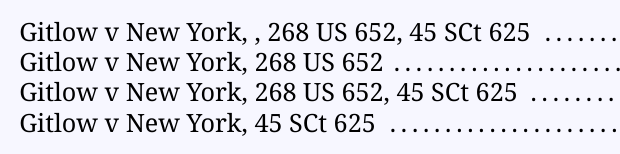
\includegraphics[scale=0.8]{tocexamples.png}}\\
\end{tabular}
\end{center}
\caption[Child keys in the ToC]{For parent-child keys, each unique citation combination results in a separate entry in the Table of Cases. Cite all the children, every time, to get a single entry. Here, the first entry is parent, child1, child2 (\textit{parent has no caseref}); the second and fourth entries are only one child each; and the third, and desired form, is both children. If a partial ref is to be cited, see examples d.\ref{c:indexoffb} or d.\ref{c:indexoffa} for how to switch its indexing off and on.}
\label{fig:indextoc}
\end{figure}



It turns out that one citation command cannot (easily) do all things for all combinations.
\bigskip

The @statute bibentry type is more straightfoward: really, just a title and year in most cases is sufficient.
\bigskip




Both bibentry types will need some additional data (such as shortname) for extra usability.

Note that database entries that look like medium neutral citations (like \textcolor{red}{\lcsetindexingoff\lcrefnn{armstrongmnc}\lcsetindexingon}\footnote{This item has been switched off from being sent to the Table of Cases.}) are stored in the .bib file, and therefore processed by the citation commands, as if they were MNCs, but they will not have internal paragraph numbers or their own page numbers.




\newpage
%\EducNotebook

\def\RotateAngle{180}

\tikzset{
spiral/.pic={
  \draw[rotate=\RotateAngle,
    draw=black,
    left color=black!70,
    right color=black!60,
    middle color=gray!40
    ] 
    (-1.1,-0.35) rectangle ++(10pt,10pt);
  \draw[
    rotate=\RotateAngle,
    double=gray!80,
    double distance=1pt,
    ]
    (-1,-0.2) arc (40:-250:10pt and 2pt);
  \draw[
    rotate=\RotateAngle,
    double=gray!80,
    double distance=1pt,
    ]
    (-1,-0.05) arc (40:-250:10pt and 2pt);
  }
}
%\textwidth = 390pt

      \tikz[remember picture,overlay]
      {
      \draw[rounded corners=10pt,fill=red!1!green!2,drop shadow={shadow xshift=0.5ex, shadow yshift=-0.5ex}]
        ([xshift=-30pt,yshift=20pt]current page text area.north west) rectangle
        ([xshift=30pt,yshift=-20pt]current page text area.south east);
%      \foreach \Valor in {0,1,...,\numexpr\SpiralNumber-1\relax}
%%        \pic at \SpiralPosition {spiral};
        \pic at ([xshift=381pt,yshift=-6em]current page text area.north west) {spiral};
        \pic at ([xshift=381pt,yshift=-12em]current page text area.north west) {spiral};
        \pic at ([xshift=381pt,yshift=-18em]current page text area.north west) {spiral};
        \pic at ([xshift=381pt,yshift=-24em]current page text area.north west) {spiral};
        \pic at ([xshift=381pt,yshift=-30em]current page text area.north west) {spiral};
        \pic at ([xshift=381pt,yshift=-36em]current page text area.north west) {spiral};
        \pic at ([xshift=381pt,yshift=-42em]current page text area.north west) {spiral};
%      \DrawMajorGrid
    \path[clip,rounded corners=10pt]
        ([xshift=-30pt,yshift=20pt]current page text area.north west) rectangle
        ([xshift=30pt,yshift=-20pt]current page text area.south east);
    \draw[black!60,opacity=0.3]
          ([xshift=30pt,yshift=-20pt]current page text area.south east) grid[step=10mm]
          ([xshift=-30pt,yshift=20pt]current page text area.north west);

%      \DrawMinorGrid
    \path[clip,rounded corners=10pt]
        ([xshift=-30pt,yshift=20pt]current page text area.north west) rectangle
        ([xshift=30pt,yshift=-20pt]current page text area.south east);
    \draw[black!20,opacity=0.3]
          ([xshift=30pt,yshift=-20pt]current page text area.south east) grid[step=1mm]
          ([xshift=-30pt,yshift=20pt]current page text area.north west);

      }  

\reversemarginpar
\marginnote{\hl{\textbf{bib} file}}
\normalmarginpar
%%\tikz[remember picture,overlay]
%%      {
%%      \node[xshift=-4em](A){\hl{\textbf{bib} file}}; 
%%      }%
so the bibentry in the \verb|.bib| file will look like: 
%\the\textwidth
\begin{verbatim}
@case{keyabc,
  partya = {ABC}, 
  partyb = {XYZ},
  courtname = {XYZCA},
  casenumber = {456},
  caseyear = {2020},
  reportvolume = {3},
  volyearneeded = {true},
  reportseries = {WLR},
  reportpage = {123},
	}
\end{verbatim}

... and the citation commands:
\bigskip

\mcmd{lawcite}

\mcmd{lcinline}

\mcmd{lcinlinenn}

\mcmd{lcfoot}
\bigskip

... and the component citation commands:
\bigskip

\mcmd{lawcitetitle}

\mcmd{lawciteref}

\mcmd{lcrefnn}

\mcmd{lcnote}

\mcmd{lcshorttitle}

\mcmd{lcnickname}

\bigskip
\setcounter{reftypemode}{1}
\pointing\ \fbox{\lawcite{keyabc}}
\lcsetstyledefault

\newpage


\def\RotateAngle{0}

\tikzset{
spiral/.pic={
  \draw[rotate=\RotateAngle,
    draw=black,
    left color=black!70,
    right color=black!60,
    middle color=gray!40
    ] 
    (-1.1,-0.35) rectangle ++(10pt,10pt);
  \draw[
    rotate=\RotateAngle,
    double=gray!80,
    double distance=1pt,
    ]
    (-1,-0.2) arc (40:-250:10pt and 2pt);
  \draw[
    rotate=\RotateAngle,
    double=gray!80,
    double distance=1pt,
    ]
    (-1,-0.05) arc (40:-250:10pt and 2pt);
  }
}
%\textwidth = 390pt

      \tikz[remember picture,overlay]
      {
      \draw[rounded corners=10pt,fill=red!1!green!2,drop shadow={shadow xshift=0.5ex, shadow yshift=-0.5ex}]
        ([xshift=-30pt,yshift=20pt]current page text area.north west) rectangle
        ([xshift=30pt,yshift=-20pt]current page text area.south east);
%      \foreach \Valor in {0,1,...,\numexpr\SpiralNumber-1\relax}
%%        \pic at \SpiralPosition {spiral};
        \pic at ([xshift=8pt,yshift=-6em]current page text area.north west) {spiral};
        \pic at ([xshift=8pt,yshift=-12em]current page text area.north west) {spiral};
        \pic at ([xshift=8pt,yshift=-18em]current page text area.north west) {spiral};
        \pic at ([xshift=8pt,yshift=-24em]current page text area.north west) {spiral};
        \pic at ([xshift=8pt,yshift=-30em]current page text area.north west) {spiral};
        \pic at ([xshift=8pt,yshift=-36em]current page text area.north west) {spiral};
        \pic at ([xshift=8pt,yshift=-42em]current page text area.north west) {spiral};
%      \DrawMajorGrid
    \path[clip,rounded corners=10pt]
        ([xshift=-30pt,yshift=20pt]current page text area.north west) rectangle
        ([xshift=30pt,yshift=-20pt]current page text area.south east);
    \draw[black!60,opacity=0.3]
          ([xshift=30pt,yshift=-20pt]current page text area.south east) grid[step=10mm]
          ([xshift=-30pt,yshift=20pt]current page text area.north west);

%      \DrawMinorGrid
    \path[clip,rounded corners=10pt]
        ([xshift=-30pt,yshift=20pt]current page text area.north west) rectangle
        ([xshift=30pt,yshift=-20pt]current page text area.south east);
    \draw[black!20,opacity=0.3]
          ([xshift=30pt,yshift=-20pt]current page text area.south east) grid[step=1mm]
          ([xshift=-30pt,yshift=20pt]current page text area.north west);

      }  

%\marginnote{\hl{\textbf{bib} file}}
%\tikz[remember picture,overlay]
%      {
%      \node[xshift=-4em](A){\hl{\textbf{bib} file}}; 
%      }%
for parent-children, the bibentries in the \verb|.bib| file will look like:\marginnote{\hl{parallel\\reports}} 
%\the\textwidth
\bigskip

\rowcolors{1}{}{}

\begin{tabular}{l}
\ttfamily
\makecell[cl]{@case\{armstrong,\tikz[remember picture,overlay]\node(parent){};\\
%\ttfamily
  partya = \bcmd{Adam Armstrong's Case},\\
%\ttfamily
  icaseyear = \bcmd{1823},\\
%\ttfamily
  caseshortname = \bcmd{Armstrong},\\
%\ttfamily
	\}}
\end{tabular}
\smallskip

\begin{tabular}{l}
\ttfamily
@case\{armstrongmnc,\\
\ttfamily
  caseyear = \bcmd{1823},\\
\ttfamily
  courtname = \bcmd{EngR},\\
\ttfamily
  casenumber = \bcmd{1},\\
\ttfamily
  crossref = \bcmd{armstrong},\tikz[remember picture,overlay]\node(child1){};\\
\ttfamily
\}\\
\end{tabular}
\smallskip

\begin{tabular}{l}
\ttfamily
@case\{armstronglewin,\\
\ttfamily
  reportyear = \bcmd{1823},\\
\ttfamily
  reportvolume = \bcmd{1},\\
\ttfamily
  reportseries = \bcmd{Lewin},\\
\ttfamily
  reportpage = \bcmd{245},\\
\ttfamily
  crossref = \bcmd{armstrong},\tikz[remember picture,overlay]\node(child2){};\\
\ttfamily
\}\\
\end{tabular}
\hfill\begin{tabular}{l}
\ttfamily
@case\{armstronger,\\
\ttfamily
  reportvolume = \bcmd{168},\\
\ttfamily
  reportseries = \bcmd{ER},\\
\ttfamily
  reportpage = \bcmd{1028},\\
\ttfamily
  crossref = \bcmd{armstrong},\tikz[remember picture,overlay]\node(child3){};\\
\ttfamily
\}\\
\end{tabular}
\smallskip

\begin{tikzpicture}[remember picture,overlay]
	\path[->, red, thick,bend right=45] (child1.east) edge (parent.east);
	\path[->, red, thick,bend right=60] (child2.east) edge (parent.east);
	\path[->, red, thick,bend right=90] (child3.east) edge (parent.east);
\end{tikzpicture}

... and the citation commands:
\bigskip

%\mcmd{lawcite}

\mcmd{lcinlinerr} \hfill\pointing\ \fbox{\begin{minipage}{0.5\textwidth}\lcinlinerr{armstrongmnc,armstronglewin,armstronger}\end{minipage}}


\mcmd{lcinlinennrr}

\mcmd{lcfootrr}
\bigskip

... and the component citation commands:% (these will retrieve the first key's data fields, except for the citeref command, which will retrieve all the children's caserefs):
\bigskip

\mcmd{lawcitetitlerr}

\mcmd{lawciterefrr}

\mcmd{lcrefnnrr}

\mcmd{lcnoterr}

\mcmd{lcshorttitlerr}

\mcmd{lcnicknamerr}

\rowcolors{1}{blue!7}{blue!7}

\newpage


\subsection{dbx, bbx, cbx, lbx files}

Now, to define the biblatex style (let's call it \verb|lawcite|) that will take that bibentry information and process it.\footnote{The following will just give a general idea of the behind-the-scenes technical structure of the citation mechanism. Examine the actual files for the full details.}
\bigskip

Firstly, a \verb|lawcite.dbx| datamodel file \marginnote{\hl{\textbf{dbx} file}} to make those bibentry fields known to biblatex. Let's make all the fields literals, for the moment.

\begin{verbatim}
\DeclareDatamodelFields[type=field, datatype=literal]{
% case fields
  partya, 
  partyb,
  partysep,
  caseyear, %will be a date
  reportvolume,
  volyearneeded, %will be a boolean
  reportseries,
  reportpage,
  courtname,
  casenumber,
}
\DeclareLanguageMapping{english}{english-lawcite}


\endinput

\end{verbatim}

%\begin{horizon}[mode=unboxed]
%\end{horizon}

Secondly, a \verb|lawcite.bbx| bibliography file \marginnote{\hl{\textbf{bbx} file}} to 
\begin{inparaenum}[\itshape (a)]
\item handle the bibliography formatting, \item define and handle package options being passed in, and \item define and use various utility macros where appropriate\end{inparaenum}. 
Note that bibliographies are not really used in legal work (judgments, professional advice, law review articles, legal essays, and so forth), but some legal style guides do get around to specifying (to varying degrees) how a bibliography, when used, should be laid out and formatted.

In the \verb|.bbx| file, we formally define the new style:

\begin{verbatim}
\ProvidesFile{lawcite.bbx}[2020/04/11 v1.0
        biblatex bibliography style]
\end{verbatim}

and, since legal references are a subset of the authortitle styles (the author being implicit), we can inherit one of those as a base:

\begin{verbatim}
\RequireBibliographyStyle{ext-authortitle-ibid}
\end{verbatim}

Some toggles to keep track of choices: Is the party separator italic? is it dotted? Are the party names italic?:

\begin{verbatim}
%%%%%%%%%
\newtoggle{partysepitalic}
\toggletrue{partysepitalic}
%
\newtoggle{partysepdotted}
\togglefalse{partysepdotted}
%
\newtoggle{partynamesitalic}
\toggletrue{partynamesitalic}
% ...
\end{verbatim}

Name and set the corresponding user options:

\begin{verbatim}
%
\DeclareBibliographyOption[boolean]{party-names-italic}[true]{%
\ifstrequal{#1}{true}
{\toggletrue{partynamesitalic}}
{\togglefalse{partynamesitalic}}%
}
%
\DeclareBibliographyOption[boolean]{party-separator-italic}[true]{%
\ifstrequal{#1}{true}
{\toggletrue{partysepitalic}}
{\togglefalse{partysepitalic}}
}
%
\DeclareBibliographyOption[boolean]{party-separator-dotted}[false]{%
\ifstrequal{#1}{true}
{\toggletrue{partysepdotted}}
{\togglefalse{partysepdotted}}
} ...
\end{verbatim}

Define the bibliography driver for the @case bibentry type. From here on, bibmacros will be used extensively for convenience.

\begin{verbatim}
%
\DeclareBibliographyDriver{case}{%
	\usebibmacro{begentry}
\usebibmacro{getcasenameref}
	\usebibmacro{finentry}
}

\end{verbatim}

Define a sorting templates for cases:

\begin{verbatim}
\DeclareSortingTemplate{casesort}{
\sort{
	\field{partya}
	}
\sort{
	\field{partyb}
	}
\sort{
	\field{caseyear}
	}
\sort{
	\field{reportvolume}
	} 
\sort{
	\field{casenumber}
	} 
\sort{
	\field{reportseries}
	} 
\sort{
	\field{reportpage}
	} 
}
\end{verbatim}

Thirdly, in the citation driver file, \verb|lawcite.cbx|,\marginnote{\hl{\textbf{cbx} file}} where most of the work will be done, we name the citation style and inherit from a pre-existing one:

\begin{verbatim}
\ProvidesFile{lawcite.cbx}[2020-04-11 v1.0
    biblatex citation lawcite style]
\RequireCitationStyle{ext-authortitle-ibid}
\end{verbatim}

Set the formatting of the fields according to the options:

\begin{verbatim}
% fieldformats: case
\DeclareFieldFormat{partya}
{\iftoggle{partynamesitalic}
{\mkbibemph{#1}}{#1}}

\DeclareFieldFormat{partyb}
{\iftoggle{partynamesitalic}
{\mkbibemph{#1}}{#1}}

\DeclareFieldFormat{partysep}{#1}
{\iftoggle{partysepitalic}
{\mkbibemph{#1}{\iftoggle{partysepdotted}
{\adddot}{}}}{#1{\iftoggle{partysepdotted}
{\adddot}{}}}}

...
\end{verbatim}

Some bibmacros:

Note that, if partysep is not a field in the bibentry, it will default to the bibstring \verb|versus|, abbreviation \verb|v|.
 
\begin{verbatim}
% bibmacros

%=========== partysep
\newbibmacro{getpartysep}{%
\iffieldundef{partysep}{%
	\iftoggle{partysepitalic}%
		{\mkbibemph{\bibstring{versus}}}%
		{\bibstring{versus}}%
	\iftoggle{partysepdotted}{\adddot}{}%
	}%
	{%
	\iftoggle{partysepitalic}%
		{\mkbibemph{\printfield{partysep}}}%
		{\printfield{partysep}}%
	\iftoggle{partysepdotted}{\adddot}{}%
	}%
}

%======= casename
\newbibmacro{getcasename}{%
\printfield{partya}%
\iffieldundef{partyb}{}%
{\addspace\usebibmacro{getpartysep}\addspace%
\printfield{partyb}}}%

......

%===== casenameref
\newbibmacro{getcasenameref}{%
	\ifboolexpr{%
		test {\ifcitation}
		and
		test {\ifciteibid}
		}%
		{ibid\addspace}{%
	\usebibmacro{getcasename}%
	\addspace\usebibmacro{getcaseref}
	}%ifciteibid false
} ...
\end{verbatim}

Now, at last, the citation driver.

A citation driver command's structure is:

\begin{verbatim}
\DeclareCiteCommand{xxx}%
{prenote}
{loop; key1, key2, ..., keyn}
{delimiter for multiple keys}
{postnote}
\end{verbatim}

Given that the citation can split into two, the prenote and postnote need to stay with the head and tail, and so are moved into the \textit{loop} parameter\footnote{Meaning that multiple keys do not format correctly in `abovebelow' mode.}, and then a case statement is applied.

\begin{verbatim}
%============= lawcite
\DeclareCiteCommand{lawcite}%
%%caseallabove      reftypemode}{1}}{}
%%caseabovebelow  reftypemode}{2}}{}
%%caseallbelow      reftypemode}{3}}{}
%%casetitleonly     reftypemode}{4}}{}
%%caserefonly       reftypemode}{5}}{}
%@@@@@@@@@@@@@@@@ prenote
{%
	\ifcase\thereftypemode \or%
	\usebibmacro{prenote}%inline
	\or% prenote goes in the footnote for this 
	%variation, along with the case ref.
	\or% prenote is already in the footnote
	\fi%
}% 
%@@@@@@@@@@@@@@@@ item
{%
	\ifcase\thereftypemode%
	\or\usebibmacro{getcasenameref}%
	\or\usebibmacro{getcasename}\footnote{%
	\usebibmacro{prenote}\usebibmacro{getcaseref}\usebibmacro{postnote}}%
	\or\unspace\footnote{\usebibmacro{prenote}%
	\usebibmacro{getcasenameref}\usebibmacro{postnote}}%
	\fi%
%
}%end item
%@@@@@@@@@@@@@@@@ delim
{}%
%@@@@@@@@@@@@@@@@ postnote
{%
	\ifcase\thereftypemode \or%
	\usebibmacro{postnote}% inline
	\or% postnote is already in the footnote
	\or% postnote is already in the footnote
	\fi%
}
\end{verbatim}

And lastly, a language file, \verb|english-lawcite.lbx|, \marginnote{\hl{\textbf{lbx} file}} containing bibstring constants:

\begin{verbatim}
  \ProvidesFile{english-lawcite.lbx}[2019/04/09 
         english with additions for legal citations]
  \InheritBibliographyExtras{english}
  \NewBibliographyString{versus}
  \DeclareBibliographyStrings{%
    inherit   = {english},
    versus = {{versus}{v}},
  }
\endinput
\end{verbatim}

\subsection{Citing}
Text\verb|\lawcite[a prenote][at \mkbibbrackets{45}]{keyabc}| produces:
 
Text\lawcite[a prenote][at \mkbibbrackets{45}]{keyabc}.

%%\section{Additions}
%%We'll add a \verb|\lawcitetitle{}| command to cite just the case name, like this: \lawcitetitle{keyabc}, for refering to in the body of the text.
%%
%%\begin{verbatim}
%%%============= lawcitetitle
%%\DeclareCiteCommand{lawcitetitle}%
%%%@@@@@@@@@@@@@@@@ prenote
%%{\usebibmacro{prenote}}%
%%%@@@@@@@@@@@@@@@@ item
%%{%
%%\usebibmacro{getcasename}%
%%}%end item
%%%@@@@@@@@@@@@@@@@ delim
%%{}%
%%%@@@@@@@@@@@@@@@@ postnote
%%{\usebibmacro{postnote}}
%%\end{verbatim}
%%
%%And a corresponding command \verb|\lawciteref{keyabc}| for the case reference, \lawciteref{keyabc}, so that the following can be done manually: \lawcitetitle{keyabc}\footnote{\lawciteref{keyabc}}.
%%
%%\begin{verbatim}
%%%============= lawciteref
%%\DeclareCiteCommand{lawciteref}%
%%%@@@@@@@@@@@@@@@@ prenote
%%{}%
%%%@@@@@@@@@@@@@@@@ item
%%{%
%%\usebibmacro{prenote}\usebibmacro{getcaseref}\usebibmacro{postnote}%
%%}%end item
%%%@@@@@@@@@@@@@@@@ delim
%%{}%
%%%@@@@@@@@@@@@@@@@ postnote
%%{}
%%\end{verbatim}
%%
%%Now, for law reviews and suchlike, to automate whether, for all citations, the citation is `all below' (in the footnote), or `all above' (as inline text), or the case name above and the case reference below, a counter to act as a switch, and a set of options to set the counter, can be added to the \verb|.bbx| file, and the \verb|\lawcite{}| command modified to take note of the setting and act accordingly. 
%%
%%In the cases \lawcite[prenote2][postnote2]{case2} and \lawcite[prenote3][postnote3]{case3},  and \lawcite[prenote4][postnote4]{case4}  and \lawcite[prenote5][postnote5]{case5} ...
%%
%%And a normal book\autocite[prenoteb1][postnoteb1]{book1}.
%%
%%Text \verb|\lcinline{case3}| produces \\Text \lcinline{case3}, \\
%%Text\verb|\lcfoot{case2}| produces \\
%%Text\lcfoot{case2}.

Some cites\footnote{Chosen randomly: \lcshorttitle{becker} (sarcasm) and \lcshorttitle{columbus} (verse) from the section on humour in \cite[295]{butt}, \lcshorttitle{cassie} from \cite[187]{butt}, on what a ``document'' is, and \lcshorttitle{rmorgan} from \cite[para \mkbibbrackets{8-s 249B.5}, p 1070]{anncrimnsw}, commenting on \lawcite[s 249B(1)]{crimnsw}, Corrupt commissions or rewards: ``If any agent corruptly receives ...'' etc.}:
\begin{inparaenum}[\itshape (a)]\item `The luxuriant growth of this legislative jungle ...'\lcfoot[][29 (Bray CJ)]{becker}. \item ``Dogs will howl and cats will yowl''\lcfootrr{columbussr,columbusne}. \item A video tape is a document\lcfoot{cassie}. \item \textbf{``Receives''} It is not necessary that the agent receives the benefit or reward as an agent\lcfoot{rmorgan}.\end{inparaenum} 

%%\let\opnd\postnotedelim\relax\renewcommand\postnotedelim{\addspace}\lawcite[][xxx(Ohio, Zimmerman J)]{becher}\let\postnotedelim\opnd\relax Text\lawcitefoot[][with postnote]{case2}.

%%Multi-cites: \lawcitesinline{becker,columbussr,cassie,rmorgan}. 
%%
%%\lawcitesinlinerr{thomasermnc, thomascar, thomaser}
%%
%%Multiple keys, one citation: \lcinline{becker,columbussr,cassie,rmorgan}
%%
%%Multiple keys, one citation: \lcinline[prenoteA][postnoteA]{becker,columbussr,cassie,rmorgan}
%%
%%Multi-footcites\lawcitesfoot{becker,columbussr,cassie,rmorgan}. 
%%
%%Single footnote cite\lcfoot{columbussr}.
%%
%%Multi-cites with notes: \lawcitesinline[\note{luxuriant growth}]{becker}[\note{howl\-ing dogs}]{columbussr}[\note{video document}]{cassie}[\note{benefit not as an agent}]{rmorgan}. 
%%
%%
%%``Every idea is an incitement.'' 268 US 652, 673 (1925, New York SC)
%%
%%``Freedom of speech and of the press, as secured by the Constitution, is not an absolute right to speak or publish without responsibility whatever one may choose or an immunity for every possible use of language.''
\begin{quotation}
It is a fundamental principle, long established, that the freedom of speech and of the press which is secured by the Constitution, does not confer an absolute right to speak or publish, without responsibility, whatever one may choose, or an unrestricted and unbridled license that gives immu\-nity for every possible use of language and prevents the punishment of those who abuse this freedom. 2 Story on the Constitution, 5th ed., § 1580, p. 634 -- \lawcitesinlinerr[\nopp 666]{gitlowus}{gitlowsc}.%\lcnote{gitlowsc}.
\end{quotation}

\begin{table}
%\begin{tabular}{l}
%\fbox%\end{tabular}
\end{table}


%%%``the limitations of language'' 57 NY 2d 371, 379
%%%People v. New York Tram Rock Corp., 442 N.E.2d 1222 (N Y 1982)


%Stringed	: \lawcitesinline{becker,becher,cassie} \lawcitesinlinerr{thomasermnc, thomascar, thomaser} \lawcitesinline{columbussr, columbusne}\lawcitesinline{rmorgan}



\noindent ``Certi nomi sono citati da tutti''\footfullcite[110-111]{eco} Some names are cited by everybody.
\bigskip

%%``Dogs will howl'' %	\lcinline[\nopp 200]{columbussr};\lawciteref[\nopp 838]{columbusne}
%%zz\lcnote[pre][post]{book1}zz

%%The capability of having parent (case name) -- child (report ref) relationships between keys, combined with low-level citation commands retrieving specific parts of a reference, allows various combinations of things to be possible.
%%\begin{itemize}
%%\item manually assembled: \lcinlinenn[\nopp 200]{columbussr}; \lcrefnn[\nopp 838]{columbusne} \lcnote[Zimmerman J, for the court]{columbusne}
%%	\begin{itemize}
%%	\item three citation commands, each with its own postnote
%%	\item casenameref\textsuperscript{+\textsc{PN}} + caseref(-note)\textsuperscript{+\textsc{PN}} + note\textsuperscript{+\textsc{PN}}
%%	\end{itemize}
%%\item multicite with multiple keys: \lawcitesinlinerr(Zimmerman J, for the court)[\nopp 200]{columbussr}[\nopp 838]{columbusne}
%%	\begin{itemize}
%%	\item one multicite command with three components
%%	\item postnote + case1key\textsuperscript{+\textsc{PN}} + case2key\textsuperscript{+\textsc{PN}}
%%	\end{itemize}
%%\item multicite with one key: \lawcitesinline(Zimmerman J, for the court)[\nopp 200]{columbussr}
%%	\begin{itemize}
%%	\item postnote + case1key\textsuperscript{+\textsc{PN}}
%%	\end{itemize}
%%\item multicite with one key: \lawcitesinline(Zimmerman J, for the court)[\nopp 838]{columbusne}
%%	\begin{itemize}
%%	\item postnote + case2key\textsuperscript{+\textsc{PN}}
%%	\end{itemize}
%%\item single cite: \lcinline[\nopp 200]{columbussr}, Zimmerman J, for the court
%%	\begin{itemize}
%%	\item case1key\textsuperscript{+\textsc{PN}} + text acting as postnote
%%	\end{itemize}
%%\item single cite: \lcinline[\nopp 838]{columbusne}
%%	\begin{itemize}
%%	\item case2key\textsuperscript{+\textsc{PN}}
%%	\end{itemize}
%%\end{itemize}
%%
%%A multi-key multicite allows individual postnotes for each key:
%%
%%\begin{itemize}
%%	\item \lawcitesinlinerr{armstrongmnc}[\nopp 246]{armstronglewin}[\nopp 1029]{armstronger}
%%	\item \lawcitesinlinerr{alexandermnc}[\nopp 289]{alexandercp}[\nopp 1200]{alexanderer}
%%	\end{itemize}
%%
%%A multi-key single-cite has only one postnote:
%%
%%\begin{itemize}
%%	\item \lcinlinerr[my postnote]{armstrongmnc,armstronglewin,armstronger}
%%	\item \lcinlinerr[A prenote -- see][and another postnote]{alexandermnc,alexandercp,alexanderer}
%%\end{itemize}
%%
%%


The term `common law' is defined by what it is not\footcite[section 41]{bishop}.

Curia Regis
\begin{tabular}{ll}
common law & not statute law \\
common law & not equity \\
common law & not local law\\
common law & not admiralty, probate, etc \\
\end{tabular}

\section{Package Options}
\label{packopt}
Options are processed in sequence, in the order of their appearance in the \texttt{\textbackslash usepackage[$\ldots$]\{biblatex\}} statement, so where there is any overlap, the latter setting will be in effect.
\bigskip

\subsection{Case options}
\optsett{party-names-italic=}{true}
%\noindent\texttt{party-names-italic} \hfill default: \texttt{\textbf{true}}

Sets whether the party names are formatted as italic or as current document format.
\bigskip

\optsett{party-separator-italic=}{true}

Sets whether the separator for the party names (default: v) is formatted as italic or as current document format.
\bigskip

\optsett{party-separator-dotted=}{false}

Sets whether the party separator is dotted (v.) or undotted (v).
\bigskip

\optsett{mnc-brackets=}{true}

Sets whether the caseyear in a Medium Neutral Citation is printed with square brackets, or with just the bare year.
\bigskip

\optsett{casename-comma=}{false}

Sets whether the casename is followed by a comma plus space instead of just a space.
\bigskip

\optsett{multi-comma-sep=}{false}

Sets whether multicites are delimited with a comma plus space instead of semicolon plus space.
\bigskip


\optsett{print-toc-tos=}{true}

Sets whether the Table of Cases and the Table of Statutes is printed or not. The ToC and ToS are actually indexes, and this setting switches the index format to one-column mode for the ToC and ToS.
\bigskip

\optsett{caseref-in-toc=}{true}

Sets whether to print the caseref in the Table of Cases, or not. If true, child entries of a case will print as separate index items (that is, the case name will be repeated). If false, only the casename and the case year (the \texttt{icaseyear} field, for parent-child sets) appear in the ToC.
\bigskip


\subsection{Table of Cases options}

\optsett{comma-in-index=}{true}

Sets whether or not, in the Tables of Cases, a comma is added after the case name for readability.
\bigskip

\optsett{set-lawcite-indexing=}{true}

Sets whether indexing occurs at all. Intended to be used on a per-item basis, to exclude the item when it is part of a set and cited alone. Affects all indexing: ToC, ToS, ToR.
\bigskip


\subsection{Statute options}

\optsett{show-statute-jurisdiction=}{false}

Sets whether or not the statute's jurisdiction, if it exists, should be printed.
\bigskip

\subsection{Table of Statutes/Regulations options}

\optsett{regulations-as-tor=}{true}

Sets whether to print regulations in a separate Table of Regulations (when \textit{true}) or include them in the Table of Statutes (when \textit{false}). Regulations are currently identified via the citeref field of an @statute bibentry pointing to a regulations formatter, or the keywords field containing the `regulations' keyword: \lawcite{testregs}.
\bigskip




\subsection{Citation options}

\optsett{lawrefstyle=}{caseallbelow}

A choice list determining whether the citation with \texttt{\textbackslash lawcite\{\}} prints the citation fully inline (with casename and caseref), fully as a footnote, or with casename inline and caseref as footnote. Intended for (single) citation use in law reviews and legal essays.

The choices are:

\begin{description}
\item[caseallabove] both casename and caseref are inline
\item[caseabovebelow] casename is inline and caseref is in the footnote
\item[caseallbelow] both casename and caseref are in the footnote
\item[casetitleonly] casename appears inline, with pre- and postnote, if any%: \lawcite[pre][post]{becker}
\item[caserefonly] (for future use)
\end{description}


For the first three choices, the prenote of a (single) citation appears with the casename, and the postnote appears with the caseref.
\bigskip


\optsett{lawcitestyle=}{mlr}

A choice list which sets options as a group consistent with a legal citation style guide. For example, the setting, \texttt{mlr} (for \textit{Modern Law Review}), is defined from the option-setting perspective as:

\begin{verbatim}
   party-names-italic=true,
   party-separator-italic=false,
   party-separator-dotted=true,
   lawrefstyle=caseabovebelow,
   print-toc-tos=false,
\end{verbatim}	
	
The built-in choices for lawcitestyle are:

\begin{description}
\item[default] an AGLC-like style
\item[mlr] \textit{Modern Law Review} style
\item[mcgill] McGill style
\end{description}	
	
	
\section{Style-setting commands}
These commands can set or reset a style (or style component) mid-document.

\subsection{Style switching commands}

\optsett{\cmd{lcsetstyledefault}}{}

Set the lawcite style to default citation style. If no lawcite style is specified by the package options or by the other setstyle commands, then the default style is active.
\bigskip
	
\optsett{\cmd{lcsetstylemlr}}{}

Set the lawcite style to \textit{Modern Law Review} citation style. 
\bigskip
	
\optsett{\cmd{lcsetstylemcgill}}{}

Set the lawcite style to McGill citation style. 
\bigskip
	

%\lcsetstyledefault
%\lcsetstylemlr
%\lcsetstylemcgill


\subsection{Style component low-level commands}




\optsett{\cmd{setpartysepitalicon}}{} \\
\optsett{\cmd{setpartysepitalicoff}}{}

Sets whether the party separator string is italic or not.
\bigskip
	

\optsett{\cmd{setpartysepdottedon}}{} \\
\optsett{\cmd{setpartysepdottedoff}}{}

Sets whether the party separator string is dotted or not.
\bigskip
	


\optsett{\cmd{setpartynamesitalicon}}{} \\
\optsett{\cmd{setpartynamesitalicoff}}{}

Sets whether the party names are italic or not.
\bigskip
	




\optsett{\cmd{setmncbracketson}}{} \\
\optsett{\cmd{setmncbracketsoff}}{}

Sets whether the Medium Neutral Citation year is enclosed in square brackets or not.
\bigskip
	


\optsett{\cmd{setprintlegtocon}}{} \\
\optsett{\cmd{setprintlegtocoff}}{}

Sets whether or not to print the Table of Cases.
\bigskip
	


\optsett{\cmd{setrefintocon}}{} \\
\optsett{\cmd{setrefintocoff}}{}

Sets whether to send the caseref to the index, or just the year: \textit{on} = caseref goes to the index; \textit{off} = the year (specifically, the \texttt{caseyear} field, or the \texttt{icaseyear} field of a parent key) goes to the index instead.
\bigskip
	


\optsett{\cmd{setallabove}}{} \\
\optsett{\cmd{setabovebelow}}{} \\
\optsett{\cmd{setallbelow}}{} \\
\optsett{\cmd{settitleonly}}{}

Set the referencing style used by \texttt{\cmd{lawcite}} to: -- fully inline (`allabove'); -- casename inline and caseref footnoted (`abovebelow'); -- fully in the footnote (`allbelow'); or just the casename inline (`titleonly'). 
\bigskip
	
\optsett{\cmd{setstatjurison}}{} \\
\optsett{\cmd{setstatjurisoff}}{}

Sets whether the statute's jurisdiction is printed or not.
\bigskip


\optsett{\cmd{setcasenamecommaon}}{} \\
\optsett{\cmd{setcasenamecommaoff}}{}

Sets whether a comma follows the casename or not.
\bigskip

\optsett{\cmd{setmulticitecommaon}}{} \\
\optsett{\cmd{setmulticitecommaoff}}{}

Sets whether multicites are separated by comma plus space; otherwise, the default delimiter (semicolon plus space) is used.
\bigskip


%\optsett{\cmd{lcnamerefdelim}}{}
%\optsett{\cmd{lcparentchilddelim}}{}

\subsection{Delimiters}


\optsett{\cmd{lcnamerefcommadelim}}{} 

The delimiter (comma plus space) following the casename when the casename-comma option is true.
\bigskip


\optsett{\cmd{statutetitleyeardelim}}{} 

The delimiter between the statute's title and year, defined as a space.
\bigskip

\optsett{\cmd{statutejurisdictiondelim}}{} 

The delimiter before the statute's jurisdiction, defined as a space.



\subsection{Miscellaneous commands}


\optsett{\cmd{setlcinlinecolour\{\}}}{} 

Set the colour of \texttt{\textbackslash lcinline}'s \colorbox{red!10}{\texttt{getcasenameref}} (which may be multiple keys).
\bigskip
	
\optsett{\cmd{setlcinlinerrcolour\{\}}}{} 

Set the colour of \texttt{\textbackslash lcinlinerr}'s first cite key's \colorbox{red!10}{\texttt{getcasenameref}}. %If a Table of Cases is required, the keys for \texttt{\textbackslash lcinlinerr} should generally be all the child keys of a specific parent.
\bigskip
	
\optsett{\cmd{setlcinlinerrcoloursc\{\}}}{} 

Set the colour of \texttt{\textbackslash lcinlinerr}'s second and subsequent cite key's \colorbox{yellow!20}{\texttt{getcaseref}}.
\bigskip

\optsett{\cmd{lcsetindexingoff}}{} \\
\optsett{\cmd{lcsetindexingon}}{}

Switch indexing off and on. Intended for use as a wrapper around an item that is not to go to an index (ToC, ToS, ToR), for example because it is a parent key, or one child key from a child-set.
\bigskip


	

\optsett{\cmd{lcsetdemoon}}{} 

Set demo mode on (e.g., coloured cites).
\bigskip

\optsett{\cmd{lcsetdemooff}}{} 

Set demo mode off.
\bigskip

	
	
	
	
	
	
	
	
\section{Bibmacros}
Besides \texttt{sendtocaseindex} and \texttt{rrindex} for creating the Table of Cases, the following bibmacros (named \textit{get*}) are defined by the package.


%---------------------------------------
\subsection{Bibmacros for Cases}
@case bibentry type:

%\hfill
\begin{tikzpicture}[node distance=20pt,out=0,in=180,relative,scale=0.8]
\node[rectangle,fill=blue!10] (d1) {partya};
\node[rectangle,fill=blue!10,below=of d1] (d2a) {partysep};
\node[rectangle,fill=blue!10,below=of d2a] (d2) {partyb};
\node[rectangle,fill=blue!10,below=of d2] (d3) {caseyear};
\node[rectangle,fill=blue!10,below=of d3] (d4) {courtname};
\node[rectangle,fill=blue!10,below=of d4] (d5) {casenumber};
\node[rectangle,fill=blue!10,below=of d5] (d6) {reportyear};
\node[rectangle,fill=blue!10,below=of d6] (d7) {volyearneeded};
\node[rectangle,fill=blue!10,below=of d7] (d8) {reportvolume};
\node[rectangle,fill=blue!10,below=of d8] (d9) {reportseries};
\node[rectangle,fill=blue!10,below=of d9] (d10) {reportpage};
\node[rectangle,fill=blue!10,below=of d10] (d11) {note};

\node[rectangle,fill=green!20,right=of d2a.east]  (gax) {getpartysep};

\node[rectangle,fill=green!20,right=of d3]               (gb) {getcaseyear};
\node[rectangle,fill=green!20,right=of d4]               (gc) {getcourtname};
\node[rectangle,fill=green!20,right=of d5]               (gd) {getcasenumber};

\node[rectangle,fill=green!20,draw,right=of d6.south east]  (ge) {getreportyear};
\node[rectangle,fill=green!20,right=of d8]               (gf) {getreportvolume};
\node[rectangle,fill=green!20,right=of d9]               (gg) {getreportseries};
\node[rectangle,fill=green!20,right=of d10]              (gh) {getreportpage};

\node[rectangle,fill=green!20,right=of d11]              (gi) {getnote};

\node[rectangle,fill=yellow!20,right=of gax.east]  (ga) {getcasename};
\node[rectangle,fill=yellow!20,right=of gc.north east]  (ha) {getcaseref};
\node[rectangle,fill=yellow!20,right=of gf.south east]  (hb) {getreportref};

\node[rectangle,fill=red!10,right=of ha.south east]  (ia) {getcasenameref};


\path[->, dotted, red, thick] (d2a.east) edge (gax.west);

\path[->, red, thick,bend left=45] (d1.east) edge (ga.north west);
\path[->, red, thick,bend right=30] (d2.east) edge (ga.south west);
\path[->, red, thick] (gax) edge (ga);
\path[->, red, thick] (d3) edge (gb);
\path[->, red, thick] (d4) edge (gc);
\path[->, red, thick] (d5) edge (gd);
%\draw[->] (d1) -- (ga);
%\draw[->] (d2) -- (ga);
%\draw[->] (d3) -- (gb);
%\draw[->] (d4) -- (gc);
%\draw[->] (d5) -- (gd);

\path[->, red, thick,bend left=45] (d6.east) edge (ge.north west);
\path[->, red, thick,bend right=45,out=0,in=180] (d7.north) edge (ge.south west);
\path[->, red, thick] (d8) edge (gf);
\path[->, red, thick] (d9) edge (gg);
\path[->, red, thick] (d10) edge (gh);
%\draw[->] (d6)  -- (ge);
%\draw[->] (d7)  -- (ge);
%\draw[->] (d8)  -- (gf);
%\draw[->] (d9)  -- (gg);
%\draw[->] (d10) -- (gh);

\draw[->, red, thick] (d11) -- (gi);

\path[->, red, thick,bend left=45] (ga.east) edge (ia.north);
%\draw[->] (ga) -- (ia);
\path[->, red, thick,bend left=45] (gb.east) edge (ha.north);
\path[->, red, thick] (gc.east) edge (ha.west);
\path[->, red, thick,bend right=45] (gd.east) edge (ha.south);
%\draw[->] (gb) -- (ha);
%\draw[->] (gc) -- (ha);
%\draw[->] (gd) -- (ha);


\draw[->, red, thick] (ge) -- (hb);
\draw[->, red, thick] (gf) -- (hb);
\draw[->, red, thick] (gg) -- (hb);
\draw[->, red, thick] (gh) -- (hb);

\path[->, red, thick,bend right=70] (gi.east) edge (ia.south);
%\draw[->] (gi) -- (ia);
\draw[->, red, thick] (ha) -- (ia);
\draw[->, red, thick] (hb) -- (ia);

%MNC:
\node[ right=of d3.north east,xshift=-1em] (d3x) {};
\node[ left=of d5.south west,xshift=2em] (d5x) {};
\draw[blue, thick, behind path]  (d5x.south west) rectangle (d3x.north east);

\end{tikzpicture}
%\hfill\ 
\bigskip

Additional fields:

\begin{tikzpicture}[node distance=20pt,out=0,in=180,relative,scale=0.8]
\node[rectangle,fill=blue!10] (add1) {caseshortname};
\node[rectangle,fill=green!20,right=of add1] (add2) {getcaseshortname};
\draw[->, red, thick] (add1) -- (add2);
\node[rectangle,fill=blue!10,below=of add1] (add3) {casenickname};
\node[rectangle,fill=green!20,right=of add3] (add4) {getcasenickname};
\draw[->, red, thick] (add3) -- (add4);
\end{tikzpicture}
\bigskip



%---------------------------------------
\subsection{Bibmacros for Statutes}
@statute bibentry type:

\begin{tikzpicture}[node distance=20pt,out=0,in=180,relative,scale=0.8]
\node[rectangle,fill=blue!10] (stata) {statutetitle};
\node[rectangle,fill=blue!10,below=of stata] (statb) {statutetitleyear};
\node[rectangle,fill=blue!10,below=of statb] (statc) {statutejurisdiction};

\node[rectangle,fill=green!20,right=of stata] (statka) {getstatutetitle};
\node[rectangle,fill=green!20,right=of statc] (statkc) {getstatutejurisdiction};

\node[rectangle,fill=yellow!20,below=of statka,xshift=6em] (statmc) {getstatutename};

\draw[->, red, thick] (stata) -- (statka);
\draw[->, red, thick] (statb) -- (statka);
\draw[->, red, thick] (statc) -- (statkc);

\draw[->, red, thick] (statka) -- (statmc);
\draw[->, red, thick] (statkc) -- (statmc);

\node[rectangle,fill=red!10,right=of statmc] (statnc) {getstatutenameref};

\draw[->, red, thick] (statmc) -- (statnc);

\end{tikzpicture}
\bigskip




%---------------------------------------
\subsection{Bibmacros for Law Journals}
@article bibentry type:


\begin{tikzpicture}[node distance=20pt,out=0,in=180,relative,scale=0.8]
\node[rectangle,fill=blue!10] (lja) {author};
\node[rectangle,fill=blue!10,below=of lja] (ljb) {title};
\node[rectangle,fill=blue!10,below=of ljb] (ljc) {subtitle};
\node[rectangle,fill=blue!10,below=of ljc] (ljd) {year};
\node[rectangle,fill=blue!10,below=of ljd] (lje) {volume};
\node[rectangle,fill=blue!10,below=of lje] (ljf) {journaltitle};
\node[rectangle,fill=blue!10,below=of ljf] (ljg) {pages};
\node[rectangle,fill=blue!10,below=of ljg] (ljgg) {related};

\node[rectangle,fill=green!20,right=of lja] (lka) {getljarticleauthor};
\node[rectangle,fill=green!20,right=of ljb] (lkb) {getljarticletitle};
%\node[rectangle,fill=green!20,right=of ljb] (ljc) {subtitle};
\node[rectangle,fill=green!20,right=of ljd] (lkd) {getljarticleyear};
\node[rectangle,fill=green!20,right=of lje] (lke) {getljarticlevolume};
\node[rectangle,fill=green!20,right=of ljf] (lkf) {getljarticlejournaltitle};
\node[rectangle,fill=green!20,right=of ljg] (lkg) {getljarticlepage};
\node[rectangle,fill=green!20,right=of ljgg] (lkgg) {related};

\draw[->, red, thick] (lja) -- (lka);
\draw[->, red, thick] (ljb) -- (lkb);
\draw[->, red, thick] (ljc.north) -- (lkb.south west);
\draw[->, red, thick] (ljd) -- (lkd);
\draw[->, red, thick] (lje) -- (lke);
\draw[->, red, thick] (ljf) -- (lkf);
\draw[->, red, thick] (ljg) -- (lkg);
\draw[->, red, thick] (ljgg) -- (lkgg);

\node[rectangle,              right=of lkd,xshift=4em]  (ljh) {         };
\node[rectangle,fill=red!10,right=of ljh]  (lkh) {getljarticle};


\path[->, red, thick,bend left=70] (lka.east) edge (lkh.north);
\path[->, red, thick,bend left=40] (lkb.east) edge (lkh.north);
\path[->, red, thick                ] (lkd.east) edge (lkh.west);
\path[->, red, thick,bend right=30] (lke.east) edge (lkh.south);
\path[->, red, thick,bend right=50] (lkf.east) edge (lkh.south);
\path[->, red, thick,bend right=70] (lkg.east) edge (lkh.south);
\path[->, red, thick,bend right=82] (lkgg.east) edge (lkh.south);


%\node[rectangle,fill=green!20,right=of add1] (add2) {getcaseshortname};
%\draw[->, red, thick] (add1) -- (add2);
%\node[rectangle,fill=blue!10,below=of add1] (add3) {casenickname};
%\node[rectangle,fill=green!20,right=of add3] (add4) {getcasenickname};
%\draw[->, red, thick] (add3) -- (add4);
\end{tikzpicture}
\bigskip



\section{Citation Commands}
\subsection{The \textbackslash lawcite Command}
The \texttt{\textbackslash lawcite} command is style-sensitive.

With current settings, \texttt{\textbackslash lawcite} produces:\marginnote{\refstepcounter{democount}(d.\thedemocount)\label{c:norm}}
\begin{filecontents}[overwrite,nosearch,noheader]{\democodefile}
Text\lawcite{becker}\\
Text\lawcite{columbusne}
\end{filecontents}
\PrintDemo {style=parallel}
\bigskip
\hfill * \hfill\ 
\bigskip

Swapping to mlr style:\marginnote{\refstepcounter{democount}(d.\thedemocount)\label{c:mlr}}


\begin{filecontents}[overwrite,nosearch,noheader]{\democodefile}
\lcsetstylemlr
\lawcite{becker}\\
\lawcite{columbusne}
\lcsetstyledefault
\end{filecontents}
\PrintDemo {style=parallel}
\bigskip
\hfill * \hfill\ 
\bigskip


%See d.\ref{c:norm}5



Multiple keys are handled in `abovebelow' mode:\marginnote{\refstepcounter{democount}(d.\thedemocount)\label{c:mab}}
\begin{filecontents}[overwrite,nosearch,noheader]{\democodefile}
\setcounter{reftypemode}{2}
\lawcite{becker,rmorgan}
\end{filecontents}
\PrintDemo {style=parallel}
\bigskip
\hfill * \hfill\ 
\bigskip

Multiple keys in `allabove' mode are also typeset correctly:
\marginnote{\refstepcounter{democount}(d.\thedemocount)\label{c:maa}}
\begin{filecontents}[overwrite,nosearch,noheader]{\democodefile}
\setcounter{reftypemode}{1}
\lawcite{becker,rmorgan}
\end{filecontents}
\PrintDemo {style=parallel}
\bigskip
\hfill * \hfill\ 
\bigskip

However, multiple keys in `allbelow' mode are not handled well - use \texttt{\textbackslash lcfoot} instead (see example d.\ref{c:lcfoot}):
\marginnote{\refstepcounter{democount}(d.\thedemocount){\color{red}*}\label{c:mallb}}
\begin{filecontents}[overwrite,nosearch,noheader]{\democodefile}
\setcounter{reftypemode}{3}
Text\lawcite{becker,rmorgan}
\end{filecontents}
\PrintDemo {style=parallel}
\bigskip
\hfill * \hfill\ 
\bigskip


Parallel reports `allabove' - use \texttt{\textbackslash lcinlinerr} instead (see example d.\ref{c:lcinlinerr}):\marginnote{\refstepcounter{democount}(d.\thedemocount){\color{red}*}}
\begin{filecontents}[overwrite,nosearch,noheader]{\democodefile}
\setcounter{reftypemode}{1}
\lawcite{columbussr,columbusne}
\end{filecontents}
\PrintDemo {style=parallel}
\bigskip
\hfill * \hfill\ 
\bigskip


Parallel reports `abovebelow' - only usable if refferring to the reports as individual items:\marginnote{\refstepcounter{democount}(d.\thedemocount){\color{red}*}}
\begin{filecontents}[overwrite,nosearch,noheader]{\democodefile}
\setcounter{reftypemode}{2}
\lawcite{columbussr,columbusne}
\end{filecontents}
\PrintDemo {style=parallel}
\bigskip
\hfill * \hfill\ 
\bigskip


Parallel reports `allbelow'  - use \texttt{\textbackslash lcfootrr} instead (see example d.\ref{c:lcfoot}):\marginnote{\refstepcounter{democount}(d.\thedemocount){\color{red}*}}
\begin{filecontents}[overwrite,nosearch,noheader]{\democodefile}
\setcounter{reftypemode}{3}
Text\lawcite{columbussr,columbusne}
\end{filecontents}
\PrintDemo {style=parallel}
\bigskip
\hfill * \hfill\ 
\bigskip

\lcsetstyledefault %back to `normal'

Statutes:\marginnote{\refstepcounter{democount}(d.\thedemocount)\label{c:statute}}
\begin{filecontents}[overwrite,nosearch,noheader]{\democodefile}
\lawcite{crimnsw}
\end{filecontents}
\PrintDemo {style=parallel}
\bigskip
\hfill * \hfill\ 
\bigskip



\subsection{Cases}
\subsubsection{Citing a Component}

Citing the case name only:\marginnote{\refstepcounter{democount}(d.\thedemocount)}
\begin{filecontents}[overwrite,nosearch,noheader]{\democodefile}
\lawcitetitle{becker}\\
\lawcitetitlerr{columbussr,columbusne}
\end{filecontents}
\PrintDemo {style=parallel}
\bigskip
\hfill * \hfill\ 
\bigskip


Citing the case reference only:\marginnote{\refstepcounter{democount}(d.\thedemocount)}
\begin{filecontents}[overwrite,nosearch,noheader]{\democodefile}
\lawciteref{becker}\\
\lawciteref{columbussr,columbusne}
\end{filecontents}
\PrintDemo {style=parallel}
\bigskip
\hfill * \hfill\ 
\bigskip



Citing the case reference, without the note:\marginnote{\refstepcounter{democount}(d.\thedemocount)}
\begin{filecontents}[overwrite,nosearch,noheader]{\democodefile}
\lcrefnn{becker}\\
\lcrefnnrr{columbussr,columbusne}
\end{filecontents}
\PrintDemo {style=parallel}
\bigskip
\hfill * \hfill\ 
\bigskip


Citing the note only:\marginnote{\refstepcounter{democount}(d.\thedemocount)}
\begin{filecontents}[overwrite,nosearch,noheader]{\democodefile}
\lcnote{becker}\\
\lcnoterr{columbussr,columbusne}
\end{filecontents}
\PrintDemo {style=parallel}
\bigskip
\hfill * \hfill\ 
\bigskip


Citing the case shortname only:\marginnote{\refstepcounter{democount}(d.\thedemocount)}
\begin{filecontents}[overwrite,nosearch,noheader]{\democodefile}
\lcshorttitle{becker}\\
\lcshorttitlerr{columbussr,columbusne}\\
\lcshorttitlerr{gitlowus,gitlowsc}
\end{filecontents}
\PrintDemo {style=parallel}
\bigskip
\hfill * \hfill\ 
\bigskip


\subsubsection{Single-cite, multi-keys}

Citing unrelated keys inline:\marginnote{\refstepcounter{democount}(d.\thedemocount)}
\begin{filecontents}[overwrite,nosearch,noheader]{\democodefile}
\lcinline{becker,cassie}\\
\lcinline{columbusne,gitlowus}
\end{filecontents}
\PrintDemo {style=parallel}
\bigskip
\hfill * \hfill\ 
\bigskip

Citing child keys inline:\marginnote{\refstepcounter{democount}(d.\thedemocount)\label{c:lcinlinerr}}
\begin{filecontents}[overwrite,nosearch,noheader]{\democodefile}
\lcinlinerr{alexandermnc,alexandercp,alexanderer}\\
\lcinlinerr{columbussr,columbusne}
\end{filecontents}
\PrintDemo {style=parallel}
\bigskip
\hfill * \hfill\ 
\bigskip


Citing inline, without the note:\marginnote{\refstepcounter{democount}(d.\thedemocount)}
\begin{filecontents}[overwrite,nosearch,noheader]{\democodefile}
\lcinlinenn{becker}\\
\lcinlinennrr{columbussr,columbusne}
\end{filecontents}
\PrintDemo {style=parallel}
\bigskip
\hfill * \hfill\ 
\bigskip


%%%Citing the case as a footnote only:\marginnote{\refstepcounter{democount}(d.\thedemocount)*}
%%%\begin{filecontents}[overwrite,nosearch,noheader]{\democodefile}
%%%Text\lawcitefoot[See][both on topic]{becker,cassie}\\
%%%Text\lawcitefoot{columbusne}
%%%\end{filecontents}
%%%\PrintDemo {style=parallel}
%%%\bigskip
%%%\hfill * \hfill\ 
%%%\bigskip


Citing the case as a footnote:\marginnote{\refstepcounter{democount}(d.\thedemocount)\label{c:lcfoot}}
\begin{filecontents}[overwrite,nosearch,noheader]{\democodefile}
Text\lcfoot[See][both on topic]{becker,cassie}\\
Text\lcfootrr{columbussr,columbusne}
\end{filecontents}
\PrintDemo {style=parallel}
\bigskip
\hfill * \hfill\ 
\bigskip


\subsubsection{Multicite commands: single cite and multicite: multi-keys}

Citing unrelated multiple keys inline:\marginnote{\refstepcounter{democount}(d.\thedemocount)}
\begin{filecontents}[overwrite,nosearch,noheader]{\democodefile}
\lawcitesinline{becker,rmorgan,cassie}\\
\lawcitesinline{columbusne,alexandermnc}
\end{filecontents}
\PrintDemo {style=parallel}
\bigskip
\hfill * \hfill\ 
\bigskip

Citing unrelated multiple keys, with multicites, inline:\marginnote{\refstepcounter{democount}(d.\thedemocount)}
\begin{filecontents}[overwrite,nosearch,noheader]{\democodefile}
\lawcitesinline[\nopp 15]{becker}[\nopp 1055]{rmorgan}[\mkbibbrackets{21}]{cassie}\\
\lawcitesinline[\nopp 838]{columbusne}[\nopp 1201]{alexanderer}
\end{filecontents}
\PrintDemo {style=parallel}
\bigskip
\hfill * \hfill\ 
\bigskip


Citing child multi-keys inline:\marginnote{\refstepcounter{democount}(d.\thedemocount)}
\begin{filecontents}[overwrite,nosearch,noheader]{\democodefile}
\lawcitesinlinerr[See also][]{armstrongmnc,armstronglewin,armstronger}\\
\lawcitesinlinerr{columbussr, columbusne}
\end{filecontents}
\PrintDemo {style=parallel}
\bigskip
\hfill * \hfill\ 
\bigskip


Citing child multi-keys inline, with multicites:\marginnote{\refstepcounter{democount}(d.\thedemocount)}
\begin{filecontents}[overwrite,nosearch,noheader]{\democodefile}
\lawcitesinlinerr(See also)(){armstrongmnc}[\nopp 247]{armstronglewin}[\nopp 1029]{armstronger}\\
\lawcitesinlinerr[\nopp 200]{columbussr}[\nopp 838]{columbusne}
\end{filecontents}
\PrintDemo {style=parallel}
\bigskip
\hfill * \hfill\ 
\bigskip


Citing unrelated multiple keys in the footnote:\marginnote{\refstepcounter{democount}(d.\thedemocount)\label{c:indexoffb}}
\begin{filecontents}[overwrite,nosearch,noheader]{\democodefile}
Text\lawcitesfoot[See also][all examining the matter]{becker,cassie,rmorgan}\\
\lcsetindexingoff%Do not send to ToC
Text\lawcitesfoot{columbusne,armstrongmnc}
\lcsetindexingon
\end{filecontents}
\PrintDemo {style=parallel}
\bigskip
\hfill * \hfill\ 
\bigskip

Citing unrelated multiple keys, with multicites, in the footnote:\marginnote{\refstepcounter{democount}(d.\thedemocount)\label{c:indexoffa}}
\begin{filecontents}[overwrite,nosearch,noheader]{\democodefile}
Text\lawcitesfoot(See also)(all examining the matter)[\nopp 21]{becker}[\mkbibbrackets{15}]{cassie}[\nopp 1055]{rmorgan}\\
\lcsetindexingoff%Do not send to ToC
Text\lawcitesfoot[\nopp 838]{columbusne}[\nopp 247]{armstronglewin}
\lcsetindexingon
\end{filecontents}
\PrintDemo {style=parallel}
\bigskip
\hfill * \hfill\ 
\bigskip


Citing child multi-keys, with multicites, in the footnote:\marginnote{\refstepcounter{democount}(d.\thedemocount)}
\begin{filecontents}[overwrite,nosearch,noheader]{\democodefile}
Text\lawcitesfootrr[\nopp 198]{columbussr}[\nopp 838]{columbusne}
\end{filecontents}
\PrintDemo {style=parallel}
\bigskip
\hfill * \hfill\ 
\bigskip

\subsubsection{Demo Mode}


Demo mode on:
\begin{filecontents}[overwrite,nosearch,noheader]{\democodefile}
\lcsetdemoon
\lcinlinerr{columbussr, columbusne}\\
\lcinline{becker,cassie}\\
Text\lcfootrr{columbussr, columbusne}
\end{filecontents}
\PrintDemo {style=parallel}
\bigskip
\hfill * \hfill\ 
\bigskip


Demo mode off:
\begin{filecontents}[overwrite,nosearch,noheader]{\democodefile}
\lcsetdemooff
\lcinlinerr{columbussr, columbusne}\\
\lcinline{becker,cassie}\\
Text\lcfootrr{columbussr, columbusne}
\lcsetdemoon
\end{filecontents}
\PrintDemo {style=parallel}
\bigskip
\hfill * \hfill\ 
\bigskip


\subsection{Statutes}
The \verb|\lawcite| command (see example d.\ref{c:statute}) does generic statute citation.

It can also do specific-style formatting as provided by the \verb|citeref={}| mechanism, such as this old Alberta regulation about elevating devices: \marginnote{\refstepcounter{democount}(d.\thedemocount)}
\begin{filecontents}[overwrite,nosearch,noheader]{\democodefile}
\lawcite{canregalta}
\end{filecontents}
\PrintDemo {style=parallel}
where \verb|\lawcite| is acting as a despatcher to a case statement of the type \texttt{\textbackslash iffieldequalstr\{citeref\}\{altareg\}} and the bibentry looks like this:
\begin{verbatim}
@statute{canregalta,
citeref = {altareg},
year = {2009},
regnum = {62},
}
\end{verbatim}
\bigskip
\hfill * \hfill\ 
\bigskip


\lawcite[\bibstring{section} 9 \mkbibparens{1955}]{canreg}: ``Maple syrup shall be packed as required by this Part [=Part II -- Packing] as a condition to application or use of a grade name in respect of that syrup.''
\bigskip

Helper macros for use in the postnote are provided to make referring to bibstrings (section, sections) easier.
\bigskip

{\small\noindent
\begin{tabular}{ll}
Postnote Macro & Typesets as \\
\cmd{lcsec}\braces{9} & \canreg{canreg}{\textcolor{red}{\lcsec{9}}} \\
\cmd{lcsecyr}\braces{9}\braces{1955} & \canreg{canreg}{\textcolor{red}{\lcsecyr{9}{1955}}} \\
\cmd{lcssec}\braces{9-10} & \canreg{canreg}{\textcolor{red}{\lcssec{9-10}}} \\
\cmd{lcssecyr}\braces{9-10}\braces{1955} & \canreg{canreg}{\textcolor{red}{\lcssecyr{9-10}{1955}}} \\
no pinpoint & \canreg{canreg}{} \\
\end{tabular}
}
\bigskip

\rowcolors{1}{blue!5}{blue!9}

The formats of Canadian regulations are pre-defined in the package\footnote{According to AGLC3 style advice.}. An @statute bibentry with the \texttt{citeref=\{crcreg\}} field will be sent by \texttt{\cmd{lawcite}} to the appropriate Canadian regulation citation formatter for CRC regulations, \verb|altareg| will go to Alta Reg, and so on.
\bigskip

Citeref values for Canadian regulations:
\bigskip

\begin{tabular}{ll}
...reg & Example of format (from AGLC3)\\
crc & \lawcite{canregcrc} \\
sor & \lawcite{canregsor} \\
alta & \lawcite{canregalta} \\
bc & \lawcite{canregbc} \\
man & \lawcite{canregman} \\
nb & \lawcite{canregnb} \\
nfld & \lawcite{canregnfld} \\
nlr & \lawcite{canregnlr} \\
nwt & \lawcite{canregnwt} \\
ns & \lawcite{canregns} \\
nu & \lawcite{canregnu} \\
o & \lawcite{canrego} \\
pei & \lawcite{canregpei} \\
qc & \lawcite{canregoc} \\
sask & \lawcite{canregsask} \\
yoic & \lawcite{canregyoic} \\
\end{tabular}
\bigskip

The bibentry data fields required by the various Canadian regulation types are:
\bigskip

\begin{tabular}{lllllll}
crc & title & chapter &&&& \\
sor & title && year & regnum && \\
alta & && year & regnum && \\
bc &  && year & regnum && \\
man & && year & regnum && \\
nb &  && year & regnum && \\
nfld &  && year & regnum && \\
nlr &  && year & regnum && \\
nwt &  && year & regnum && \\
ns &  && year & regnum && \\
nu &  && year & regnum && \\
o &  && year & regnum && \\
pei &  && year & regnum && \\
qc &  && year & regnum & fulldate & gazette\\
sask &  && year & regnum && \\
yoic &  && year & regnum && \\
\end{tabular}

\bigskip

Australian regulations look like statutes and can be cited like them.
\bigskip

\hfill * \hfill\ 
\bigskip

``In the Canadian jurisdictions, 
\lawcite[\lcsec{25}]{canleg} and 
\lawcite[\lcsec{515}]{crimcodecan} and
\lawcite{oescheats} apply.''
\bigskip

For Canadian statutes, the citeref value is \verb|canleg| and requires title, chapter and svjy (statute volume, jurisdiction, year) fields in the bibentry:
\bigskip

\begin{tabular}{llll}
canleg & title & svjy & chapter \\
\end{tabular}
\bigskip

\begin{verbatim}
@statute{canleg,
citeref = {canleg},
title = {Copyright Act},
chapter = {C-42},
svjy = {RSC 1985},
}
\end{verbatim}



\section{Multicite Usage}
This section illustrates the use of multicite commands for cases, in particular, how the prenote(s) and postnote(s) work.

Multicite commands can do a single cite of a group of one or more keys, with a prenote and a postnote bracketing the group:

\begin{center}
\colorbox{yellow!12}{$e$ $C_1$; $C_2$; $C_3$, $o$}
\end{center}

Alternatively, a multicite command can do multicites, placing a prenote and postnote around each key in the group:

\begin{center}
\colorbox{yellow!12}{$e_a$ $C_1$, $o_a$; $e_b$ $C_2$, $o_b$; $e_c$ $C_3$, $o_c$}
\end{center}

The synax is different for each method.

The multicite commands are: 
\begin{itemize}
\item[] \verb|\lawcitesinline|, for inline unrelated reports
\item[] \verb|\lawcitesinlinerr|, for inline reports of the same case
\item[] \verb|\lawcitesfoot|, for footnote unrelated reports
\item[] \verb|\lawcitesfootrr|, for footnote reports of the same case
\end{itemize}


\subsection{Multiple Keys}
\subsubsection{Separate Cases}
A string of authorities\marginnote{% 
\begin{tikzpicture}[node distance=7pt]
\node[circle] (Ca) {\small $C_a$};
\node[circle,right=of Ca,xshift=-1.5em] (Cb) {\small $C_b$};
\node[circle,right=of Cb,xshift=-1.5em] (Cc) {\small $C_c$};
\node[rectangle,below=of Ca] (r1) {\small $r_1$};
\node[rectangle,below=of Cb] (r2) {\small $r_2$};
\node[rectangle,below=of Cc] (r3) {\small $r_3$};
\draw [->] (Ca) -- (r1);
\draw [->] (Cb) -- (r2);
\draw [->] (Cc) -- (r3);
\end{tikzpicture}
} can be cited in one citation, as a block, with a prenote and postnote around the whole lot, or multi-cited with individual prenotes and postnotes.

The citation command retrieves \texttt{casenameref} for each key in the citation.
\bigskip

\noindent
\theball
multiciting: different cases, single cite: \\
\verb|\lawcitesinline|
\bigskip

%%%output:
%%%
%%%\begin{mdframed}[style=default]
%%%\lawcitesinline[prenoteA][postnoteB]{becker,columbussr,cassie,rmorgan}
%%%\end{mdframed}
%%%\bigskip
%%%
%%%syntax:
%%%
%%%%----------------------
%%%\begin{mdframed}[style=syntax]
%%%\textbackslash lawcitesinline [prenoteA] [postnoteB] \{\displaykey{becker}, \displaykey{columbussr}, \displaykey{cassie}, \displaykey{rmorgan}\}
%%%\end{mdframed}
%%%%----------------------

\renewcommand\democodeprefix{{\small syntax:} }
\renewcommand{\demoresultprefix}{\noindent {\small output:}}
%%\renewenvironment{latexresult}{%
%%\demoresultprefix
%%\nopagebreak[4]
%%\preResultSkip
%%\mdframed[%
%%style=syntax,
%%%backgroundcolor=demo@resultbackcolor,%
%%usetwoside=false,
%%]%
%%}{
%%\endmdframed
%%\noindent
%%}
%%%

%%%\lstdefinestyle{lstDemoStyleLaTeXCode}{ %
%%%%%% base style
%%%,style=lstDocStyleBase
%%%%%% Line numbers
%%%,numbers=none % left, right, none
%%%%%% colors
%%%,stringstyle=\color{blue}
%%%,keywordstyle=\color{blue}
%%%,commentstyle=\color{brown}
%%%,backgroundcolor=\color{yellow!40}%white}
%%%,rulecolor=\color{black}
%%%%%% frame
%%%,frame=shadowbox % none, leftline, topline, bottomline, lines
%%%% single, shadowbox
%%%,framesep=3pt
%%%,rulesep=2pt % control the space between frame and listing
%%%% and between double rules.
%%%,framerule=0.4pt % controls the width of the rules.
%%% }

\begin{filecontents}[overwrite,nosearch,noheader]{\democodefile}
\lawcitesinline[prenoteA][postnoteB]{becker,columbussr,cassie,rmorgan}
\end{filecontents}
\PrintCodeAndResultsStackedR
%----------------------
%\vspace*{0.5em}\par%\noindent
%\printlatexresult%
%\par%\noindent
%\democodeprefix
%\begin{mdframed}[style=syntax]
%\lstinputlisting[basicstyle=\rmfamily]{\democodefile}
%\end{mdframed}
%----------------------
%yyy

\spotsep


\noindent
\theball
multiciting: different cases, multi-cites: \\
\verb|\lawcitesinline|
\bigskip

%%output:
%%
%%\begin{mdframed}[style=default]
%%\lawcitesinline[prenoteA][postnoteB]{becker}[prenoteC][postnoteD]{columbussr}[prenoteE][postnoteF]{cassie}[prenoteG][postnoteH]{rmorgan}
%%\end{mdframed}
%%\bigskip
%%
%%syntax:
%%
%%%----------------------
%%\begin{mdframed}[style=syntax]
%%\textbackslash lawcitesinline [prenoteA] [postnoteB] \{\displaykey{becker}\} [prenoteC] [postnoteD] \{\displaykey{columbussr}\} [prenoteE] [postnoteF] \{\displaykey{cassie}\} [prenoteG] [postnoteH] \{\displaykey{rmorgan}\}
%%\end{mdframed}
%----------------------
\begin{filecontents}[overwrite,nosearch,noheader]{\democodefile}
\lawcitesinline[prenoteA][postnoteB]{becker}[prenoteC][postnoteD]{columbussr}[prenoteE][postnoteF]{cassie}[prenoteG][postnoteH]{rmorgan}
\end{filecontents}
\PrintCodeAndResultsStackedR

\setlcinlinecolour{green}Use \verb|\setlcinlinecolour{green}| to:

\begin{filecontents}[overwrite,nosearch,noheader]{\democodefile}
\lawcitesinline[prenoteA][postnoteB]{becker}[prenoteC][postnoteD]{columbussr}[prenoteE][postnoteF]{cassie}[prenoteG][postnoteH]{rmorgan}
\end{filecontents}
\PrintCodeAndResultsStackedR
\setlcinlinecolour{red}

\spotsep

\subsubsection{One Case: Parent-Child Keys with \texttt{crossref}}
With one case and multiple reports, the casename only needs to be shown once, followed by a string of case references.\marginnote{% 
\begin{tikzpicture}[node distance=5pt]
\node[circle] (C) {\small $C_a$};
\node[rectangle,below=of C] (r1) {\small $r_1$};
\node[rectangle,right=of r1] (r2) {\small $r_2$};
\node[rectangle,right=of r2] (r3) {\small $r_3$};
\draw [->] (C) -- (r1);
\draw [->] (C) -- (r2);
\draw [->] (C) -- (r3);
\end{tikzpicture}
}

This is handled by using a parent key with two or more child keys, each child key being one law report.

A parent key (never cited) holds the party names and nothing more, and each child inherits all fields from the parent when the child entry has a \texttt{crossref=\{parentkey\},} field. The child keys explicitly store only the caseref, with the casename coming from the parent.

The citation command handles the assembly of the citation by using the \texttt{\textbackslash iffirstcitekey\{\textbf{true}\}\{\textbf{false}\}} test: the first child retrieves \texttt{casenameref}, and the other children retrieve only \texttt{caseref}.
\bigskip

\noindent
\theball
multiciting: same case, different reports, single cite: \\
\verb|\lawcitesinlinerr|
\bigskip

%%%output:
%%%
%%%\begin{mdframed}[default]
%%%\lawcitesinlinerr[prenoteA][postnoteB]{columbussr, columbusne}
%%%\end{mdframed}
%%%\bigskip
%%%
%%%syntax:
%%%
%%%%----------------------
%%%\begin{mdframed}[style=syntax]
%%%\textbackslash lawcitesinlinerr [prenoteA] [postnoteB] \{\displaykey{columbussr}, \\ \displaykey{columbusne}\}
%%%\end{mdframed}
%%%%----------------------
\begin{filecontents}[overwrite,nosearch,noheader]{\democodefile}
\lawcitesinlinerr[prenoteA][postnoteB]{columbussr, columbusne}
\end{filecontents}
\PrintCodeAndResultsStackedR

\spotsep

\noindent
\theball
multiciting: same case, different reports, multi-cites:  \\
\verb|\lawcitesinlinerr|
\bigskip

%%%output:
%%%
%%%\begin{mdframed}[default]
%%%\lawcitesinlinerr[prenoteA][postnoteB]{columbussr}[prenoteC][postnoteD]{columbusne}
%%%\end{mdframed}
%%%\bigskip
%%%
%%%syntax:
%%%
%%%%----------------------
%%%\begin{mdframed}[style=syntax]
%%%\textbackslash lawcitesinlinerr [prenoteA] [postnoteB] \{\displaykey{columbussr}\} [prenoteC] [postnoteD] \{\displaykey{columbusne}\}
%%%\end{mdframed}
%----------------------
\begin{filecontents}[overwrite,nosearch,noheader]{\democodefile}
\lawcitesinlinerr[prenoteA][postnoteB]{columbussr}[prenoteC][postnoteD]{columbusne}
\end{filecontents}
\PrintCodeAndResultsStackedR
\spotsep

English Reports:

The MNC, the nominate report, the English Report:
\bigskip

%%%
%%%output:
%%%
%%%\begin{mdframed}[default]
%%%\noindent\lawcitesinlinerr{armstrongmnc}[\nopp 246]{armstronglewin}[\nopp 1029]{armstronger}
%%%\end{mdframed}
%%%\bigskip
%%%
%%%syntax:
%%%
%%%%----------------------
%%%\begin{mdframed}[style=syntax]
%%%\textbackslash lawcitesinlinerr \{\displaykey{armstrongmnc}\} [\textbackslash nopp 246] \{\displaykey{armstronglewin}\} [\textbackslash nopp 1029] \{\displaykey{armstronger}\}
%%%\end{mdframed}
%----------------------
\begin{filecontents}[overwrite,nosearch,noheader]{\democodefile}
\lawcitesinlinerr{armstrongmnc}[\nopp 246]{armstronglewin}[\nopp 1029]{armstronger}\end{filecontents}
\PrintCodeAndResultsStackedR

\setlcinlinerrcolour{green}
\setlcinlinerrcoloursc{violet}
Use \\\verb|\setlcinlinerrcolour{green}| and \\\verb|\setlcinlinerrcoloursc{violet}| to:

\begin{filecontents}[overwrite,nosearch,noheader]{\democodefile}
\lawcitesinlinerr{armstrongmnc}[\nopp 246]{armstronglewin}[\nopp 1029]{armstronger}\end{filecontents}
\PrintCodeAndResultsStackedR

\setlcinlinerrcolour{brown}
\setlcinlinerrcoloursc{blue}

\spotsep




Sequencing:

The parent first, the first child first, the second child first:
\bigskip

%%%
%%%output:
%%%
%%%\begin{mdframed}[default]
%%%\noindent\lawcitesinlinerr(Holmes J, in)(){gitlow}[\nopp 673]{gitlowus}{gitlowsc}
%%%
%%%\noindent\lawcitesinlinerr(Holmes J, in)()[\nopp 673]{gitlowus}{gitlowsc}
%%%
%%%\noindent\lawcitesinlinerr(Holmes J, in)(){gitlowsc}
%%%\end{mdframed}
%%%\bigskip
%%%
%%%syntax:
%%%
%%%%----------------------
%%%\begin{mdframed}[style=syntax]
%%%\textbackslash lawcitesinlinerr (Holmes J, in) () \{\displaykey{gitlow}\} [\textbackslash nopp 673] \{\displaykey{gitlowus}\} \{\displaykey{gitlowsc}\}\\
%%%
%%%\noindent\textbackslash lawcitesinlinerr (Holmes J, in) () [\textbackslash nopp 673] \{\displaykey{gitlowus}\} \{\displaykey{gitlowsc}\}\\
%%%
%%%\noindent\textbackslash lawcitesinlinerr (Holmes J, in) () \{\displaykey{gitlowsc}\}
%%%\end{mdframed}
%----------------------
\begin{filecontents}[overwrite,nosearch,noheader]{\democodefile}
*\noindent\lawcitesinlinerr(Holmes J, in)(){gitlow}[\nopp 673]{gitlowus}{gitlowsc}

\noindent\lawcitesinlinerr(Holmes J, in)()[\nopp 673]{gitlowus}{gitlowsc}

*\noindent\lawcitesinlinerr(Holmes J, in)(){gitlowsc}
\end{filecontents}
\PrintCodeAndResultsStackedR
\spotsep


\subsubsection{The footnote versions}



\noindent
\theball
footnote multiciting: different cases, single cite: \\
\verb|\lawcitesfoot|
\bigskip

\begin{filecontents}[overwrite,nosearch,noheader]{\democodefile}
Text\lawcitesfoot[prenoteA][postnoteB]{becker,columbussr,cassie,rmorgan}
\end{filecontents}
\PrintCodeAndResultsStackedR

\spotsep


\noindent
\theball
footnote multiciting: different cases, multi-cites: \\
\verb|\lawcitesfoot|
\bigskip


\begin{filecontents}[overwrite,nosearch,noheader]{\democodefile}
Text\lawcitesfoot[prenoteA][postnoteB]{becker}[prenoteC][postnoteD]{columbussr}[prenoteE][postnoteF]{cassie}[prenoteG][postnoteH]{rmorgan}
\end{filecontents}
\PrintCodeAndResultsStackedR

\spotsep


%-------


\noindent
\theball
footnote multiciting: same case, different reports, single cite: \\
\verb|\lawcitesfootrr|
\bigskip


\begin{filecontents}[overwrite,nosearch,noheader]{\democodefile}
Text\lawcitesfootrr[prenoteA][postnoteB]{columbussr, columbusne}
\end{filecontents}
\PrintCodeAndResultsStackedR

\spotsep


\noindent
\theball
footnote multiciting: same case, different reports, multi-cites:  \\
\verb|\lawcitesfootrr|
\bigskip


\begin{filecontents}[overwrite,nosearch,noheader]{\democodefile}
Text\lawcitesfootrr[prenoteA][postnoteB]{columbussr}[prenoteC][postnoteD]{columbusne}
\end{filecontents}
\PrintCodeAndResultsStackedR
\spotsep

English Reports footnote:


\begin{filecontents}[overwrite,nosearch,noheader]{\democodefile}
Text\lawcitesfootrr{armstrongmnc}[\nopp 246]{armstronglewin}[\nopp 1029]{armstronger}\end{filecontents}
\PrintCodeAndResultsStackedR
\spotsep




%\bigskip
%==========================



%========================

\section{Law Journals}
Law journals and law reviews are @article bibentries cited with \cmd{ljcite}.

\begin{filecontents}[overwrite,nosearch,noheader]{\democodefile}
\ljcite{smythsc}
\end{filecontents}
\PrintDemo {style=parallel}
\bigskip
\hfill * \hfill\ 
\bigskip


The (formatted) low-level component fields may be accessed via \cmd{lclj...\{\}} citation commands.
\bigskip

{
\rowcolors{1}{blue!5}{blue!9}

\begin{tabular}{lll}
author 		& \cmd{lcljauthor}	& \lcljauthor{smythsc} 		\\
title 			& \cmd{lcljtitle}		& \begin{minipage}{5cm}\small\lcljtitle{smythsc}\end{minipage} 			\\
year 			& \cmd{lcljyear} 	& \lcljyear{smythsc} 			\\
volume 		& \cmd{lcljvolume}	& \lcljvolume{smythsc} 		\\
journaltitle & \cmd{lcljjournaltitle}	& \lcljjournaltitle{smythsc} \\
page 			& \cmd{lcljpage}		& \lcljpage{smythsc} 			\\
\end{tabular}
}


\bigskip


``it has been argued\footnote{By \ljcite[\nopp 785]{friedman}, as cited by \lcljauthor{smythsc}.} that, stylistically,
dissents are often looser than majority judgments.''\footnote{\ljcite[\nopp 59]{smythsc}.}

\bigskip


\hrule

\bigskip
\bigskip

the \lcnicknamerr{tasdammnc,tasdamclr}, \lawcitesinlinerr{tasdammnc,tasdamclr},
\bigskip

``the metaphor for free speech developed by Holmes J..., `a marketplace of ideas', escaped criticism'' -- \lawcitesinlinerr(Callinan J, in)()[\mkbibbrackets{188}]{gutnickmnc}{gutnickclr}{gutnickalr}{gutnickaljr}.
\bigskip

An article: \ljcite{a104} 
\bigskip

%Another article: \ljcite{friedman}
%
%And a third: \ljcite{smythsc}


{

\rowcolors{1}{blue!5}{blue!9}

\begin{tabular}{ll}
author 		& \lcljauthor{a104} 		\\
title 			& \lcljtitle{a104} 			\\
year 			& \lcljyear{a104} 			\\
volume 		& \lcljvolume{a104} 		\\
journaltitle & \lcljjournaltitle{a104} \\
page 			& \lcljpage{a104} 			\\
\end{tabular}
}

\bigskip


The \lawcite[\bibstring{chapter} 1, \bibstring{section} 2; \bibstring{sections} 45-46 and \bibstring{paragraphs} 16-28, \bibstring{clauses} 15-16]{crimnsw}

\bigskip
\hrule






\begin{figure}
\begin{center}
\fbox{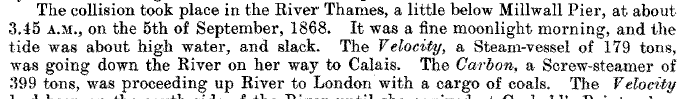
\includegraphics[scale=0.9]{velocity.png}}\attribution{CommonLII}
\end{center}
\caption[`a fine moonlight morning']{`a fine moonlight morning' -- \lawcitesinlinerr(Lord Chelmsford, )(){velocitymnc}[\nopp 268]{velocitynr}[\nopp 727]{velocityer}.
}
\label{fig:velocity}
\end{figure}

\newpage

\noindent \textit{Kerr v Baranow}, 2011 SCC 10, [2011] 1 SCR 269

\noindent \textit{Kerr v Baranow}, 2011 SCC 10 at paras 12-29, 36-39, [2011] 1 SCR 269

\lcsetstylemcgill
\noindent \lawcitesinlinerr[at paras 12-29, 36-39]{kerrmnc}{kerrscr}
\lcsetstyledefault

\noindent \textit{Frame v Smith}, [1987] 2 SCR 99, 42 DLR (4th) 81

\setmulticitecommaon
\setcasenamecommaon
\noindent \lawcitesinlinerr{framescr, framedlr}
\setmulticitecommaoff
\setcasenamecommaoff

%Frame v Smith, [1987] 2 SCR 99, 42 DLR (4th) 81, Dickson CJC.
%
\noindent \textit{McLean v Pilon} (1978), 7 BCLR 99, 1978 CanLII 237 (SC).

\lcsetstylemcgill
\noindent \lawcitesinlinerr{mcleanbclr, mcleanlii}



%==================================================================
\section{Utility Macros}
\lcsetdemooff
\lcsetindexingoff

\optsett{\cmd{lccitedemo}\{key(s)\}}{}\\
\optsett{\cmd{lccitedemorr}\{key(s)\}}{}\\
\optsett{\cmd{lccitedemostat}\{key\}}{}\\
\optsett{\cmd{lccitedemolj}\{key\}}{}\\

These macros display what the citation commands available for an entry type produce. 

\subsection*{Cases}

\lccitedemo{snail}
\bigskip 

\lccitedemo{becker}
\bigskip 

 
\lccitedemorr{armstronglewin, armstronger}
\bigskip 

\lccitedemorr{columbussr, columbusne}\par
\noindent *{\small \textsc{Note}: If the child keys are cited separately, there will be separate entries in the Table of Cases.}
\bigskip 


%=============================================
\subsubsection*{Multicite keys}
%\renewcommand\lcdemolabelw{4cm}
{\small These multicite display tables are hard-coded.}

\noindent\makebox[\lcdemolabelw][l]{\sdfs{lawcitesinline}}\lawcitesinline[\nopp 564]{snail}[\nopp 15]{becker}

\noindent\makebox[\lcdemolabelw][l]{\sdfs{lawcitesinlinerr}}\lawcitesinlinerr[\nopp 200]{columbussr}[\nopp 838]{columbusne}

\noindent\makebox[\lcdemolabelw][l]{\sdfs{lawcitesfoot}}Text\lawcitesfoot[\nopp 564]{snail}[\nopp 15]{becker}

\noindent\makebox[\lcdemolabelw][l]{\sdfs{lawcitesfootrr}}Text\lawcitesfootrr[\nopp 200]{columbussr}[\nopp 838]{columbusne}


%===============================================
\subsection*{Statutes}

\lccitedemostat{crimcan}
\bigskip 

\lccitedemostat{crimnsw}
\bigskip 

\lccitedemostat{canleg}
\noindent *{\small \textsc{Note}: A \texttt{citeref} has priority over any style settings.\footnote{Only Canadian *leg and *reg \texttt{citeref}s have been defined, so far.}}
\bigskip 


\subsection*{Regulations}

\lccitedemostat{canregbc}
\bigskip 


\subsection*{Law Journals}

\lccitedemolj{smythsc}
\bigskip 



%-------------------------------------
\bigskip
\hfill\rulesep\hfill\ %\hrule
\bigskip
%
\printbibliography[
	nottype=case,
	nottype=statute,
	notkeyword=lj,
		]
\printindex


%
\bigskip 

\hfill ----oooOooo---- \hfill\ 
\end{document}